% Options for packages loaded elsewhere
\PassOptionsToPackage{unicode}{hyperref}
\PassOptionsToPackage{hyphens}{url}
\PassOptionsToPackage{dvipsnames,svgnames,x11names}{xcolor}
%
\documentclass[
  12pt,
]{book}
\usepackage{amsmath,amssymb}
\usepackage{lmodern}
\usepackage{setspace}
\usepackage{iftex}
\ifPDFTeX
  \usepackage[T1]{fontenc}
  \usepackage[utf8]{inputenc}
  \usepackage{textcomp} % provide euro and other symbols
\else % if luatex or xetex
  \usepackage{unicode-math}
  \defaultfontfeatures{Scale=MatchLowercase}
  \defaultfontfeatures[\rmfamily]{Ligatures=TeX,Scale=1}
\fi
% Use upquote if available, for straight quotes in verbatim environments
\IfFileExists{upquote.sty}{\usepackage{upquote}}{}
\IfFileExists{microtype.sty}{% use microtype if available
  \usepackage[]{microtype}
  \UseMicrotypeSet[protrusion]{basicmath} % disable protrusion for tt fonts
}{}
\makeatletter
\@ifundefined{KOMAClassName}{% if non-KOMA class
  \IfFileExists{parskip.sty}{%
    \usepackage{parskip}
  }{% else
    \setlength{\parindent}{0pt}
    \setlength{\parskip}{6pt plus 2pt minus 1pt}}
}{% if KOMA class
  \KOMAoptions{parskip=half}}
\makeatother
\usepackage{xcolor}
\IfFileExists{xurl.sty}{\usepackage{xurl}}{} % add URL line breaks if available
\IfFileExists{bookmark.sty}{\usepackage{bookmark}}{\usepackage{hyperref}}
\hypersetup{
  pdftitle={Cambios en la Cohesión Social en Chile},
  pdfauthor={Equipo CEPAL-ELSOC},
  colorlinks=true,
  linkcolor={blue},
  filecolor={Maroon},
  citecolor={Blue},
  urlcolor={Blue},
  pdfcreator={LaTeX via pandoc}}
\urlstyle{same} % disable monospaced font for URLs
\usepackage[left=4cm, right=3cm, top=2.5cm, bottom=2.5cm]{geometry}
\usepackage{longtable,booktabs,array}
\usepackage{calc} % for calculating minipage widths
% Correct order of tables after \paragraph or \subparagraph
\usepackage{etoolbox}
\makeatletter
\patchcmd\longtable{\par}{\if@noskipsec\mbox{}\fi\par}{}{}
\makeatother
% Allow footnotes in longtable head/foot
\IfFileExists{footnotehyper.sty}{\usepackage{footnotehyper}}{\usepackage{footnote}}
\makesavenoteenv{longtable}
\usepackage{graphicx}
\makeatletter
\def\maxwidth{\ifdim\Gin@nat@width>\linewidth\linewidth\else\Gin@nat@width\fi}
\def\maxheight{\ifdim\Gin@nat@height>\textheight\textheight\else\Gin@nat@height\fi}
\makeatother
% Scale images if necessary, so that they will not overflow the page
% margins by default, and it is still possible to overwrite the defaults
% using explicit options in \includegraphics[width, height, ...]{}
\setkeys{Gin}{width=\maxwidth,height=\maxheight,keepaspectratio}
% Set default figure placement to htbp
\makeatletter
\def\fps@figure{htbp}
\makeatother
\setlength{\emergencystretch}{3em} % prevent overfull lines
\providecommand{\tightlist}{%
  \setlength{\itemsep}{0pt}\setlength{\parskip}{0pt}}
\setcounter{secnumdepth}{5}
\newlength{\cslhangindent}
\setlength{\cslhangindent}{1.5em}
\newlength{\csllabelwidth}
\setlength{\csllabelwidth}{3em}
\newlength{\cslentryspacingunit} % times entry-spacing
\setlength{\cslentryspacingunit}{\parskip}
\newenvironment{CSLReferences}[2] % #1 hanging-ident, #2 entry spacing
 {% don't indent paragraphs
  \setlength{\parindent}{0pt}
  % turn on hanging indent if param 1 is 1
  \ifodd #1
  \let\oldpar\par
  \def\par{\hangindent=\cslhangindent\oldpar}
  \fi
  % set entry spacing
  \setlength{\parskip}{#2\cslentryspacingunit}
 }%
 {}
\usepackage{calc}
\newcommand{\CSLBlock}[1]{#1\hfill\break}
\newcommand{\CSLLeftMargin}[1]{\parbox[t]{\csllabelwidth}{#1}}
\newcommand{\CSLRightInline}[1]{\parbox[t]{\linewidth - \csllabelwidth}{#1}\break}
\newcommand{\CSLIndent}[1]{\hspace{\cslhangindent}#1}
\usepackage[utf8]{inputenc}
\usepackage[spanish,es-tabla]{babel}
\usepackage[fixlanguage]{babelbib}
\usepackage{geometry}
\geometry{letterpaper,left=2cm,top=2cm, right=2cm}
\usepackage{times}           
\usepackage{caption}
\captionsetup[figure, table]{labelfont={bf},labelformat={default},labelsep=period}
\usepackage{graphicx}
\usepackage{float}
\usepackage{booktabs}
\usepackage{longtable}
\usepackage{array}
\usepackage{multirow}
\usepackage{wrapfig}
\usepackage{float}
\usepackage{colortbl}
\usepackage{xcolor}
\usepackage{pdflscape}
\usepackage{tabu}
\usepackage{threeparttable}
\usepackage{pdfpages} %para pdf portada

% fuente: https://stackoverflow.com/questions/45963505/coverpage-and-copyright-notice-before-title-in-r-bookdown
%\let\oldmaketitle\maketitle 
%\AtBeginDocument{\let\maketitle\relax}

% \renewcommand{\tablename}{Tabla}
% \ifxetex
%   \usepackage{polyglossia}
%   \setmainlanguage{spanish}
%   % Tabla en lugar de cuadro
%   \gappto\captionsspanish{\renewcommand{\tablename}{Tabla}
%           \renewcommand{\listtablename}{Índice de tablas}}
% \else
%   % \usepackage[spanish,es-tabla]{babel}
% \fi

\usepackage{booktabs}
\usepackage{longtable}
\usepackage{array}
\usepackage{multirow}
\usepackage{wrapfig}
\usepackage{float}
\usepackage{colortbl}
\usepackage{pdflscape}
\usepackage{tabu}
\usepackage{threeparttable}
\usepackage{threeparttablex}
\usepackage[normalem]{ulem}
\usepackage{makecell}
\usepackage{xcolor}
\ifLuaTeX
  \usepackage{selnolig}  % disable illegal ligatures
\fi

\title{Cambios en la Cohesión Social en Chile}
\author{Equipo CEPAL-ELSOC}
\date{2021-10-15}

\begin{document}
\maketitle

{
\hypersetup{linkcolor=}
\setcounter{tocdepth}{1}
\tableofcontents
}
\listoffigures
\listoftables
\setstretch{1.5}
\hypertarget{presentaciuxf3n}{%
\chapter*{Presentación}\label{presentaciuxf3n}}
\addcontentsline{toc}{chapter}{Presentación}

Este reporte de investigación consiste en un análisis de medición y cambios en la cohesión social en Chile en base a indicadores de la Encuesta Longitudinal Social de Chile - \href{https://coes.cl/encuesta-panel/}{ELSOC}, producida por \href{https://coes.cl/}{COES}

Autores:

\begin{itemize}
\tightlist
\item
  Juan Carlos Castillo
\item
  Emmanuelle Barozet
\item
  Vicente Espinoza
\end{itemize}

Ayudante de investigación: Kevin Carrasco.

\hypertarget{introducciuxf3n}{%
\chapter*{Introducción}\label{introducciuxf3n}}
\addcontentsline{toc}{chapter}{Introducción}

El interés por el estudio de la cohesión social posee una larga trayectoria tanto académica como así también desde el estado y de organizaciones con interés público. La cohesión social aparece como una aspiración normativa de una sociedad mejor, vinculada a conceptos como lazos sociales de calidad, pertenencia, y confianza en los demás y en el estado. Se asume también que un estado de adecuada cohesión social es producto de condiciones estructurales y políticas que apunten a mayor igualdad, integración y oportunidades, por lo cual muchas veces se refiere a ella como un horizonte o una consecuencia de buenas políticas sociales. Este interés se ha plasmado en una serie de proyectos internacionales y nacionales que estudian la cohesión social. Por el lado internacional son reconocidas iniciativas como Mapping social Cohesion en Canadá (\protect\hyperlink{ref-jenson_mapping_1998}{Jenson, 1998}) el Scanlon-Monash Cohesion Index en Autralia (\protect\hyperlink{ref-markus_mapping_2014}{Markus, 2014}), el Radar de Cohesión Social en Alemania (\protect\hyperlink{ref-dragolov_social_2013}{Dragolov et al., 2013}), y el proyecto Ecosocial en América Latina Valenzuela et al. (\protect\hyperlink{ref-valenzuela_vinculos_2008}{2008}). En el caso de organizaciones internacionales con foco en América Latina destaca la amplia tradición de la CEPAL en estudios de cohesión social (\protect\hyperlink{ref-cepal_america_2010}{CEPAL, 2010a}, \protect\hyperlink{ref-cepal_cohesion_2010}{2010b}; \protect\hyperlink{ref-cepal_cohesion_2021}{CEPAL, 2021}; \protect\hyperlink{ref-maldonado_inclusion_2020}{Maldonado et al., 2020}; \protect\hyperlink{ref-sojo_cohesion_2007}{Sojo et al., 2007}; \protect\hyperlink{ref-villatoros._sistema_2008}{Villatoro S., 2008})

Muchos de los estudios en cohesión social han tenido como foco su definición y también la búsqueda de indicadores para poder caracterizar distintas sociedades respecto a sus niveles de cohesión social en sus múltiples dimensiones. Parte de este objetivo lo comparte el Centro de Estudios de Conflicto y Cohesión Social (COES), al cual pertenecen las/os autores de este trabajo, y que dados los intereses comunes con CEPAL han venido trabajando hace algunos años en distintas iniciativas, tales como el informe sobre Clases Medias y Cohesión Social recientemente publicado por CEPAL (\protect\hyperlink{ref-barozet_clases_2021}{Barozet et al., 2021}). El presente trabajo se enmarca en esta relación de colaboración, y se enfoca en la definición y medición de indicadores de cohesión social basado en el concepto de cohesión social recientemente actualizado por la CEPAL (\protect\hyperlink{ref-cepal_cohesion_2021}{CEPAL, 2021}) que señala que:

\textbf{``la cohesión social puede ser comprendida como la capacidad de una sociedad y sus instituciones democráticas de promover relaciones sociales de igualdad y generar un sentido de pertenencia y una orientación hacia el bien común de una forma percibida como legítima por sus miembros. Esa capacidad requiere de la existencia de garantías de bienestar, la promoción activa de una cultura de la igualdad, de mecanismos para la reducción de las desigualdades, de reconocimiento, de participación y para la resolución pacífica de conflictos y adaptación a cambios, en el marco de un Estado de derecho y una democracia de calidad''}. (\protect\hyperlink{ref-cepal_cohesion_2021}{CEPAL, 2021})

La primera parte de esta definición de cohesión social como capacidad hace referencia a una serie de elementos constitutivos del concepto de cohesión social, y que se pueden encontrar en otras definiciones contemporáneas de cohesión como las del \href{https://www.bertelsmann-stiftung.de/en/publications/publication/did/social-cohesion-radar/}{Radar de la Cohesión Social} y las del \href{https://www.desarrollosocialyfamilia.gob.cl/storage/docs/Informe_Final_Consejo_Cohesion_Social.pdf}{Consejo Asesor para la Cohesión Social} desarrollada en Chile el año 2020, y que entienden la cohesión como un fenómeno multidimensional. Gran parte de la literatura y estudios empíricos a la fecha en el área se han enfocado en generar mediciones e indicadores para cada una de estas subdimensiones, para lo cual utilizan datos secundarios de encuestas nacionales e internacionales y así realizar un diagnóstico del estado de la cohesión social.

En Chile es posible identificar dos estudios específicos que se han abocado a la medición de los elementos constitutivos de la cohesión social basados en encuestas: Ecosocial (\protect\hyperlink{ref-valenzuela_vinculos_2008}{Valenzuela et al., 2008}) y \href{https://coes.cl/encuesta-panel/}{ELSOC}(Estudio Longitudinal Social de Chile). Ecosocial es una encuesta ``construida con el propósito de medir y documentar una serie de aspectos relacionados con el estado de la cohesión social en la población de las principales ciudades de siete países Latinoamericanos: Argentina, Brasil, Colombia, Chile, Guatemala, México y Perú.'' (\protect\hyperlink{ref-valenzuela_vinculos_2008}{Valenzuela et al., 2008, p. 5}). Los resultados de esta encuesta han sido publicados en libros como \href{https://www.cieplan.org/wp-content/uploads/2019/12/Libro_Completo_Vinculos_Creencia_e_Ilusiones.pdf}{``Vínculos, Creencias e Ilusiones''} (2008), en conexión con otros trabajos también de CIEPLAN centrados en cohesión como el libro \href{https://www.cieplan.org/wp-content/uploads/2019/12/Libro_Completo_Redes_Estado_y_Mercado_compressed.pdf}{``Redes, Estado y Mercado''}(2008). En cuanto a la encuesta \href{https://coes.cl/encuesta-panel/}{ELSOC}, es un panel longitudinal desarrollado por el Centro de Estudios de Conflicto y Cohesión Social \href{https://www.coes.cl/}{COES}, y que será la base de datos principal para el presente estudio dado su carácter longitudinal que permite analizar cambios en la cohesión social en el tiempo.

El principal objetivo de la encuesta ELSOC es evaluar la manera como piensan, sienten y se comportan las y los chilenos en torno a un conjunto de temas referidos al conflicto y la cohesión social en Chile. Además, permite comparar la estabilidad o cambio en diversas dimensiones sociales atendiendo a factores que los moderan o explican a lo largo de los años. Para ello se encuesta anualmente desde el año 2016 a alrededor de 3.000 personas de manera longitudinal mediante panel, es decir, todos los años se encuesta a las mismas personas para así analizar cambios en trayectorias individuales en distintos temas. Los temas abordados en esta encuesta así como su naturaleza longitudinal la hacen única en el país y permite despejar una serie de preguntas sobre cambio social que no pueden ser abordadas con precisión con la comparación de encuestas repetidas en el tiempo a distintos sujetos (mayores detalles de este estudio se presentan al principio del capítulo 1).

El presente documento se estructura en tres capítulos principales. El primer capítulo está abocado a la medición de la cohesión social, donde se proponen indicadores de la encuesta ELSOC para las distintas subdimensiones de cohesión social propuestas por CEPAL. El segundo capítulo toma estos indicadores por dimensión y subdimensión y analiza su cambio/estabilidad en el tiempo en Chile entre 2016 y 2020. Finalmente, el capítulo 3 ahonda en los determinantes sociales de los posibles cambios detectados en el capítulo 2.

\hypertarget{generaciuxf3n-de-indicadores-de-cohesiuxf3n-social}{%
\chapter{Generación de indicadores de cohesión social}\label{generaciuxf3n-de-indicadores-de-cohesiuxf3n-social}}

El objetivo de este primer capítulo es establecer indicadores de cohesión social basados en el modelo conceptual de CEPAL, en particular para los denominados \emph{elementos constitutivos de la cohesión social} y que se presentan en la Figura \ref{fig:esquema-cepal}.

\begin{figure}[H]

{\centering 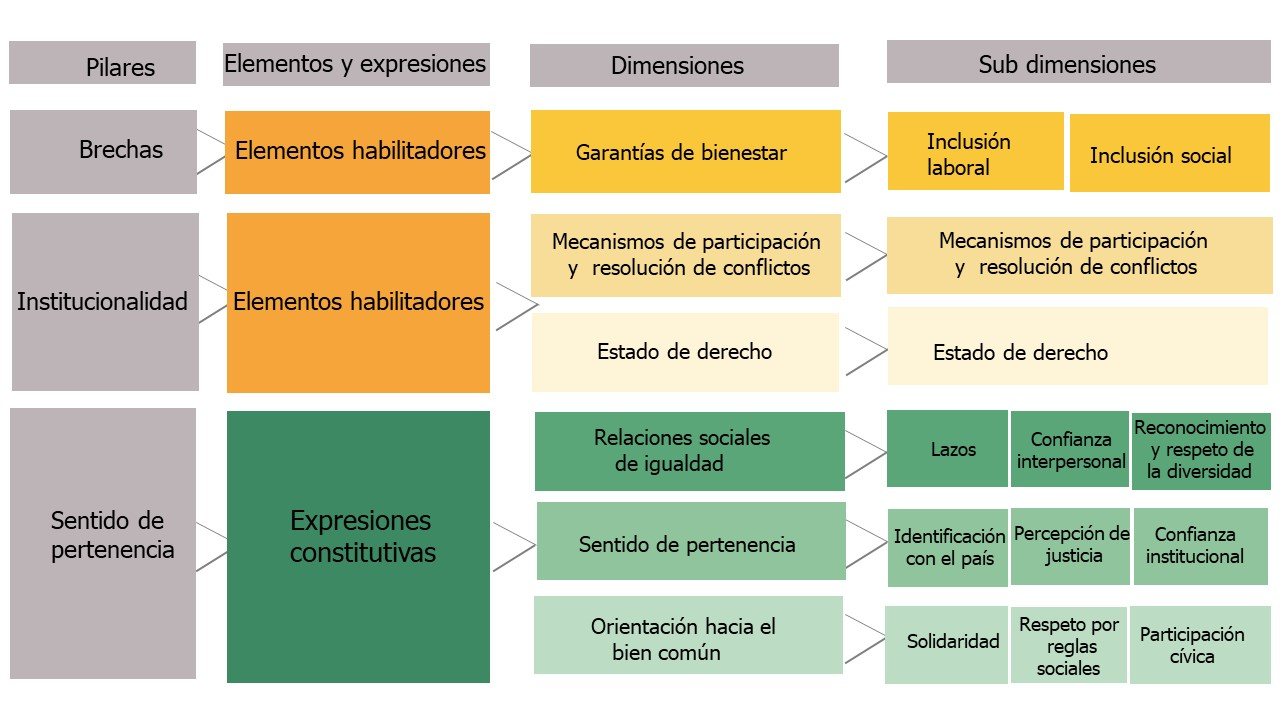
\includegraphics[width=1\linewidth,height=1\textheight]{images/dimensiones-cepal} 

}

\caption{Resumen dimensiones CEPAL.}\label{fig:esquema-cepal}
\end{figure}

El modelo de cohesión social de la CEPAL se caracteriza por ser de naturaleza \textbf{multidimensional}, es decir, podemos decir que la cohesión social no se puede reducir a una única dimensión ni medición, sino que debe ser abordado considerando distintos componentes o dimensiones. La investigación más actual sobre cohesión social asume esta perspectiva y en gran medida coincide con las dimensiones identificadas por CEPAL, como son relaciones sociales de igualdad, sentido de pertenencia y orientación hacia el bien común (\protect\hyperlink{ref-schiefer_essentials_2016}{Schiefer \& Noll, 2016}). Este tipo de modelos multidimensionales también se caracterizan por el establecimiento de subdimensiones e indicadores para cada uno de ellos, que es el objetivo principal de este primer capítulo.

\emph{Datos}

En este capítulo y los siguientes se utilizaran los datos de la encuesta \href{https://coes.cl/encuesta-panel/}{\textbf{ELSOC} (Estudio Longitudinal Social de Chile)} que se asocien al contenido de cada una de las dimensiones y subdimensiones del concepto de cohesión social. La selección de esta encuesta para este estudio se basa no solamente en la presencia de indicadores de cohesión social, sino también en que permitirá analizar cambios anuales de \textbf{trayectorias individuales} en dimensiones y subdimensiones de cohesión social entre 2016 y 2020. Dado que en esta encuesta panel se entrevista a las mismas personas año a año (N=3.000 app.), es posible analizar cambios en el tiempo de manera más precisa que mediante la comparación de distintas muestras en distintos momentos (donde no es posible precisar si los cambios en los indicadores se asocian a un momento distinto o a que las personas son distintas).

La encuesta ELSOC es aplicada por medio de un cuestionario estructurado que posee 7 módulos diferentes: Territorio, Redes y actitudes sociales, Ciudadanía y democracia, Desigualdad y legitimidad, Conflicto social, Salud y bienestar y Caracterización sociodemográfica. Posee un muestreo probabilístico, estratificado (por tamaño de ciudades), por conglomerados y multietápico (aleatorio en todas sus etapas). En el muestreo probabilístico de ELSOC se seleccionaron aleatoriamente 40 ciudades con más de 10.000 habitantes (92 comunas de 13 regiones), dentro de estas se escogieron aleatoriamente 1067 manzanas. Luego, en cada manzana se escogieron hogares aleatoriamente y dentro de cada hogar fueron elegidos también de manera aleatoria personas de 18 años o más. Por lo tanto, su unidad básica de observación son personas. Asimismo, la población objetivo son hombres y mujeres de 18 a 75 años. Esta encuesta alcanza un 77\% de representatividad de la población total del país y un 93\% de la población urbana, con un error muestral del 2\% (\protect\hyperlink{ref-coes_radiografia_2019}{COES, 2019}). La muestra alcanzada en 2020 posee las respuestas de 2741 individuos, que incluye respuestas de participantes de la primera ola (2016) y de la muestra de refresco iniciada en 2018.

\textbf{Sobre medición de dimensiones y subdimensiones de cohesión social con la encuesta ELSOC}

Para la selección de items de la encuesta se privilegian aquellos que se repiten en las distintas versiones (olas) de la encuesta, de manera de permitir la comparación en el tiempo. Existen también algunos items que aparecen de manera intercalada (cada dos años), y que se utilizan en caso de requerir mayor información para medir las subdimensiones de cohesión social. Los análisis en este capítulo se realizan con los items de la primera ola (2016), y en el caso de items intercalados que aparezcan desde el 2017 se utilizan los correspondientes a ese año.

Dado que la encuesta ELSOC no fue diseñada específicamente en base al modelo de cohesión de CEPAL, en este capítulo se identificarán aquellos items que se relacionan más cercanamente a cada uno de los conceptos presentes en las subdimensiones. Para ello también se tomará como referencia la propuesta de items elaborada por la CEPAL basada en encuestas comparativas de América Latina. Luego de esta identificación se procederá a un análisis descriptivo y de asociaciones entre los items que conforman cada subdimension, y en base a ello se realizará una propuesta de medición de subdimensiones en base a indicadores.

Antes de comenzar con el trabajo de análisis de subdimensiones e indicadores, es pertinente hacer algunos alcances sobre lo que se entiende por \emph{medición}. En este contexto, medición hace referencia a otorgar propiedades numéricas a ciertos atributos individuales en base a ciertas reglas. Este proceso por definición no es exacto y conlleva error, ya que muchos de los conceptos que se trabajan en ciencias sociales no se pueden medir directamente y se consideran por lo tanto constructos latentes (como clase, estatus, pertenencia, confianza, entre muchos otros). Gran parte del trabajo de buscar evidencia de validez de las mediciones se trata justamente de cuantificar y minimizar este error. Para esto no solo basta con un análisis de \emph{validez aparente}, referido a que el contenido de los items parezca relacionarse con el concepto que se desea medir, sino también con las propiedades métricas del indicador, como son la variabilidad y covariabilidad/correlación con otras medidas asociadas. Es por ello que en medición muchas veces se utilizan indicadores múltiples para un mismo concepto - sobre todo aquellos de naturaleza compleja y multidimensional como cohesión social -, de modo de identificarlo y estimarlo de una manera más robusta con técnicas específicas de análisis de constructos latentes.

La breve mención a aspectos de medición del párrafo anterior permite aclarar el orden y el sentido del análisis que se presenta a continuación. En algunos casos encontraremos items únicos para las subdimensiones, y en este caso no tenemos mayor alternativa que discutir su validez aparente y esperar un bajo nivel de error de medición. En otros casos existen baterías de items múltiples, donde se propondrán indicadores que representen de mejor manera los elementos comunes (covarianza) y que subyacen a la batería, para lo que se utilizarán técnicas de análisis factorial.

Las decisiones respecto de los indicadores de cohesión social variarán según sea el número de items presentes por subdimensión:

\begin{itemize}
\item
  1 item: se considerará simplemente el puntaje de la variable.
\item
  2 items: se analizará la correlación entre ambas y sobre esta base se podrá proponer un promedio simple.
\item
  3 items: se analizará la matriz de correlaciones y el alfa de Cronbach como medida de consistencia interna que permita trabajar con el promedio de los items. Esta medida, que se aproxima a un promedio de las correlaciones entre los items, otorga un número que va entre 0 y 1, y donde el nivel convencional para considerar consistencia es 0.7 o mayor.
\item
  4 items o más: se realizará un análisis factorial exploratorio para evaluar la dimensionalidad subyacente a los items, y en base a este análisis se propondrá un promedio con los indicadores correspondientes a el/los factor(es) que mejor representen la variabilidad subyacente.
\end{itemize}

A continuación se presenta el análisis ordenado por dimensiones y subdimensiones:

\begin{itemize}
\tightlist
\item
  Dimensión relaciones sociales de igualdad:

  \begin{itemize}
  \tightlist
  \item
    confianza interpersonal
  \item
    reconocimiento y respecto de la diversidad
  \item
    lazos
  \end{itemize}
\item
  Dimensión sentido de pertenencia:

  \begin{itemize}
  \tightlist
  \item
    identificación con el país
  \item
    percepción de justicia
  \item
    confianza institucional
  \end{itemize}
\item
  Dimensión orientación hacia el bien común:

  \begin{itemize}
  \tightlist
  \item
    solidaridad
  \item
    participación cívica
  \end{itemize}
\end{itemize}

Por ejemplo, considerando en primer lugar la dimensión ``Relaciones Sociales de Igualdad'', comenzamos con la subdimensión ``confianza interpersonal'' identificando items de la encuesta que representen este concepto, y con la información disponible elaboramos una propuesta para cubrir cada una de las subdimensiones.

Estas tres dimensiones provienen del modelo presentado por la CEPAL, que centra su atención en el nivel nacional y que utiliza fuentes de datos que permiten una comparabilidad entre países. Ya que en este caso estamos utilizando una encuesta nacional, no deja de ser relevante abordar una dimensión territorial que permita complementar y enriquecer el análisis a nivel de país. Por lo tanto, además de las dimensiones del modelo de la CEPAL, de manera exploratoria se agrega una cuarta dimensión de cohesión social en el territorio, que se asocia a la confianza en vecinos, identificación barrial, sociabilidad barrial y satisfacción residencial.

\textbf{Resumen de la propuesta de medición de la cohesión social}

La propuesta de medición de la cohesión social generada en este informe a partir de los criterios propuestos y de los análisis realizados incluye el siguiente conjunto de indicadores para cada una de las dimensiones, que se muestra en la Tabla \ref{tab:descriptivos-cohesion}.

\label{tab:descriptivos-cohesion}Descriptivos medición de cohesión social.

Subdimensión

Indicadores

Min - max

Mean (sd)

Lazos

Cantidad de personas que se conocen con diferentes ocupaciones (2016)

1 - 5

3.941 (0.949)

Confianza interpersonal

Se puede confiar en la mayoria de las personas (2016).

1 - 3

1.314 (0.529)

La mayoria de las personas tratan de ayudar a las demas (2016).

Reconocimiento y respeto de la diversidad

Grado de confianza con personas homosexuales (2016).

1 - 5

2.752 (1.059)

Grado de confianza con personas mapuche (2016).

Grado de confianza con personas inmigrantes (2016).

Identificación con el país

Me siento orgulloso de ser chileno (2016).

4.245 (0.671)

Me identifico con Chile (2016).

Percepción de justicia

En Chile las personas son recompensadas por sus esfuerzos (2016).

2.67 (0.977)

En Chile las personas son recompensadas por su inteligencia (2016).

Confianza institucional

Confianza en el gobierno (2016).

1.799 (0.786)

Confianza en el presidente/a de la republica (2016).

Confianza en los partidos politicos (2016).

Solidaridad

Ha donado dinero a una obra social o de caridad (2016).

1 - 3

2.169 (0.591)

Ha prestado una suma de dinero de \$10.000.- o mas (2016).

Ha conversado con una persona en problemas o deprimida (2016).

Ha ayudado a alguien a conseguir trabajo (2016).

Participación cívica

Firmado una carta o peticion apoyando una causa (2016).

1 - 4.75

1.475 (0.657)

Asistido a una marcha o manifestacion pacifica (2016).

Participado en una huelga (2016).

Usado las redes sociales para expresar su opinion en temas publicos (2016).

Cohesión territorial

Este barrio es ideal para mi (2016).

1 - 5

3.625 (0.839)

Me siento integrado/a en este barrio (2016).

Me identifico con la gente de este barrio (2016).

Este barrio es parte de mi (2016).

A continuación se detallan los criterios y análisis utilizados para seleccionar el conjunto de indicadores que constituyen la propuesta de medición de la cohesión social.

\hypertarget{relaciones-sociales-de-igualdad}{%
\section{Relaciones sociales de igualdad}\label{relaciones-sociales-de-igualdad}}

De acuerdo a la CEPAL, ``esta parte de la definición de la cohesión social se acerca a aquellas que conciben la cohesión social como el compromiso y habilidad para trabajar juntos, incluso cuando los valores que poseen las personas sean distintos (Comisión Económica para África, 2016; Pornschlegel y Jürgensen, 2019; Dragolov y otros, 2013; De Beer, 2014; Woolcock, 2011; Banco Mundial, 2012, 2000; Stanley, 2003). Supone asimismo el principio de reconocimiento recíproco como precondición de la cohesión social (véase, por ejemplo, Jenson, 1998), así como la superación de todas las formas de discriminación'' (\protect\hyperlink{ref-cepal_cohesion_2021}{CEPAL, 2021, p. 45}). Las subdimensiones que componen esta dimensión son confianza interpersonal, reconocimiento de la diversidad, y lazos.

\textbf{Confianza interpersonal}

La confianza interpersonal es un atributo de las relaciones sociales que permite la interacción intergrupal y facilita la acción colectiva a favor de los objetivos compartidos. Por lo tanto, ``la confianza se considera un habilitador de la cooperación y participación (capital social)'' (\protect\hyperlink{ref-cepal_cohesion_2021}{CEPAL, 2021, p. 74}).

En la propuesta regional de CEPAL se utilizan los indicadores ``Confianza en la gente de su comunidad'', que busca cuantificar que tan confiable consideran a los habitantes de su comunidad y ``Confianza en la gente que se conoce por primera vez'', en el cual se cuantifica si se puede confiar en la mayoría de las personas o uno debe ser cuidadoso con los demás. Al trabajar con ELSOC, los items que van en esta línea son ``Se puede confiar en la mayoría de las personas o hay que tener cuidado al tratar con ellas'', ``La mayoría de las personas tratan de ayudar a las demás o se preocupan sólo de sí mismas'' y ``La mayoría de la gente intentaría aprovecharse de usted o la gente trata de ser justa'', presentes en las cinco versiones de ELSOC. Un análisis descriptivo de estos items se presenta en la Figura \ref{fig:confianza-interpersonal} y un análisis bivariado en la Figura \ref{fig:confianza-interpersonal-cor}.

\begin{figure}[H]

{\centering 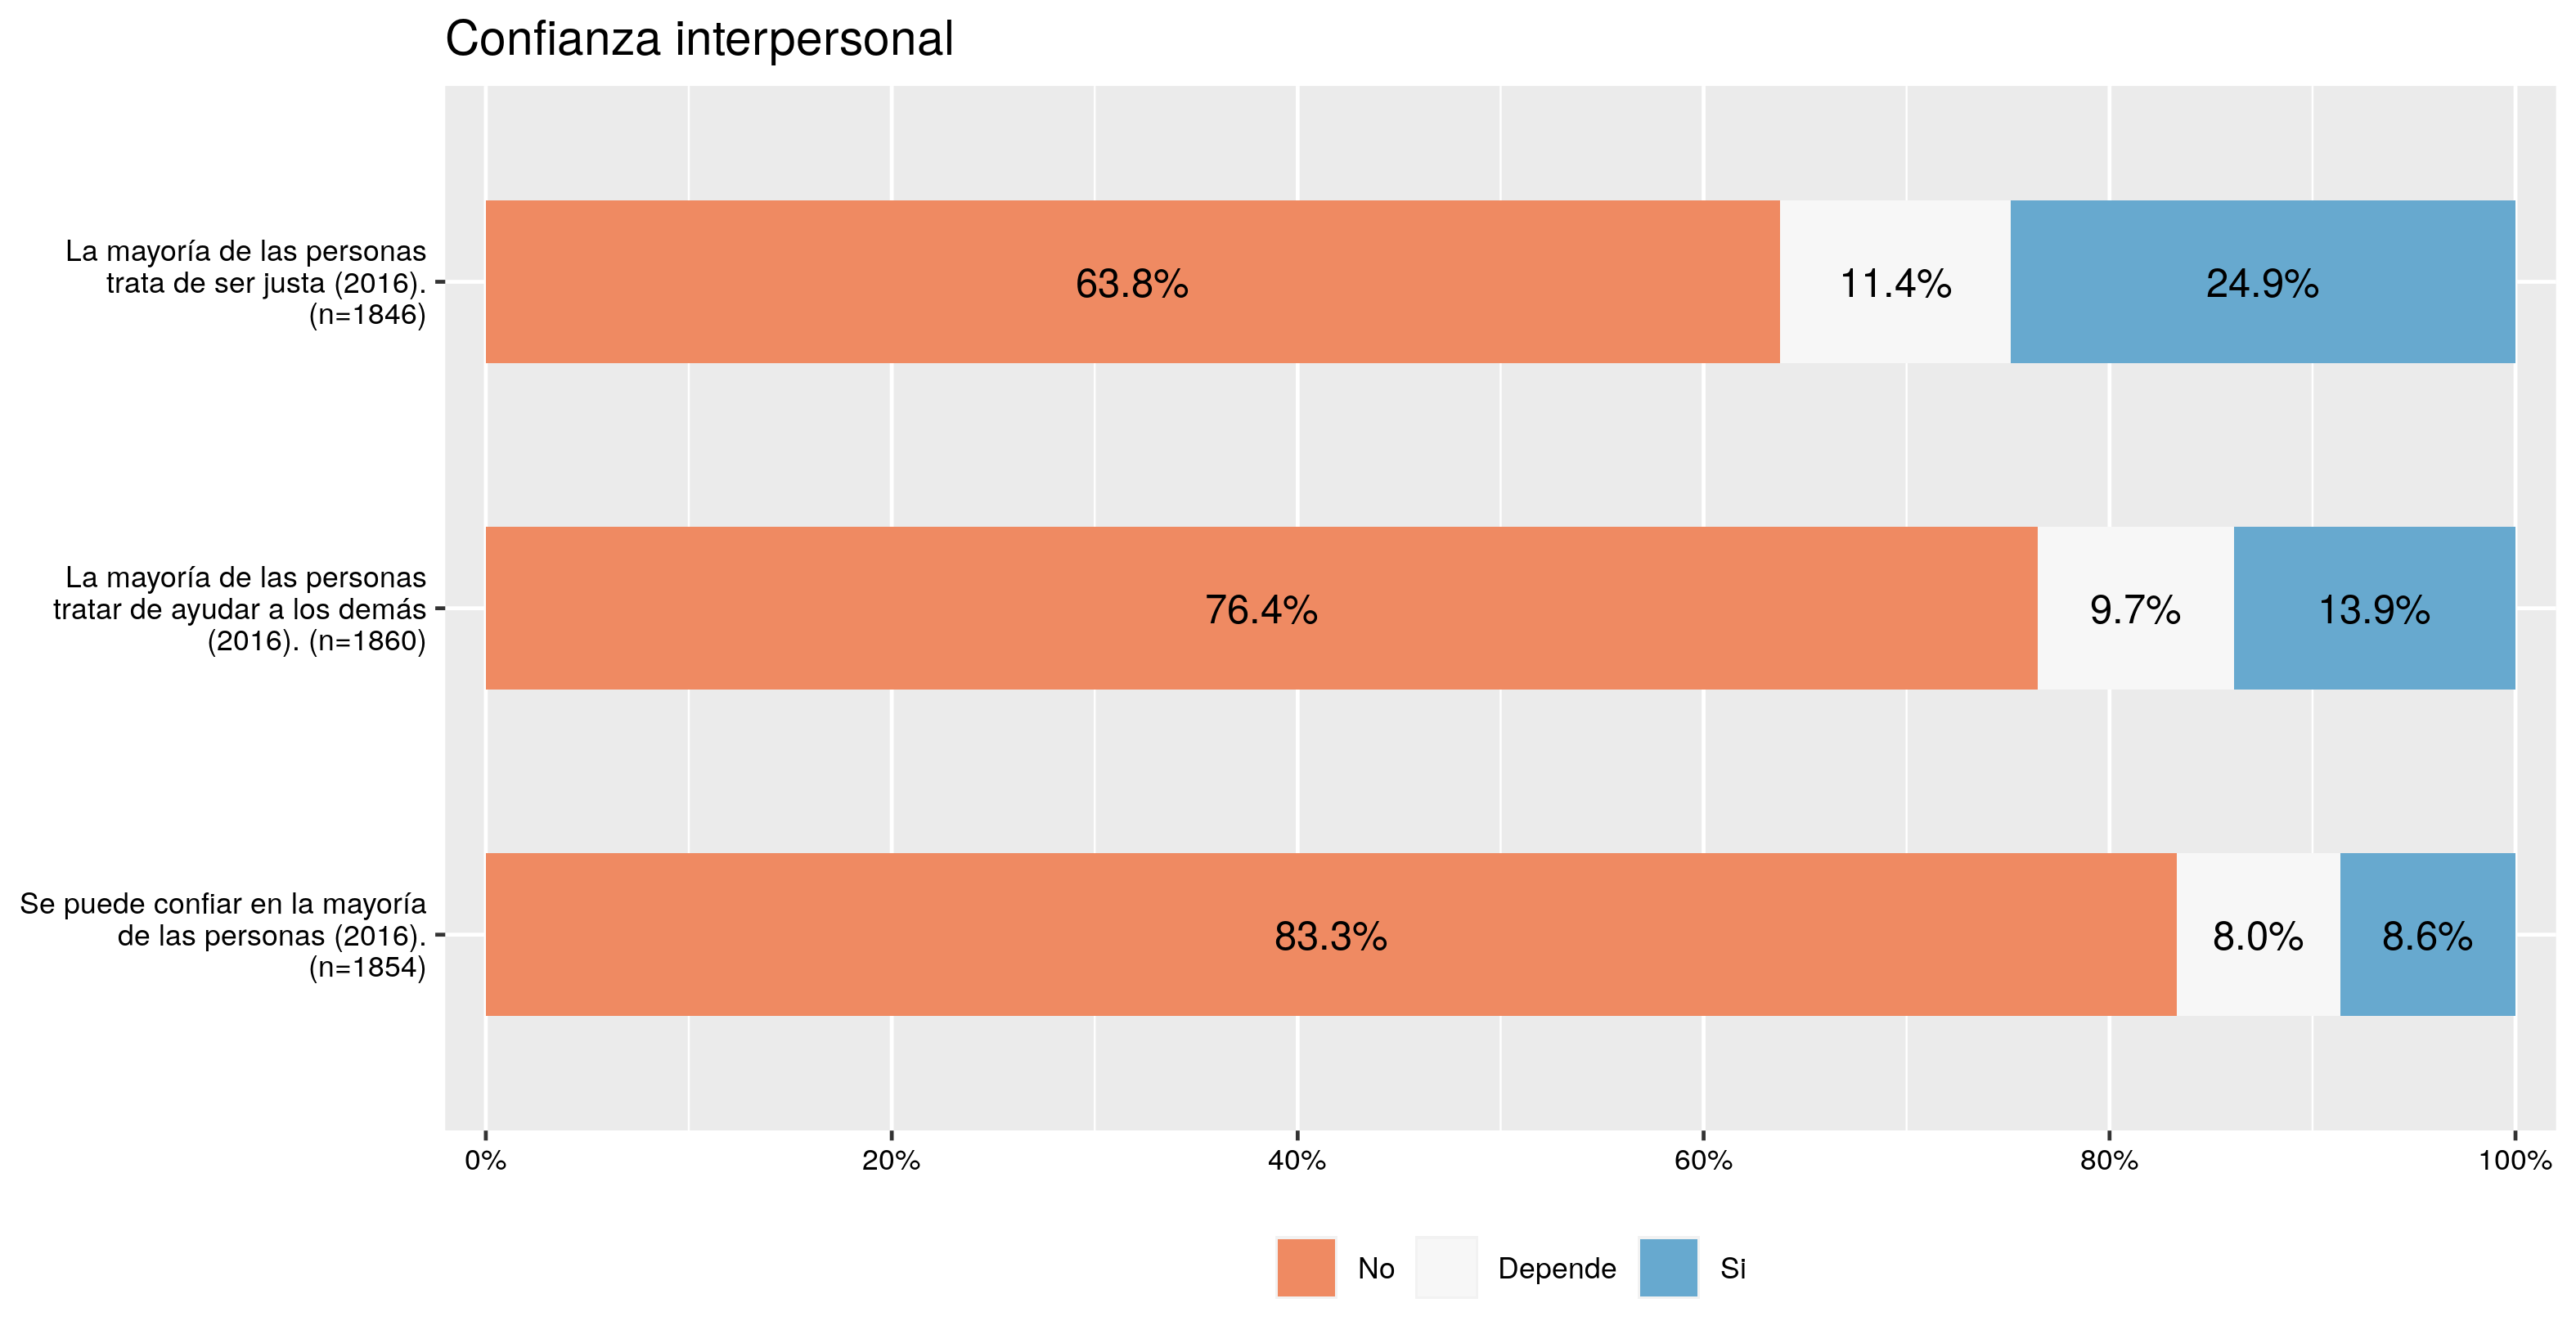
\includegraphics[width=1\linewidth,height=1\textheight]{output/graphs/confianza-interpersonal} 

}

\caption{Confianza interpersonal.}\label{fig:confianza-interpersonal}
\end{figure}

En la matriz de correlaciones de la Figura \ref{fig:confianza-interpersonal-cor} vemos que las correlaciones entre los items van en el rango bajo a moderado, donde los items más correlacionados son A y B. Al calcular la consistencia interna de estos tres items mediante alpha de Cronbach el resultado arroja 0.42, bastante por debajo del límite recomendable de 0.7. Por lo tanto, el índice sugerido para esta subdimensión considera un promedio solo de aquellos items que presentan una correlación mayor: ``Se puede confiar en la mayoría de las personas'' y ``La mayoría de las personas trata de ayudar a los demás''.

\begin{figure}[H]

{\centering 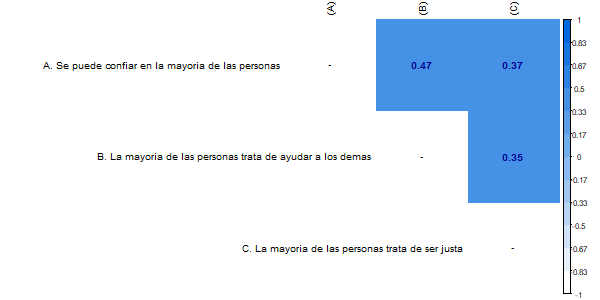
\includegraphics[width=1\linewidth,height=1\textheight]{output/graphs/confianza-interpersonal_cor} 

}

\caption{Asociación indicadores Confianza interpersonal.}\label{fig:confianza-interpersonal-cor}
\end{figure}

\textbf{Reconocimiento y respeto de la diversidad}

Las relaciones sociales de igualdad suponen el reconocimiento de la dignidad del ``otro'' y el reconocimiento de ser parte de una comunidad de iguales en materia de derechos ciudadanos, siendo un elemento que surge de la interacción en redes y asociaciones con individuos de distintas características (\protect\hyperlink{ref-cepal_cohesion_2021}{CEPAL, 2021}).

En la propuesta regional de CEPAL se utilizan dos indicadores en esta subdimensión: ``Aprueba el derecho a contraer matrimonio de parejas del mismo sexo'', que se incluye con el objetivo de cuantificar la tolerancia hacia los individuos y comunidades con distinta orientación sexual y ``Los hombres no tienen prioridad sobre la mujer, a la hora acceder a un trabajo'', que se incluye con el objetivo de cuantificar la cultura de igualdad de género en la sociedad. Además, en la propuesta regional de la CEPAL se deja pendiente la construcción de un indicador sobre tolerancia a personas de distinta raza y etnia, así como de percepción de discriminación debido a la ausencia de indicadores comparables a nivel regional. En el caso de ELSOC existen items distintos pero relacionados con actitudes hacia la diversidad: a) Chile pierde su identidad con la llegada de inmigrantes; b) Con la llegada de inmigrantes aumenta el desempleo; c) Grado de acuerdo con adopción homoparental; d) Grado de confianza con personas homosexuales; e) Grado de confianza con personas mapuche; y f) Grado de confianza con personas inmigrantes. Los dos primeros items están presentes en las cinco versiones, adopción homoparental en olas 2018 y 2019 y el resto de items en las olas 2017 y 2019. Un gráfico descriptivo de estos items se presenta en la Figura \ref{fig:prejuicios} y en la Figura \ref{fig:diversidad} y un análisis bivariado en la Figura \ref{fig:diversidad-cor}.

\begin{figure}[H]

{\centering 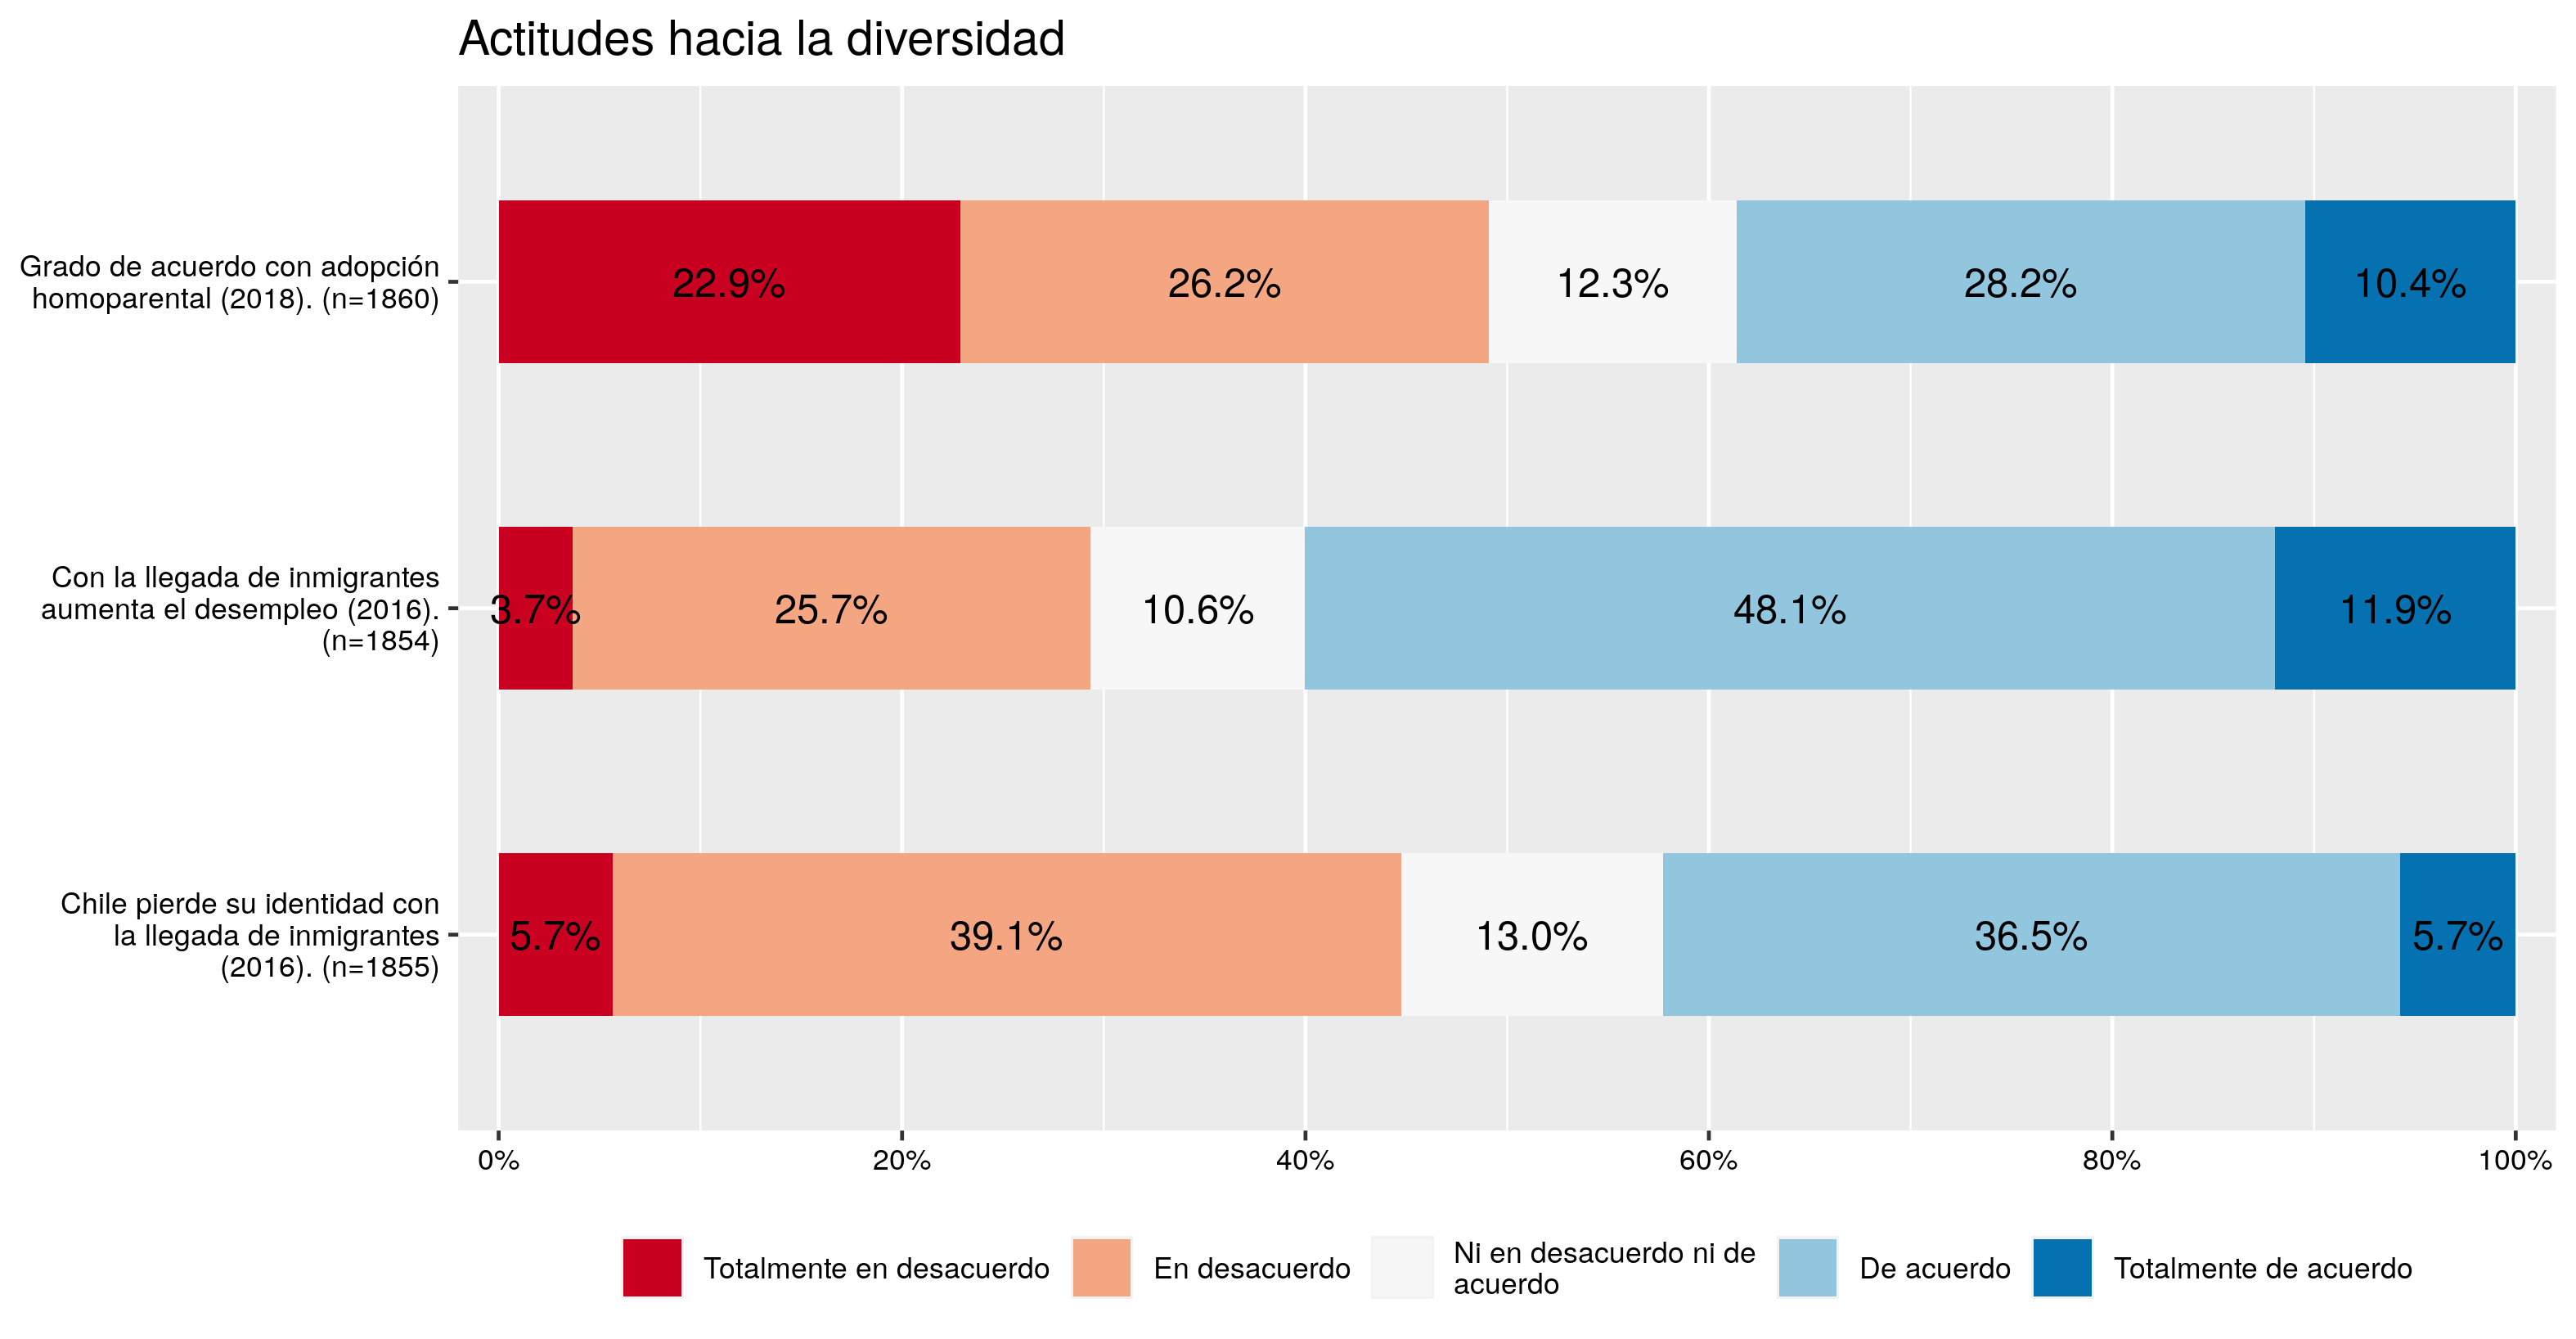
\includegraphics[width=1\linewidth,height=1\textheight]{output/graphs/prejuicios} 

}

\caption{Prejuicios hacia inmigrantes y adopción homoparental.}\label{fig:prejuicios}
\end{figure}

\begin{figure}[H]

{\centering 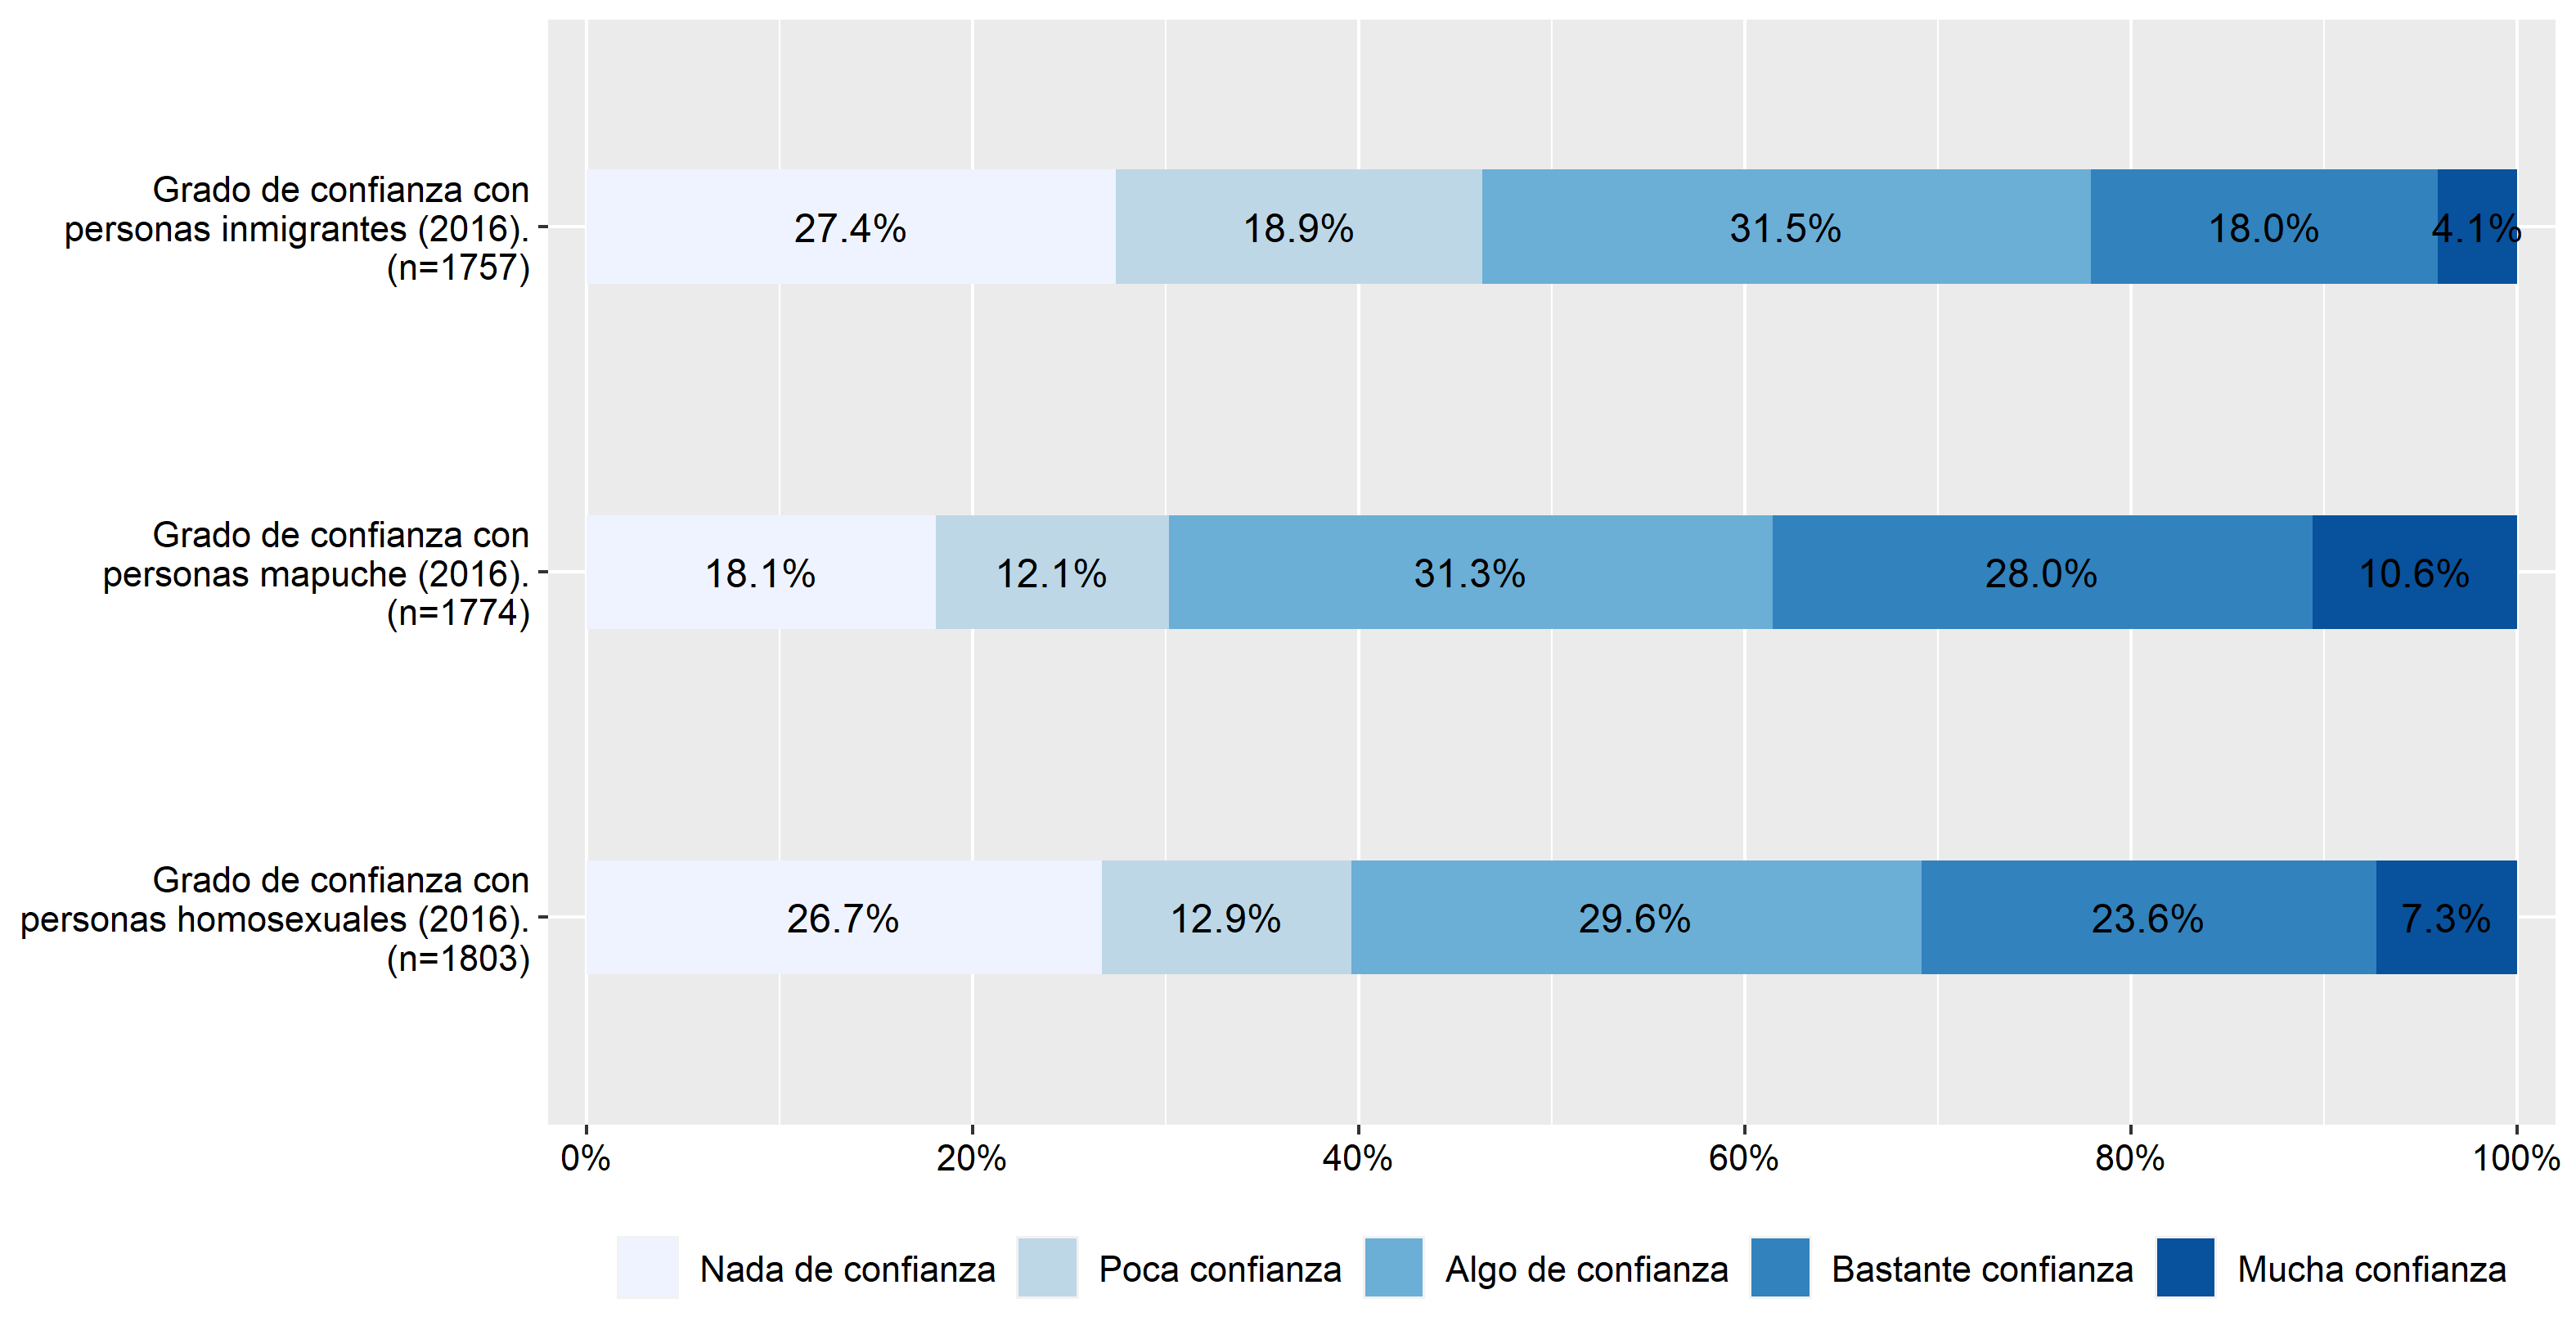
\includegraphics[width=1\linewidth,height=1\textheight]{output/graphs/diversidad} 

}

\caption{Grado de confianza grupos sociales.}\label{fig:diversidad}
\end{figure}

\begin{figure}[H]

{\centering 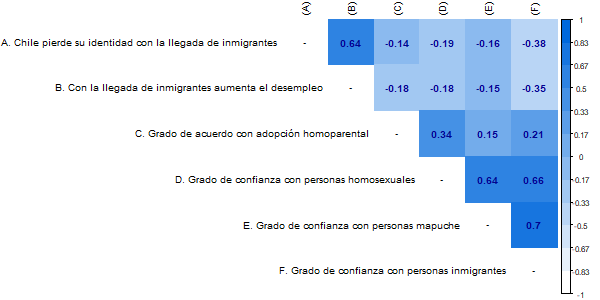
\includegraphics[width=1\linewidth,height=1\textheight]{output/graphs/diversidad_cor} 

}

\caption{Asociación de indicadores de la subdimensión Reconocimiento y respeto de la diversidad.}\label{fig:diversidad-cor}
\end{figure}

Dada la cantidad de items y la heterogeneidad de sus correlaciones, es necesario realizar análisis adicionales. Para ello utilizaremos análisis factorial exploratorio, que entrega información de las dimensiones comunes que subyacen a un conjunto de items. La Tabla \ref{tab:div-fa} muestra el resultado de la extracción de tres factores:

\begin{longtable}[]{@{}l@{}}
\caption{\label{tab:div-fa}Dimensiones de reconocimiento y respeto de la diversidad.}\tabularnewline
\toprule
\endhead

\includegraphics[width=8.33333in,height=\textheight]{output/tables/div_fa.png} \\
\bottomrule
\end{longtable}

En la Tabla \ref{tab:div-fa} observamos en la primera columna los items analizados, y las siguientes columnas que comienzan con ML se refieren a cada uno de los factores extraídos, en este caso tres. Los valores de la tabla en estas columnas indican la intensidad de la relación entre items y factores en una escala de 0 a 1, donde sobre 0.7 se asume una asociación considerable entre item y factor. La columna \emph{Uniqueness} (unicidad) se refiere a la proporción de varianza que el indicador no comparte con los factores (varianza única), y la fila \emph{Proportion Var} al final de la tabla informa la proporción de la varianza del factor en relación a la varianza total.

En la segunda columna (ML1) se observa un factor que se relaciona con las preguntas sobre el grado de confianza de la Figura \ref{fig:diversidad}, luego un segundo factor asociado a las preguntas de inmigrantes, y finalmente un tercer factor asociado a la pregunta de adopción homoparental. Atendiendo ahora a la varianza asociada a estos factores, el primer factor representa casi un 30\% de la varianza, el segundo alrededor de 20\% y el tercero muy por debajo con cerca de un 11\%. Por lo tanto existe mayor consistencia en los dos primeros factores, y entre ellos dos el asociado a confianza hacia la diversidad es el más nítido. Basándose en este análisis es posible proponer utilizar un índice que represente a la subdimensión de reconocimiento y respeto hacia la diversidad calculado a partir de un promedio simple entre los indicadores ``Grado de confianza con personas mapuche'', ``Grado de confianza con personas inmigrantes'' y ``Grado de confianza con personas homosexuales''.

\textbf{Lazos}

Según la CEPAL (\protect\hyperlink{ref-cepal_cohesion_2021}{2021}), ``los lazos sociales permiten generar espacios de cooperación que faciliten el desarrollo de relaciones sociales de igualdad, y establece patrones de reciprocidad interpersonal (PNUD, 2013)'' (p.~74)

El indicador utilizado en la propuesta regional de la CEPAL para esta subdimensión es ``Importancia de los amigos en la vida'', que es un indicador de percepción de la Encuesta Mundial de Valores, a partir del cual se busca cuantificar la intensidad del tejido social en los países de la región. En el caso de ELSOC los items más cercanos a esta operacionalización corresponden a ``Cantidad de amigos/as cercanos'' y ``Tamaño de la red cercana'', que están presentes solo en las olas de los años 2017 y 2019 de la encuesta. Además, se incluye un item de ``Cantidad de personas que se conocen con diferentes ocupaciones'' (gerentes de empresas, vendedor ambulante, secretario/a, mecánico de autos, vendedor de tienda, abogado/a, aseador/a de oficina, médico, parvularia, chofer de taxi, camarero/a, contador/a, profesor/a universitario) para determinar la heterogeneidad de los lazos; este item está presente en las versiones 2016, 2018 y 2020.

La Figura \ref{fig:lazos} muestra un gráfico descriptivo de estos items, mientras en la Figura \ref{fig:lazos-cor} se presenta la estimación de las correlaciones.

\begin{figure}[H]

{\centering 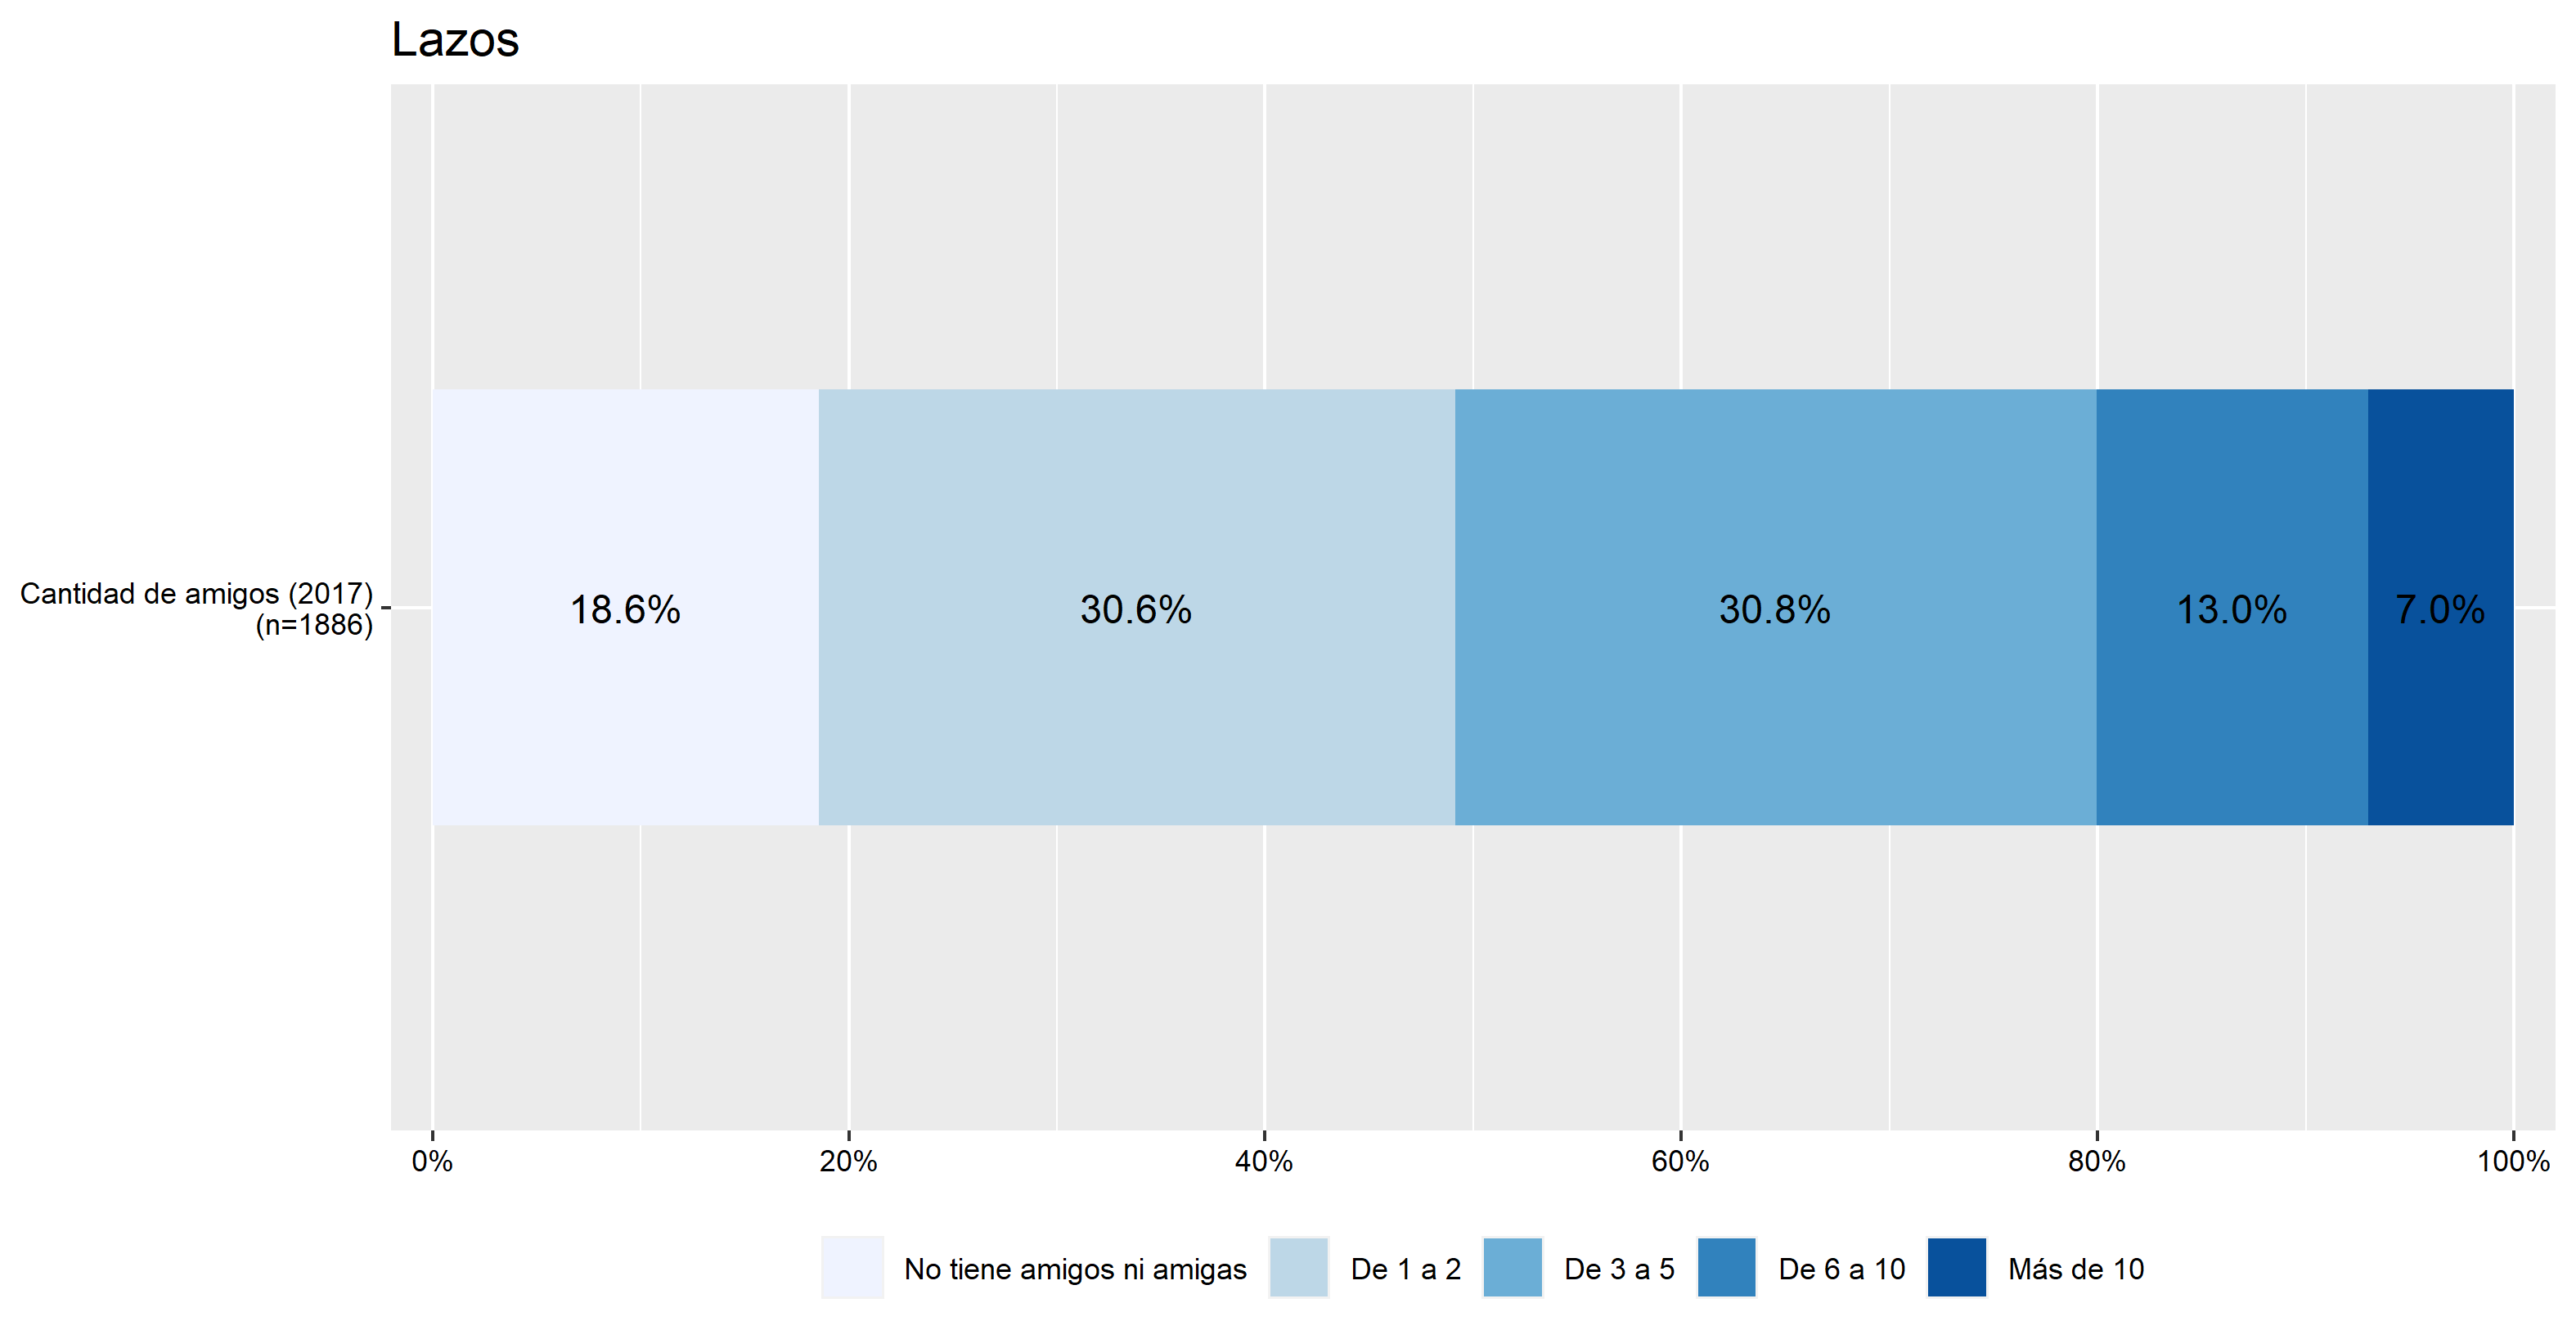
\includegraphics[width=1\linewidth,height=1\textheight]{output/graphs/lazos} 

}

\caption{Item subdimension Lazos.}\label{fig:lazos}
\end{figure}

\begin{figure}[H]

{\centering 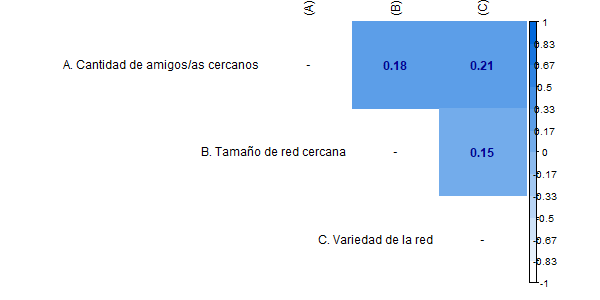
\includegraphics[width=1\linewidth,height=1\textheight]{output/graphs/lazos_cor} 

}

\caption{Asociación de indicadores lazos.}\label{fig:lazos-cor}
\end{figure}

En la matriz de correlaciones de la Figura \ref{fig:lazos-cor} se observa que las correlaciones entre los items están en un rango bajo, donde los items que presentan una correlación mayor son A y C. Para calcular la consistencia interna de estos tres items se utilizó alpha de Cronbach, obteniendo un resultado de 0.32, muy por debajo del valor mínimo recomendado de 0.7. Por lo tanto, para esta subdimensión se decide considerar solo el item ``Cantidad de personas que se conocen con diferentes ocupaciones'' (variedad de la red). Este indicador posee mayor sentido en el marco de la cohesión social, ya que esta va más allá de la calidad y cantidad de lazos cercanos como familia y amigos, contemplando aquellos lazos sociales más extensos.

\hypertarget{sentido-de-pertenencia}{%
\section{Sentido de pertenencia}\label{sentido-de-pertenencia}}

Una segunda dimensión de la definición propuesta por la CEPAL para cohesión social corresponde al sentido de pertenencia, que ``alude a la vinculación e identificación de las personas respecto a la sociedad y a las instituciones y grupos que los integran. Incluye los niveles micro, meso y macro.'' (\protect\hyperlink{ref-cepal_cohesion_2021}{CEPAL, 2021, p. 45}). Esta definición permite relevar la importancia de ``las dinámicas de reconocimiento y participación social para conducir procesos dinámicos de inclusión que contribuyan a la cohesión social y al logro del bienestar (véase, por ejemplo, Jenson, 1998; Kymlicka, 1998)'' (\protect\hyperlink{ref-cepal_cohesion_2021}{CEPAL, 2021, p. 45}). Las subdimensiones que conforman esta dimensión son identificación con el país, percepción de justicia distributiva y confianza institucional.

\textbf{Identificación con el país}

Por medio de esta subdimensión se busca cuantificar la identificación de los individuos ``con los valores y acciones que representan sus instituciones, y la concordancia con los propios'' (\protect\hyperlink{ref-cepal_cohesion_2021}{CEPAL, 2021, p. 66}).

En la propuesta regional de la CEPAL se incluyen los indicadores ``Orgullo por el sistema político'', que busca medir la adhesión de los encuestados con la labor que realizan sus instituciones en la representación de sus valores y objetivos y ``Orgullo por su nacionalidad'', que busca cuantificar la identificación de los encuestados con los valores y normas que rigen las instituciones del país. Al trabajar con ELSOC se utilizan los items ``Orgullo de ser chileno'' e ``Identificación con Chile'', presentes en las cinco olas del estudio. Un análisis descriptivo de estos items se presenta en la Figura \ref{fig:identificacion}.

\begin{figure}[H]

{\centering 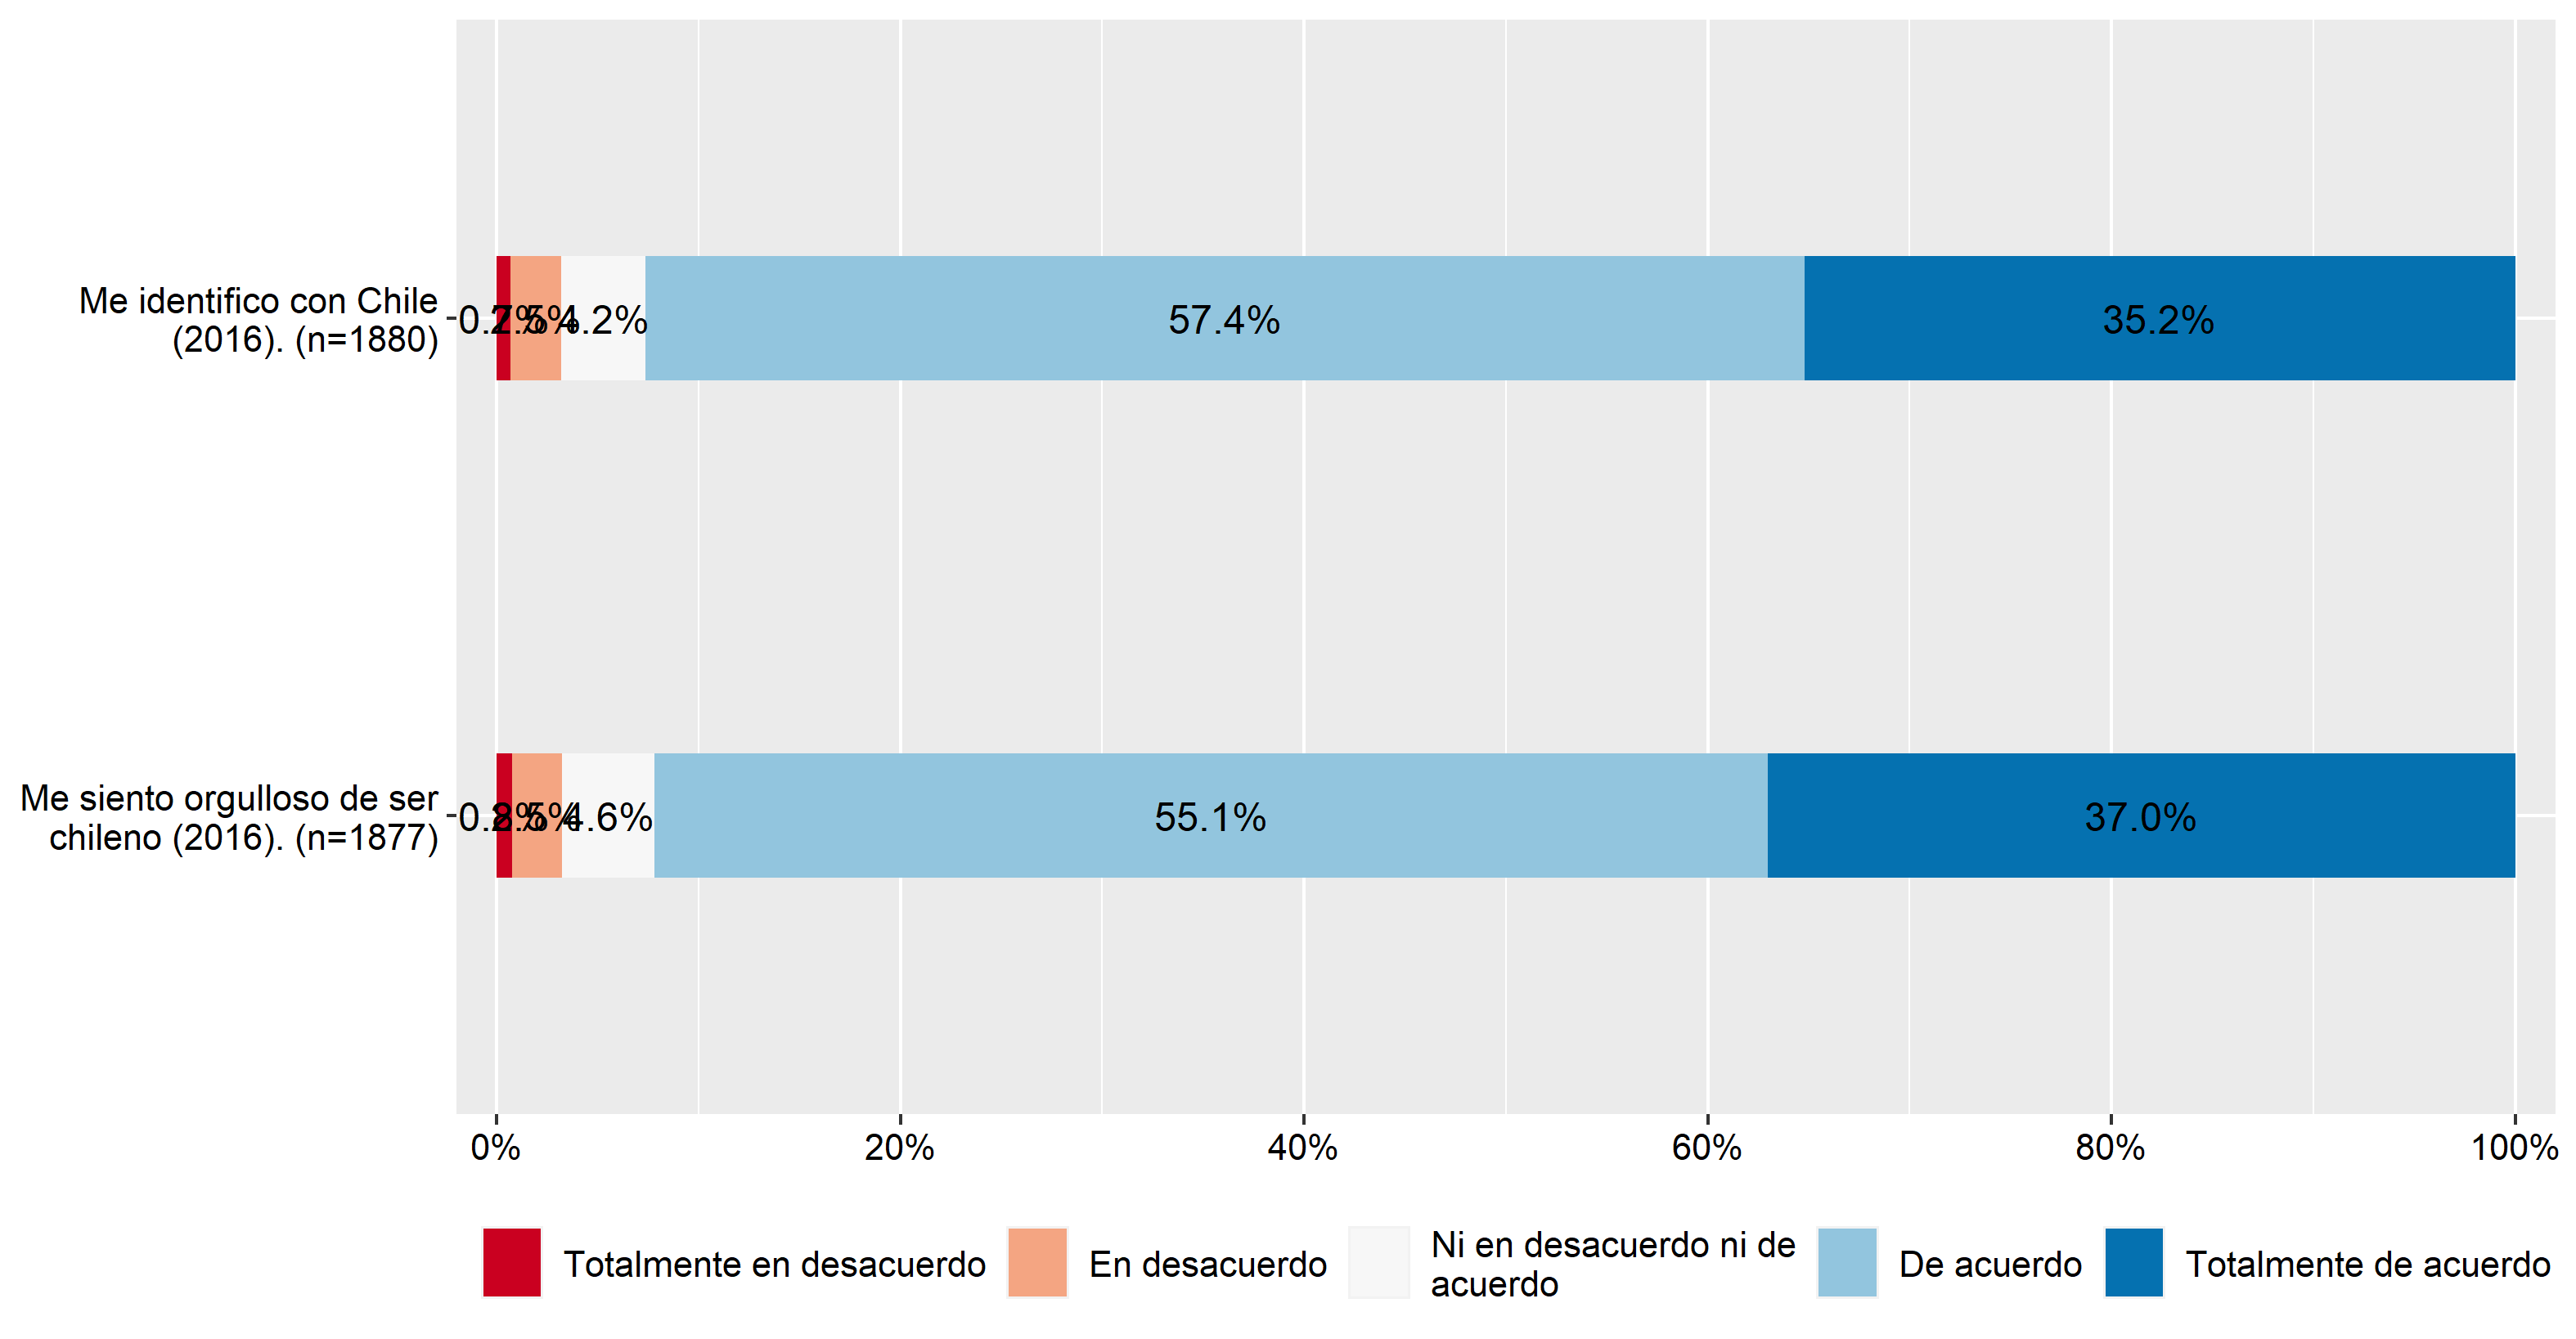
\includegraphics[width=1\linewidth,height=1\textheight]{output/graphs/identificacion} 

}

\caption{Identificación y orgullo con Chile.}\label{fig:identificacion}
\end{figure}

La correlación entre estos items es positiva y alta (r=0.77). Por lo tanto, en esta subdimensión se utilizará como índicador un promedio simple de ambos items.

\textbf{Percepción de justicia}

La subdimensión de percepción de justicia refiere al examen que realizan las personas respecto a la capacidad de las instituciones de entregar bienestar y/o distribuir el poder económico y político (\protect\hyperlink{ref-cepal_cohesion_2021}{CEPAL, 2021}).

En la propuesta regional de la CEPAL se utilizan los indicadores ``Se deben equiparar los sueldos, no mantener desigualdad para incentivar el esfuerzo personal'', que cuantifica percepciones respecto a aversiones hacia la desigualdad; ``El trabajo a largo plazo da beneficios, no las conexiones o suerte'', que busca captar percepciones sobre la estructura de oportunidades en el país y las expectativas de movilidad social; y ``El Estado debe implementar políticas para reducir la desigualdad de ingreso'', que aborda las percepciones respecto a la desigualdad de ingresos en el país. Al trabajar con ELSOC se utilizan los items ``En Chile las personas son recompensadas por su esfuerzo'' y ``En Chile las personas son recompensadas por su inteligencia'', presentes en todas las olas. Un gráfico descriptivo de estos items se presenta en la Figura \ref{fig:justicia}.

\begin{figure}[H]

{\centering 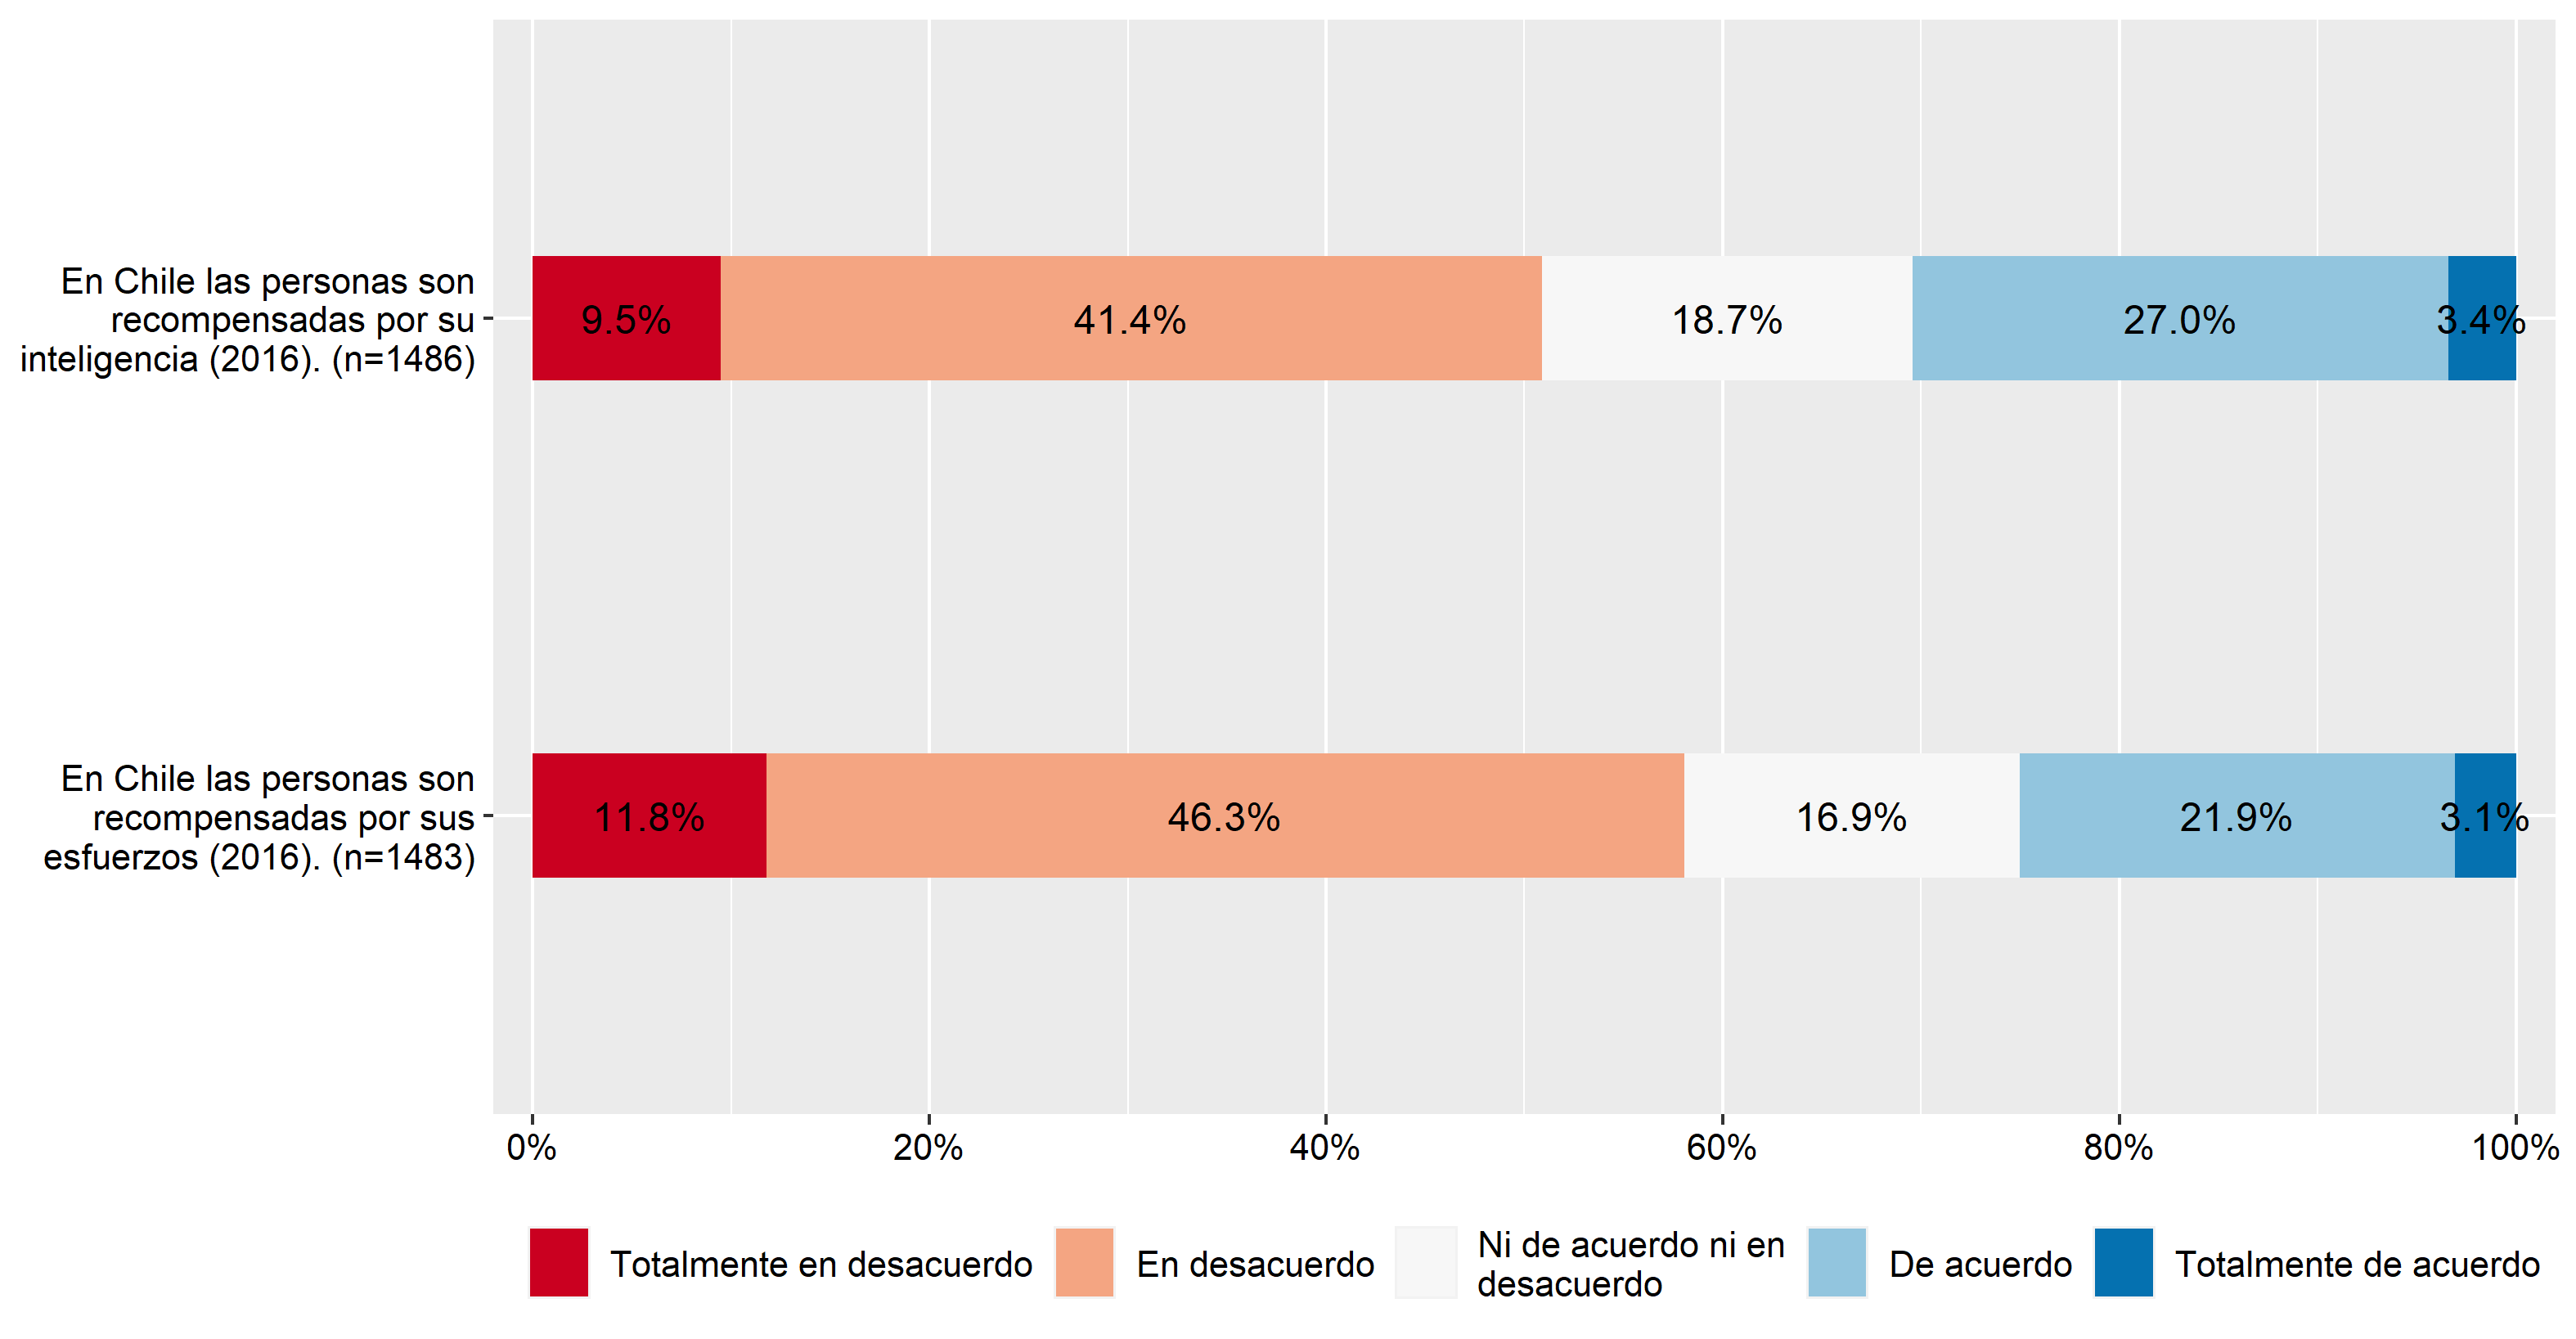
\includegraphics[width=1\linewidth,height=1\textheight]{output/graphs/justicia} 

}

\caption{Descriptivos Percepción de recompensa por esfuerzo e inteligencia.}\label{fig:justicia}
\end{figure}

La correlación entre estos items es positiva y alta (r=0.7). Por lo tanto, se utilizará como índice un promedio simple de ambos items en esta subdimensión.

\textbf{Confianza institucional}

La subdimensión de confianza institucional ``mide la valoración implícita de las acciones llevadas a cabo por las instituciones para representar los valores de la sociedad y/o de orientar la acción hacia el bien colectivo (Warren, 2010)'' (\protect\hyperlink{ref-cepal_cohesion_2021}{CEPAL, 2021, p. 66}).

En la propuesta regional de la CEPAL se utiliza grado de confianza en (a) las cortes, (b) el Congreso Nacional, (c) la Policía Nacional, (d) los partidos políticos, (e) el ejecutivo y (f) las elecciones. Al trabajar con ELSOC se utilizan los siguientes ocho items presentes en las cinco olas: grado de confianza en (a) el gobierno, (b) los partidos políticos; (c) carabineros; (d) los sindicatos; (e) el poder judicial; (f) las empresas privadas; (g) el congreso nacional; y (h) el presidente/a de la república. Un análisis descriptivo de estos items se presenta en la Figura \ref{fig:confianza-institucional} y la estimación de las correlaciones en la Figura \ref{fig:confianza-institucional-cor}.

\begin{figure}[H]

{\centering 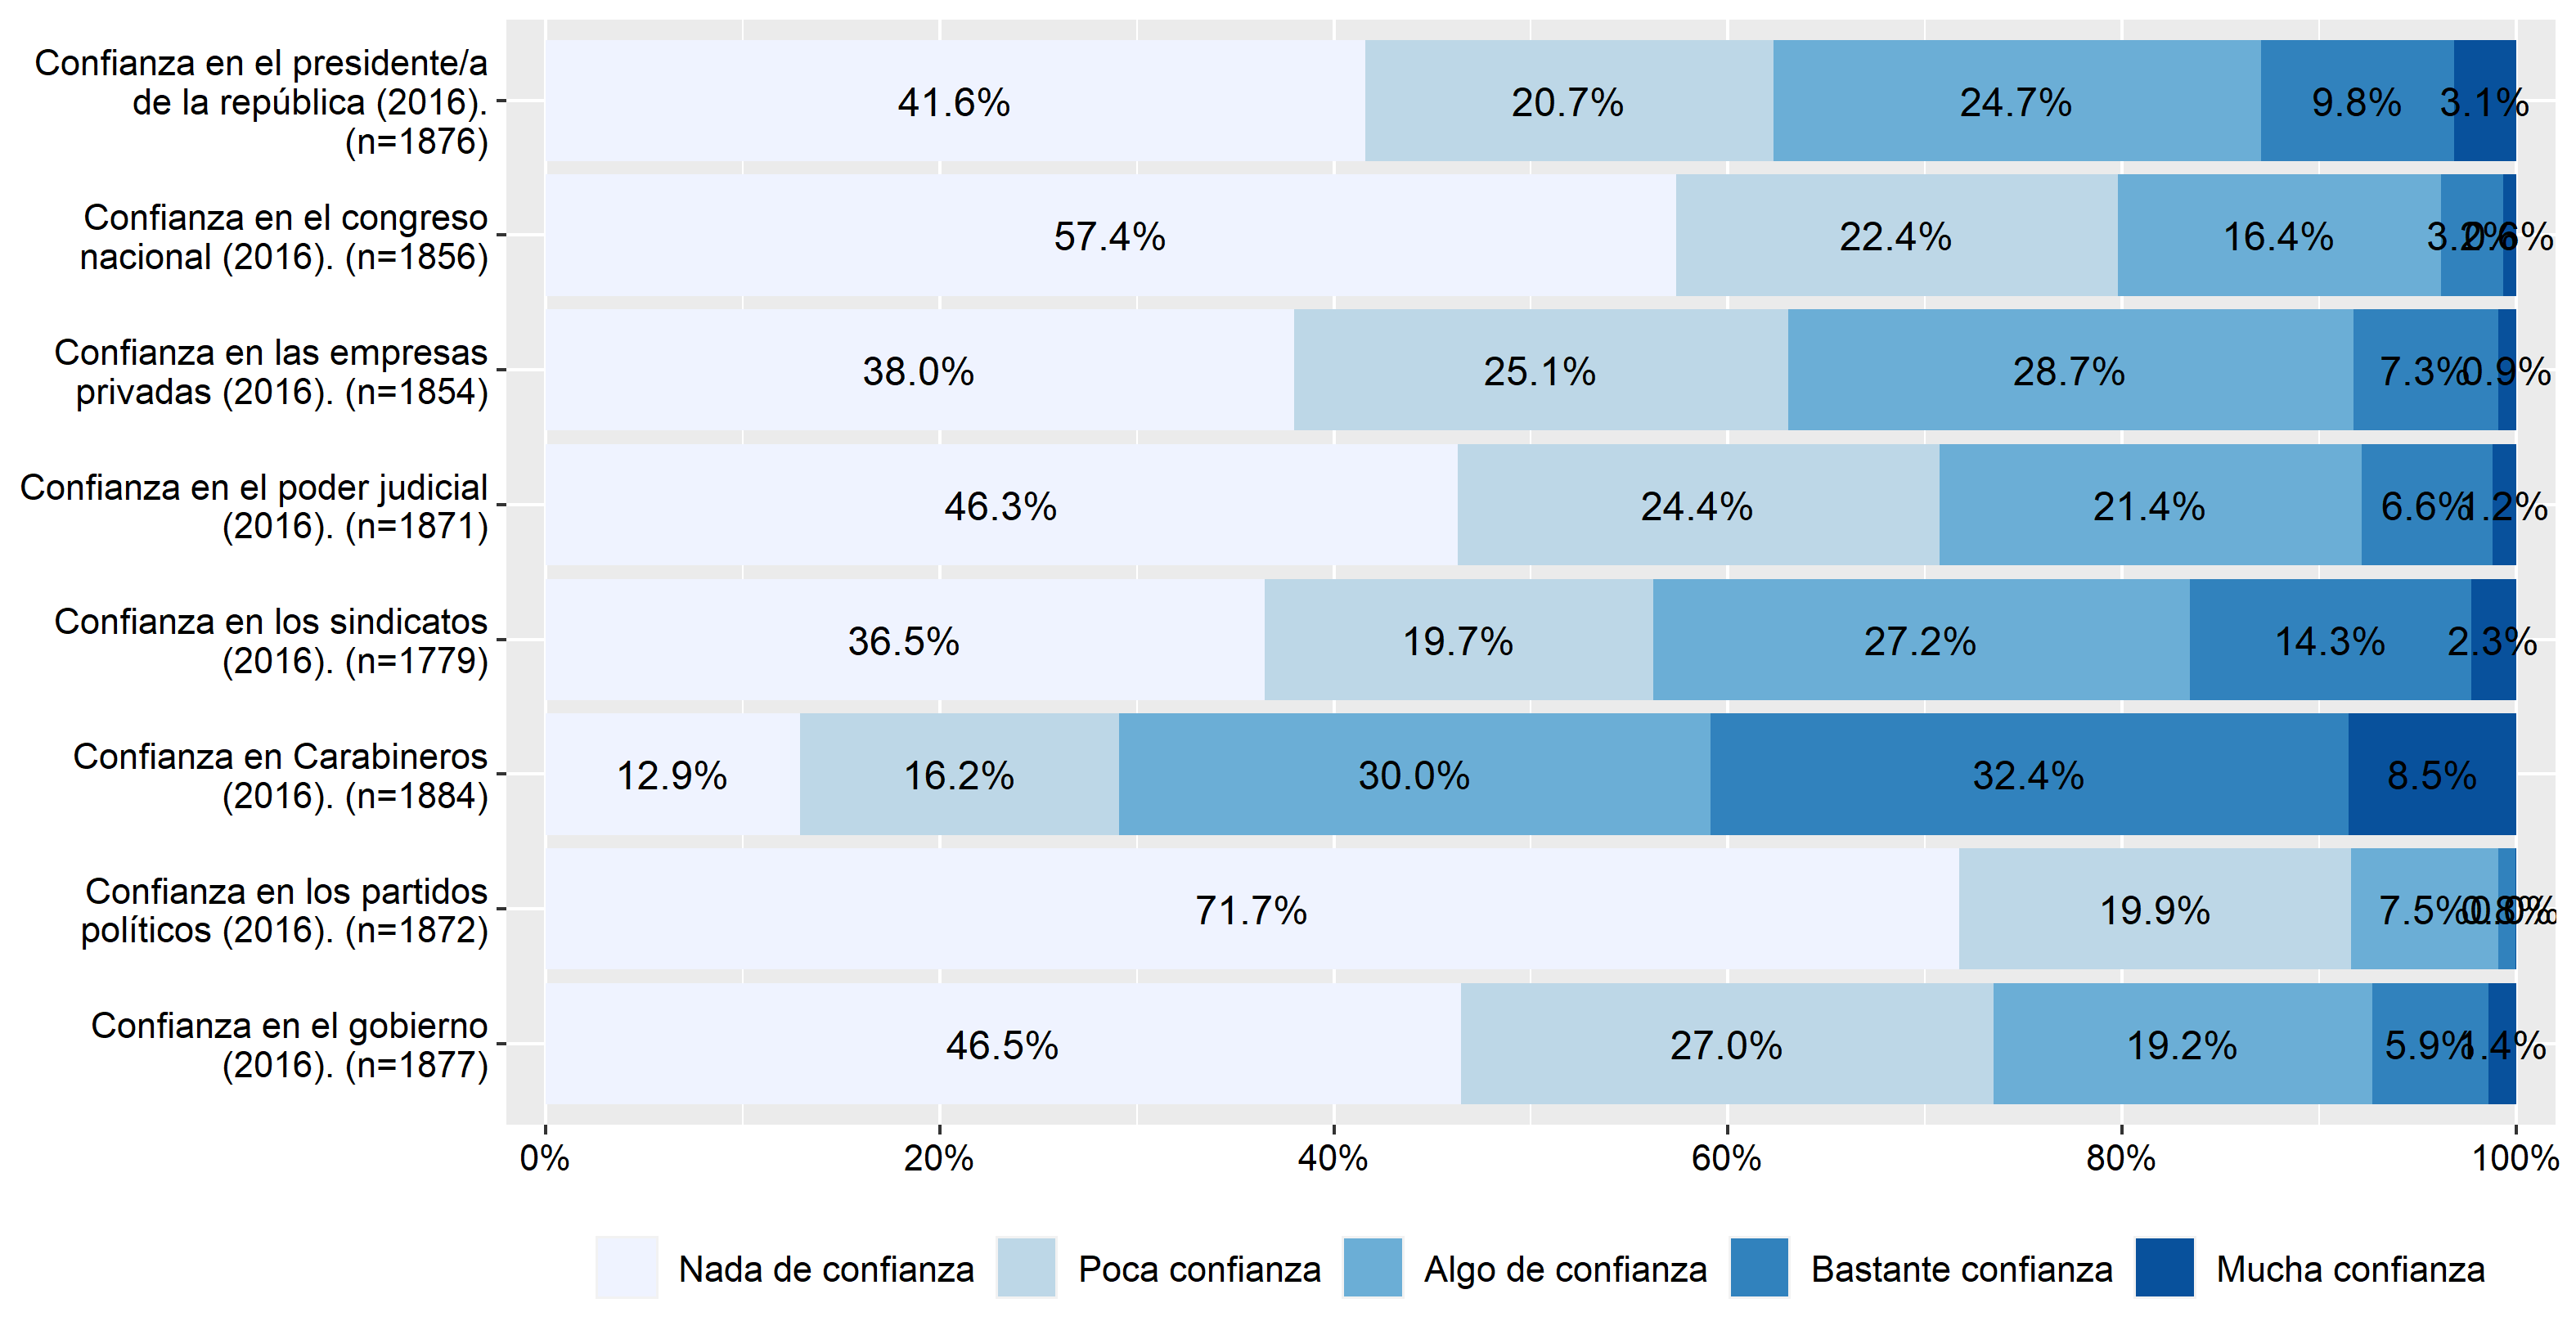
\includegraphics[width=1\linewidth,height=1\textheight]{output/graphs/confianza-institucional} 

}

\caption{Confianza en instituciones.}\label{fig:confianza-institucional}
\end{figure}

\begin{figure}[H]

{\centering 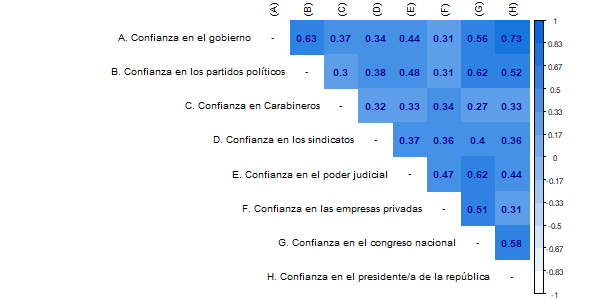
\includegraphics[width=1\linewidth,height=1\textheight]{output/graphs/confianza-institucional_cor} 

}

\caption{Asociación indicadores Confianza institucional.}\label{fig:confianza-institucional-cor}
\end{figure}

En esta oportunidad, nuevamente se utilizó un análisis factorial exploratorio con el objetivo de construir un indicador a partir de la información de las dimensiones comunes que subyacen a este conjunto de ocho items. La Tabla \ref{tab:inst-fa} muestra el resultado de la extracción de tres factores:

\begin{longtable}[]{@{}l@{}}
\caption{\label{tab:inst-fa}Dimensiones de confianza institucional.}\tabularnewline
\toprule
\endhead

\includegraphics[width=8.33333in,height=\textheight]{output/tables/inst_fa.png} \\
\bottomrule
\end{longtable}

En la Tabla \ref{tab:inst-fa} observamos en la segunda columna (ML1) un factor que se relaciona con las preguntas sobre el grado de confianza con instituciones políticas (el gobierno, presidente/a, partidos políticos), luego un segundo factor (ML2) que se asocia con el poder judicial y el congreso, y finalmente un tercer factor (ML3) asociado con empresas privadas, carabineros, sindicatos y poder judicial. En relación con la varianza asociada a estos tres factores, el primer factor representa un 20\% de la varianza y los otros dos un 15\%. Por lo tanto, existe cierto grado de consistencia en los tres factores, siendo el primero de ellos -relacionado con las instituciones políticas- el que representa una mayor proporción de la varianza y por tanto el indicador de confianza institucional incluirá estos tres items.

\hypertarget{orientaciuxf3n-hacia-el-bien-comuxfan}{%
\section{Orientación hacia el bien común}\label{orientaciuxf3n-hacia-el-bien-comuxfan}}

Esta tercera dimensión refiere a ``una actitud favorable a acciones que propendan a un mayor bienestar colectivo versus el beneficio puramente individual como parte de un proyecto compartido, o bien, como indican Sorj y Tironi (2007), aceptar ``vivir en un orden colectivo que les reportará beneficios, así como sacrificios individuales.'' (\protect\hyperlink{ref-cepal_cohesion_2021}{CEPAL, 2021, p. 46})

\textbf{Solidaridad}

La subdimensión de solidaridad busca cuantificar la presencia de valores solidarios en los individuos. Esta solidaridad se basa en el ``entendimiento de la reciprocidad aprendida en redes, y es un reflejo de la solidaridad que perciben recibir por parte del Estado y sus pares (CEPAL, 2007)'' (\protect\hyperlink{ref-cepal_cohesion_2021}{CEPAL, 2021, p. 66}).

En el informe de la CEPAL se utiliza como indicador el item ``Asistencia a reuniones de un grupo de mejoras para la comunidad''. Al trabajar con ELSOC se utilizará este item y otros siete que abordan un comportamiento prosocial y que se encuentran en las cinco olas. Estos items se describen en la Figura \ref{fig:solidaridad} y un análisis bivariado se muestra en la Figura \ref{fig:solidaridad-cor}.

\begin{figure}[H]

{\centering 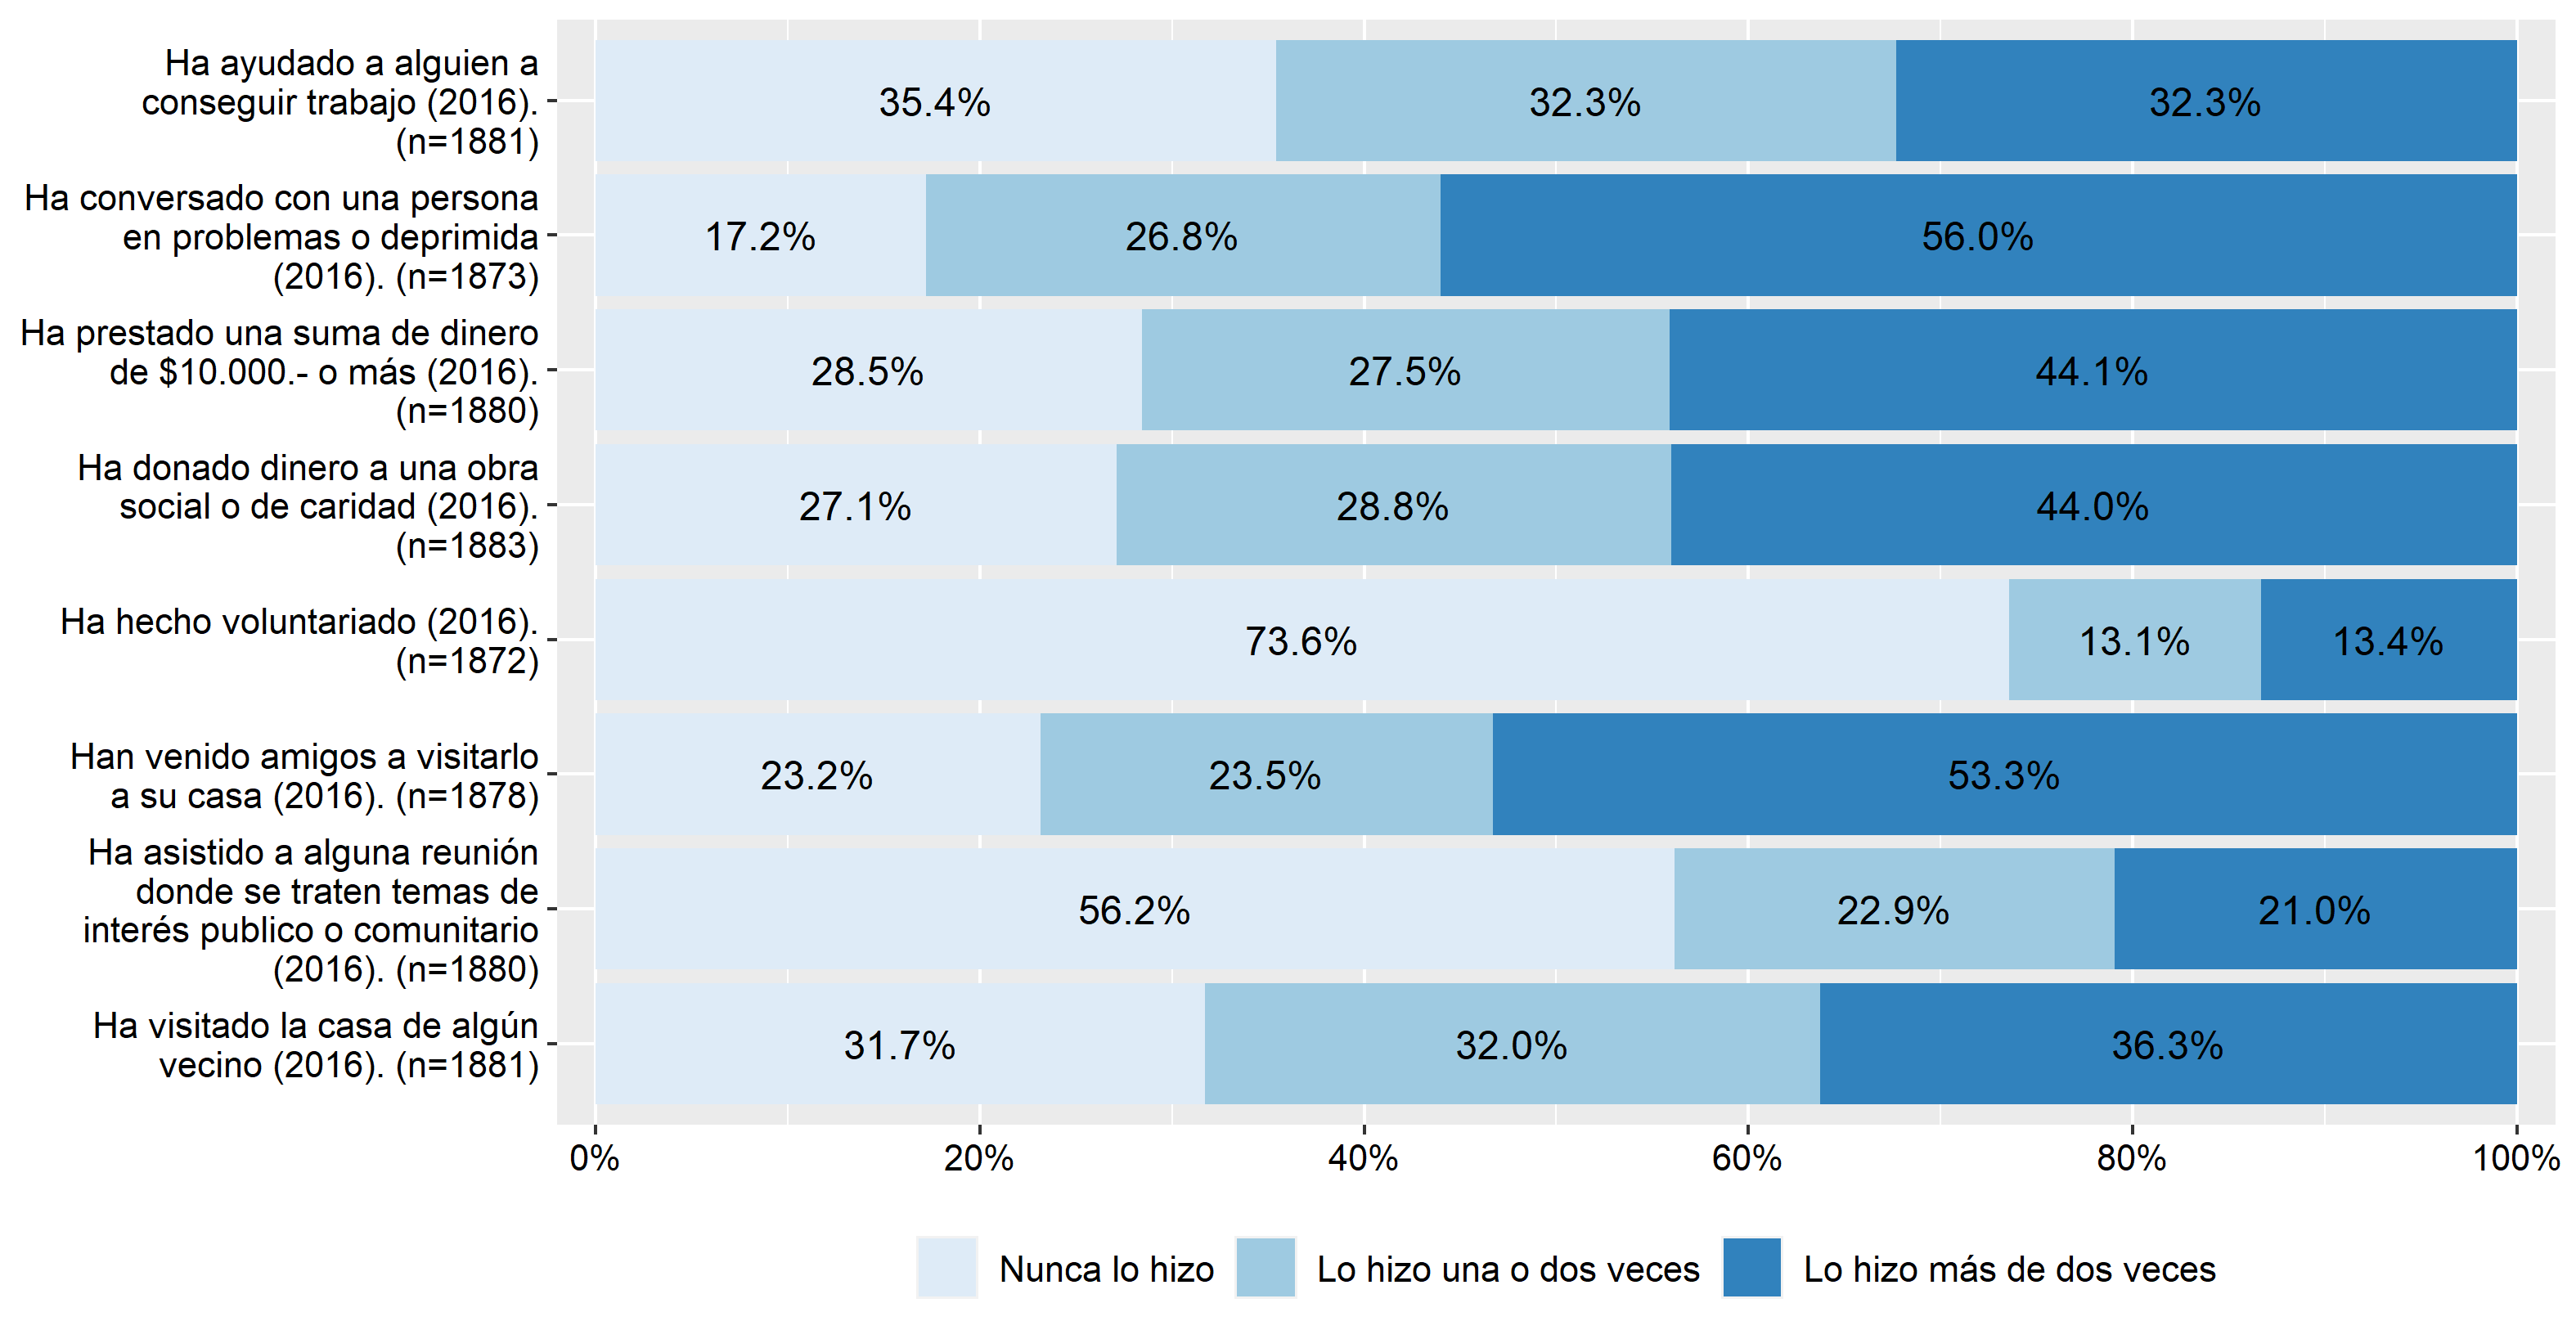
\includegraphics[width=1\linewidth,height=1\textheight]{output/graphs/solidaridad} 

}

\caption{Acciones de solidaridad.}\label{fig:solidaridad}
\end{figure}

\begin{figure}[H]

{\centering 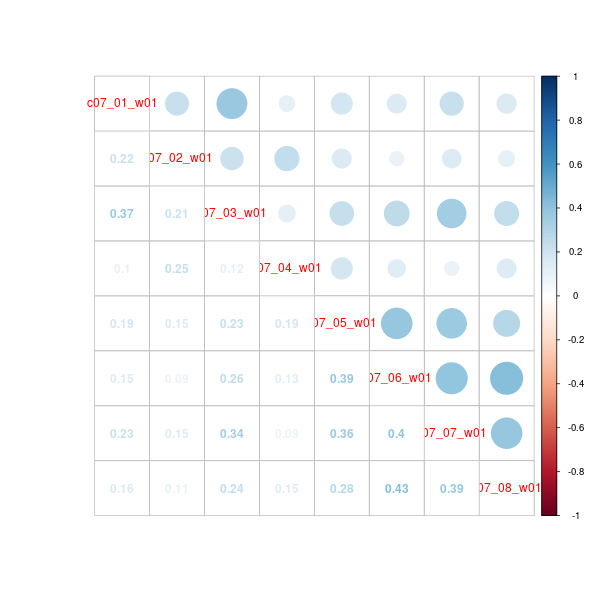
\includegraphics[width=1\linewidth,height=1\textheight]{output/graphs/solidaridad_cor} 

}

\caption{Asociación indicadores de solidaridad.}\label{fig:solidaridad-cor}
\end{figure}

Como esta subdimensión posee ocho items, se volvió a realizar un análisis factorial exploratorio para construir un índice a partir de la información de las dimensiones comunes entre este conjunto de items. La Tabla \ref{tab:solidaridad-fa} muestra el resultado de la extracción de tres factores:

\begin{longtable}[]{@{}l@{}}
\caption{\label{tab:solidaridad-fa}Dimensiones de solidaridad.}\tabularnewline
\toprule
\endhead

\includegraphics[width=8.33333in,height=\textheight]{output/tables/solidaridad_fa.png} \\
\bottomrule
\end{longtable}

En la Tabla \ref{tab:inst-fa} se observa en la segunda columna (ML2) un factor relacionado con acciones de solidaridad como prestar o donar dinero, ayudar a una persona a conseguir trabajo y conversar con una persona con problemas o deprimida, luego en la tercera columna (ML1) se observa un tercer factor que posee un item sobre realizar trabajo voluntario. Finalmente, en la cuarta columna (ML3) se presenta un factor asociado con la participación en reuniones sociales, como visitar casas de vecinos, recibir visitas de amigos o asistir a reuniones donde se traten problemas relevantes para la comunidad. En relación con la varianza que se asocia a cada uno de estos factores, el primer factor representa un 18\% de la varianza, el segundo un 13\% y el tercero un 12\%. Por lo tanto, se propone utilizar un indicador asociado al primer factor que incluye los items ``Ha prestado una suma de dinero de \$10.000.- o más'', ``Ha ayudado a alguien a conseguir trabajo'', ``Ha conversado con una persona en problemas o deprimida'' y ``Ha donado dinero a una obra social o de caridad''.

\textbf{Participación cívica}

La subdimensión de participación cívica da cuenta de la voluntad de adherir a los espacios de participación del sistema político y la vinculación de los individuos con su comunidad. Esta subdimensión ``promueve la participación ciudadana en los asuntos públicos, apoyando proyectos colectivos que representen sus opiniones o intereses políticos (Valdéz, Viramontes y Finol, 2016)'' (\protect\hyperlink{ref-cepal_cohesion_2021}{CEPAL, 2021, p. 66}).

En informe CEPAL se utilizaron los indicadores ``Tiene actividad política (firma peticiones, boicot, va a manifestaciones pacíficas, huelgas)'', que indica la predisposición hacia la actividad política, ``Participación en organizaciones'', que busca medir la implicación de los individuos con su comunidad y ``Voto en elecciones presidenciales'', que pretende capturar el grado de compromiso cívico con el sistema regente y la dirección de la sociedad. Al trabajar con ELSOC se utilizan cuatro items de actividad política presentes en las cuatro primeras olas, ocho items de participación en organizaciones presentes en ola 2016 y 2018 y voto en elecciones 2013 y 2017 (ola 2016 y 2018). Un gráfico descriptivo de estos items se presenta en la Figura \ref{fig:participacion-civica}, en la Figura \ref{fig:participacion-organizaciones} y en la Figura \ref{fig:participacion-electoral}, mientras que las correlaciones se muestran en la Figura \ref{fig:participacion-civica-cor} y en la Figura \ref{fig:participacion-organizaciones-cor}. La tasa de respuesta considera un N de alrededor de 1490 respuestas.

\begin{figure}[H]

{\centering 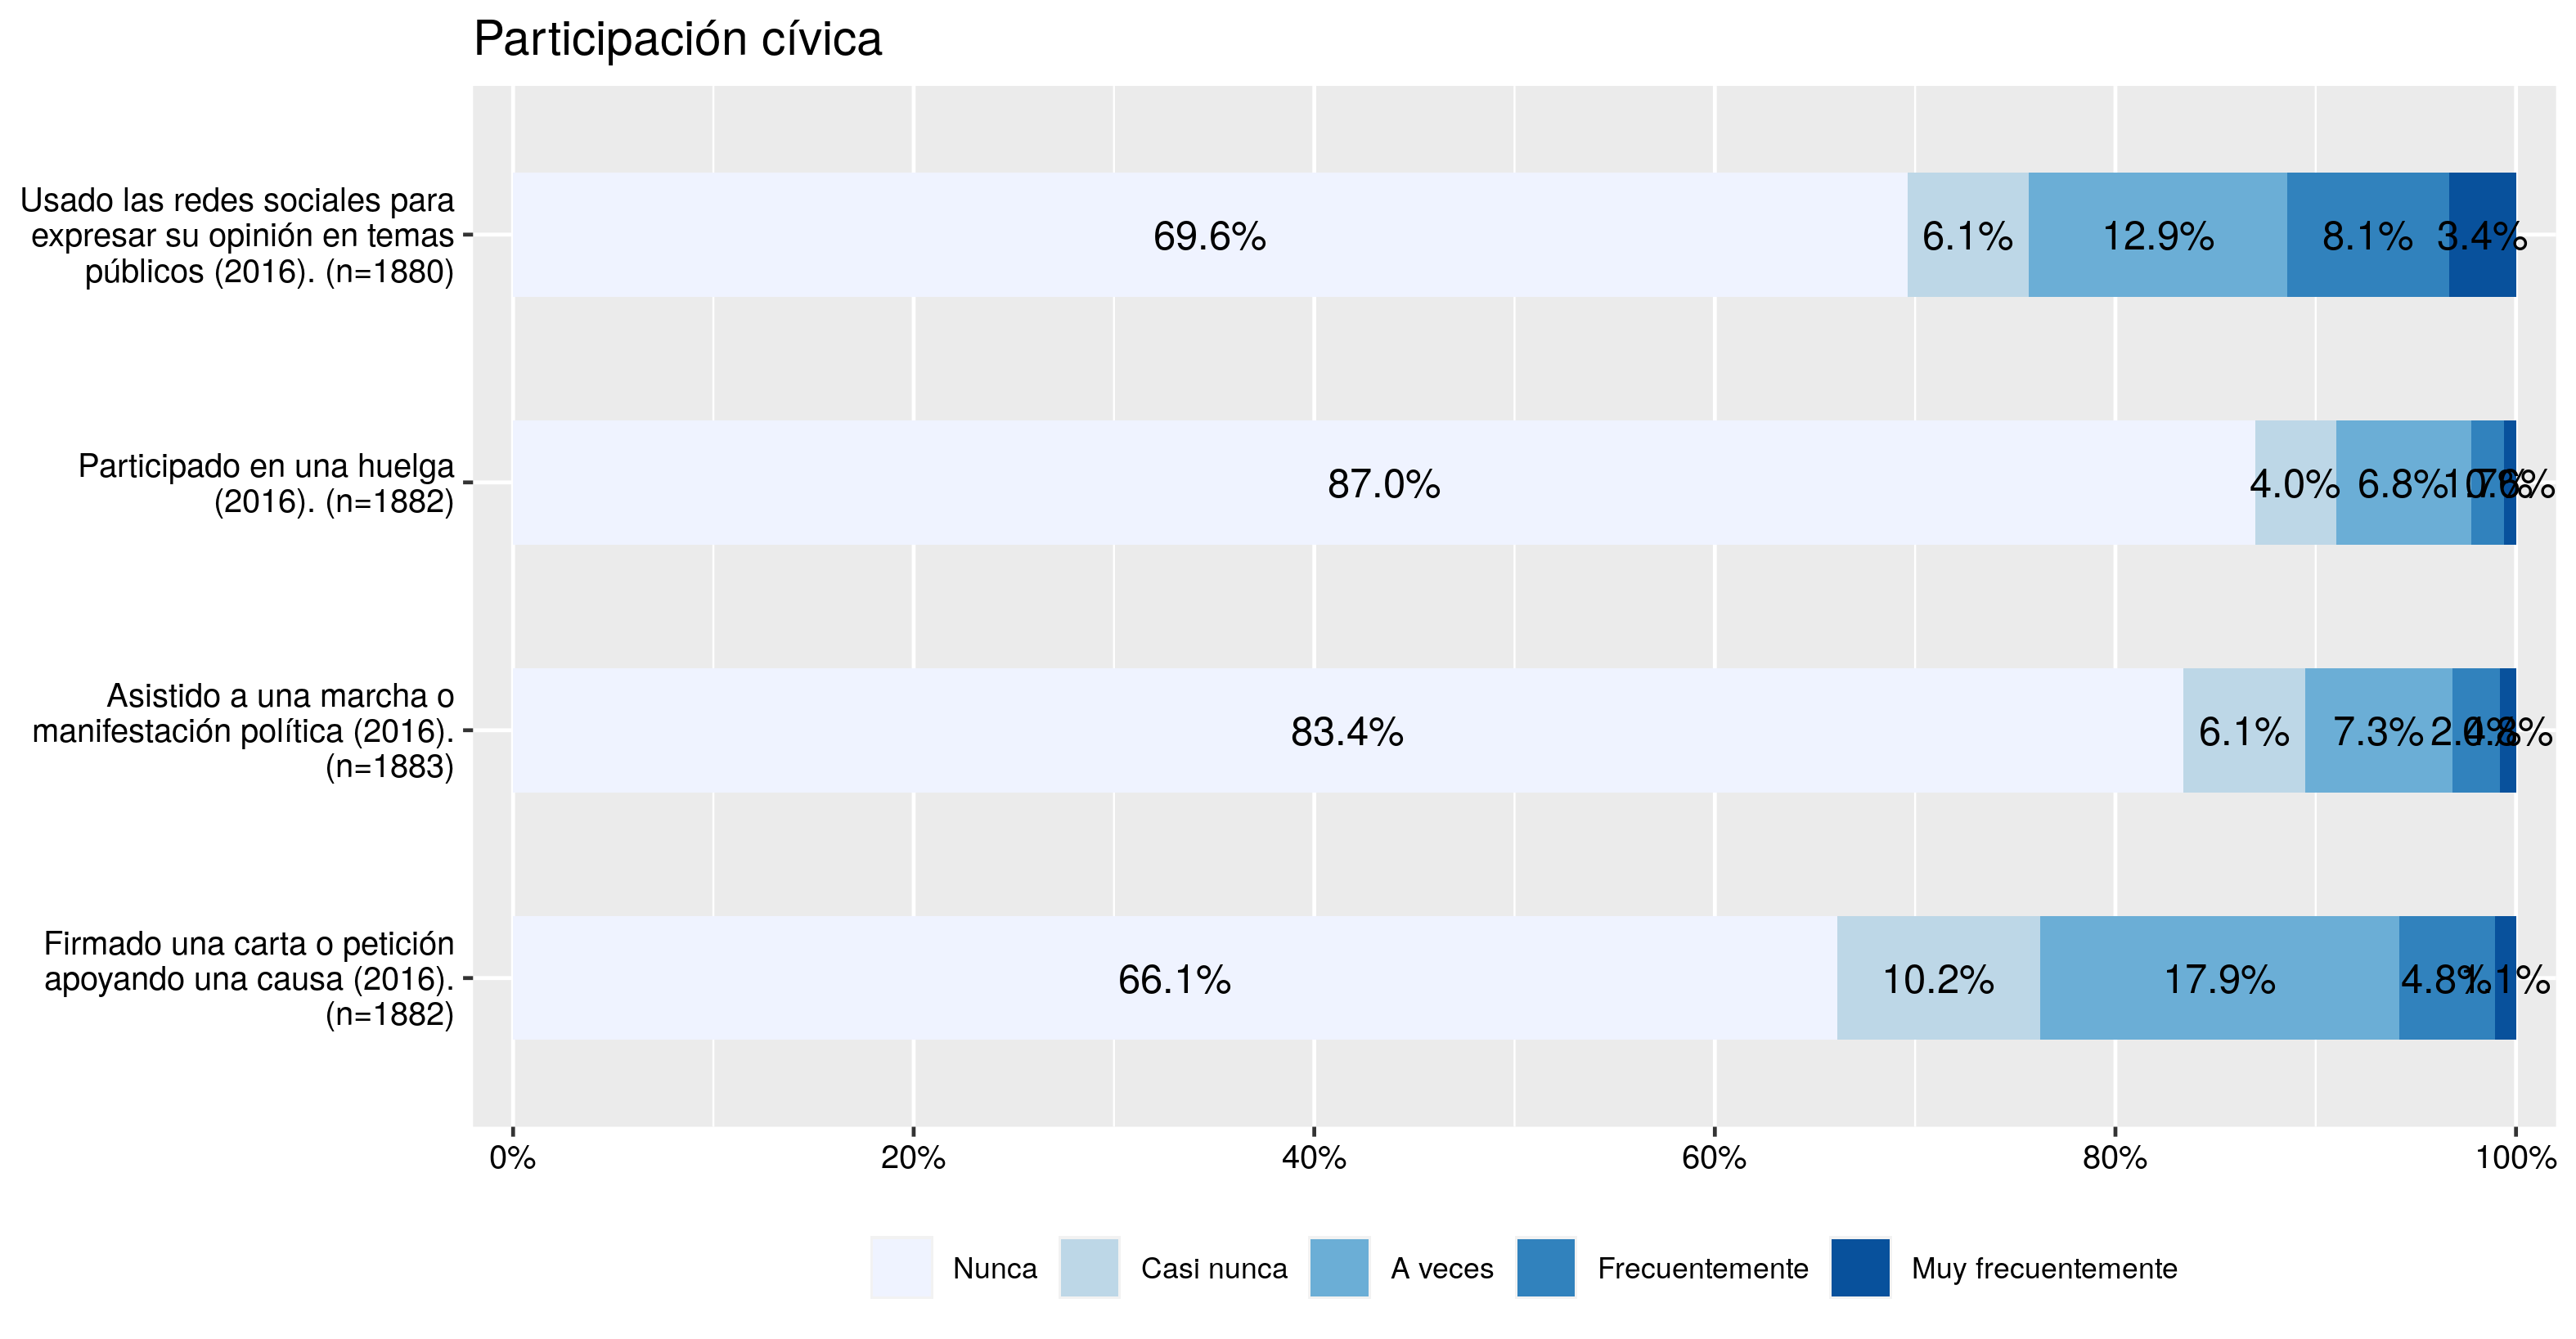
\includegraphics[width=1\linewidth,height=1\textheight]{output/graphs/participacion-civica} 

}

\caption{Participación en actividades cívicas.}\label{fig:participacion-civica}
\end{figure}

\begin{figure}[H]

{\centering 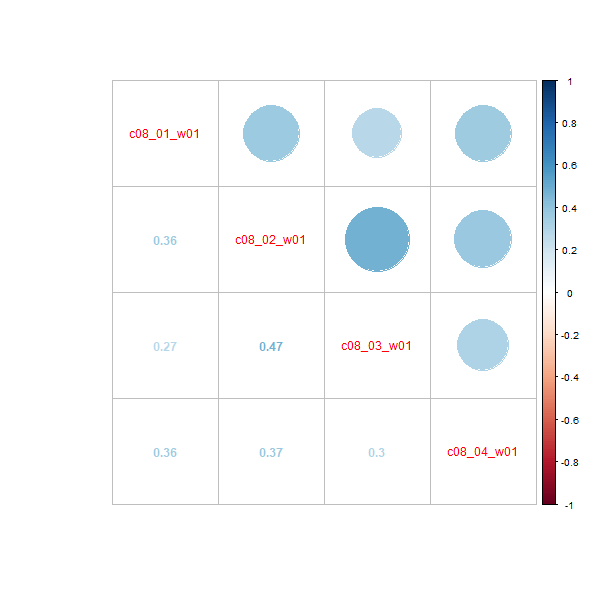
\includegraphics[width=1\linewidth,height=1\textheight]{output/graphs/participacion-civica_cor} 

}

\caption{Asociación indicadores participación cívica.}\label{fig:participacion-civica-cor}
\end{figure}

\textbf{Participación en organizaciones}

\begin{figure}[H]

{\centering 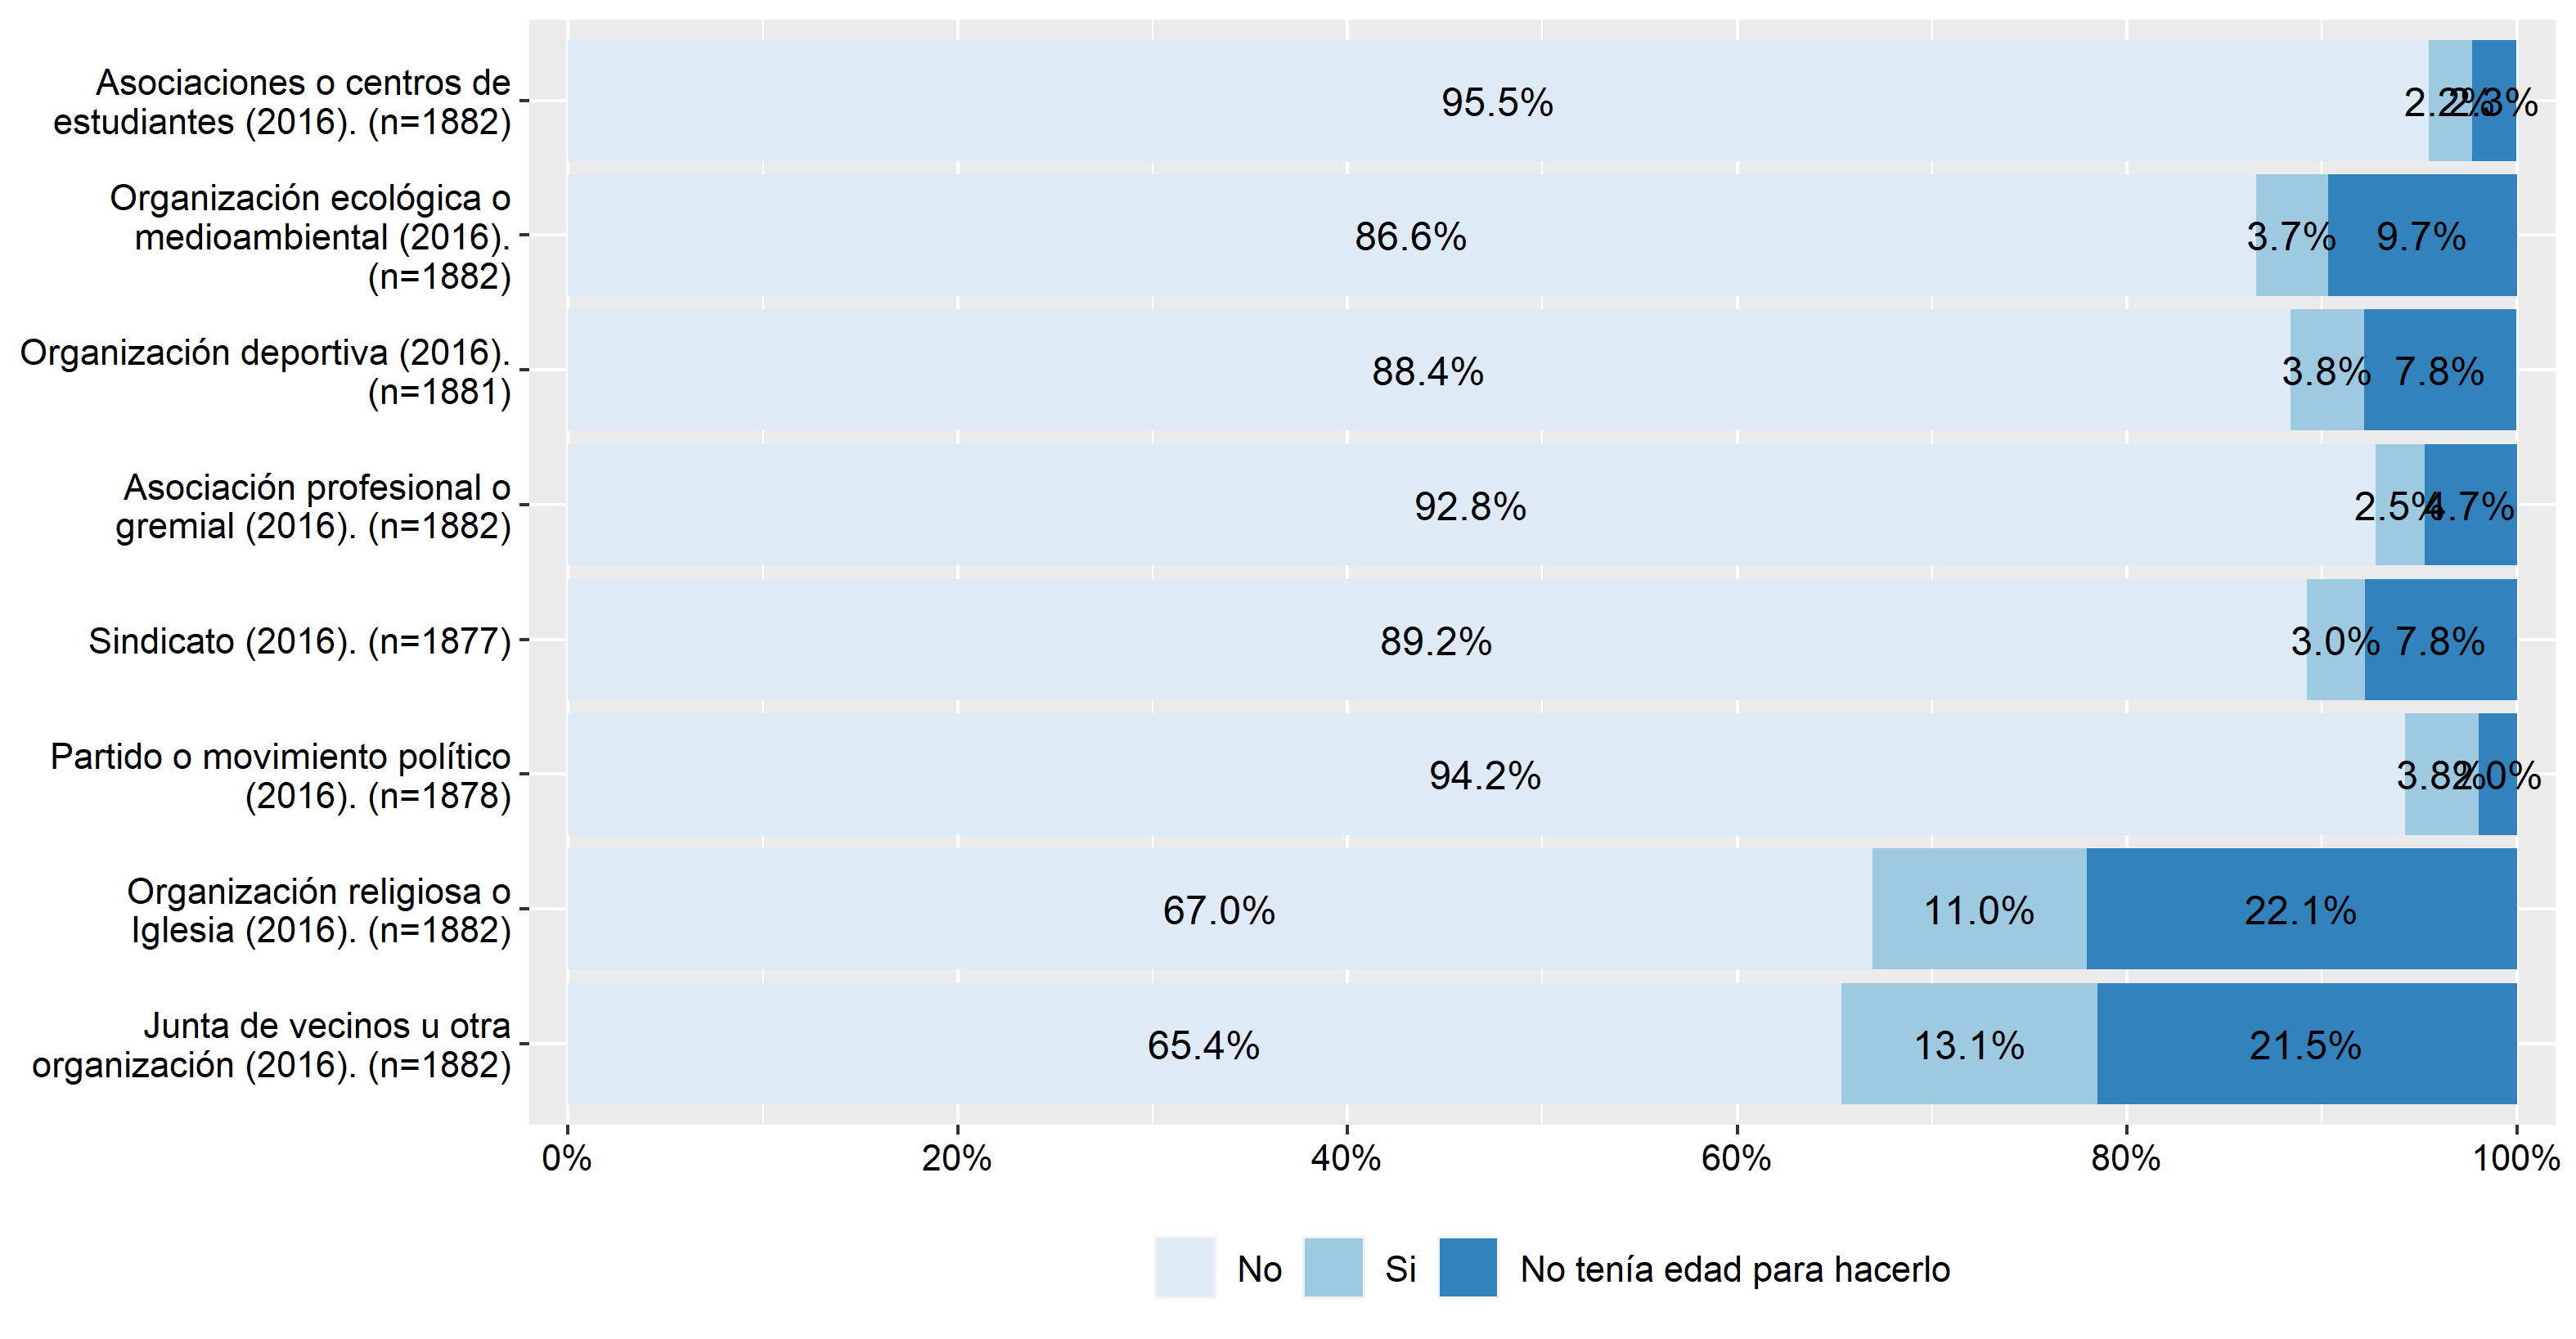
\includegraphics[width=1\linewidth,height=1\textheight]{output/graphs/participacion-organizaciones} 

}

\caption{Participación en organizaciones sociales.}\label{fig:participacion-organizaciones}
\end{figure}

\begin{figure}[H]

{\centering 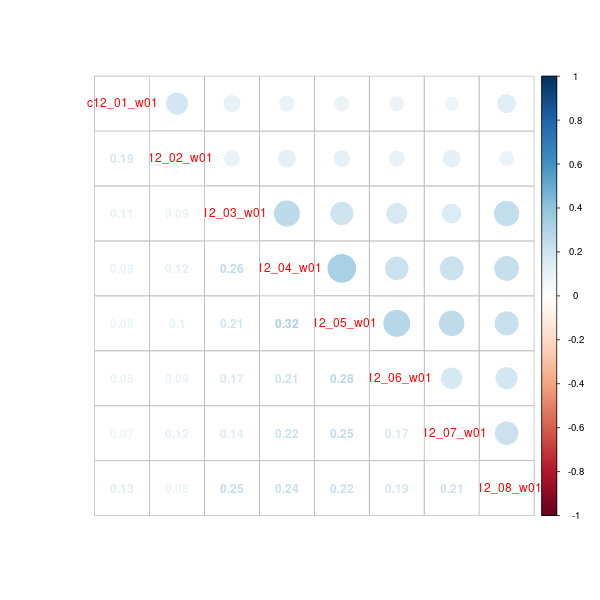
\includegraphics[width=1\linewidth,height=1\textheight]{output/graphs/participacion-organizaciones_cor} 

}

\caption{Asociación indicadores participación en organizaciones.}\label{fig:participacion-organizaciones-cor}
\end{figure}

\textbf{Participación electoral}

\begin{figure}[H]

{\centering 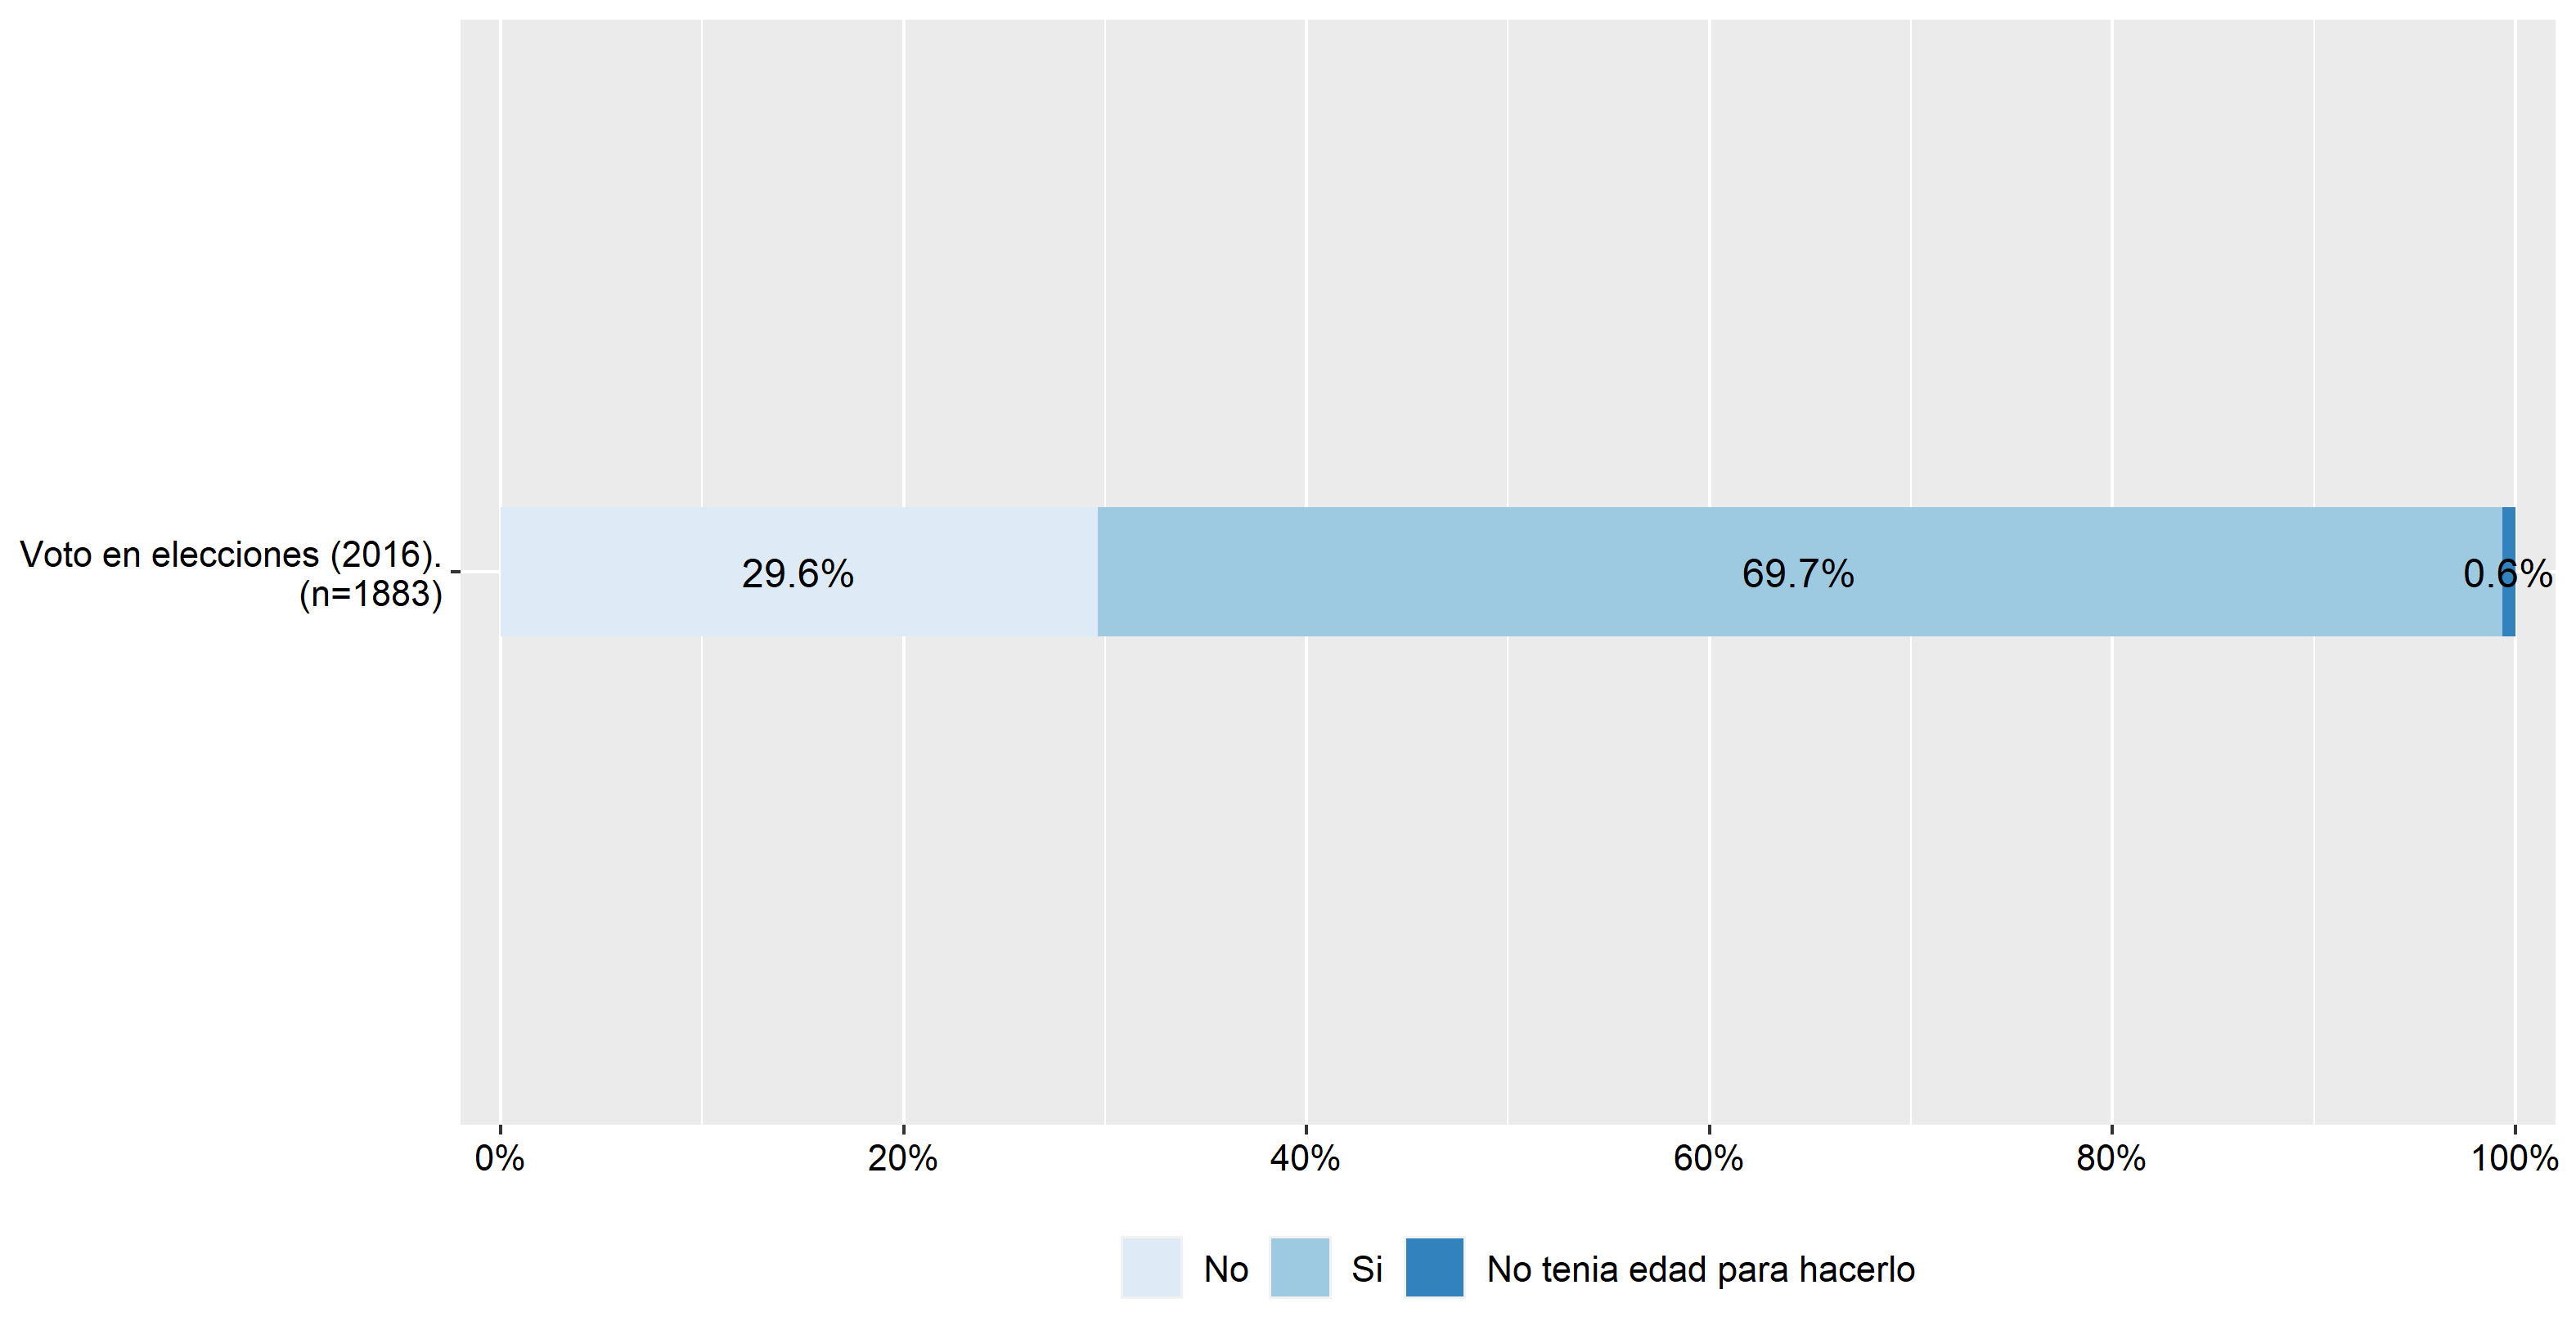
\includegraphics[width=1\linewidth,height=1\textheight]{output/graphs/participacion-electoral} 

}

\caption{Participación en elecciones 2013.}\label{fig:participacion-electoral}
\end{figure}

En esta oportunidad, se utilizó un análisis factorial exploratorio sobre los cuatro items de participación cívica, sobre los ocho tipos de participación en organizaciones presentes en ELSOC y sobre el item de participación en elecciones con el objetivo de construir un índice a partir de la información de las dimensiones comunes que subyacen a este conjunto de items. La Tabla \ref{tab:participacion-fa} muestra el resultado de la extracción de tres factores:

\begin{longtable}[]{@{}l@{}}
\caption{\label{tab:participacion-fa}Dimensiones de Participación cívica y en organizaciones.}\tabularnewline
\toprule
\endhead

\includegraphics[width=8.33333in,height=\textheight]{output/tables/participacion_fa.png} \\
\bottomrule
\end{longtable}

Podemos observar en la Tabla \ref{tab:participacion-fa} un primer factor asociado a la participación cívica (asitir a marchas, participar en huelgas, expresar opiniones por redes sociales y firmar una carta o petición). Luego se observa un segundo factor que incluye la participación en cinco organizaciones (asociación profesional, organización deportiva, sindicato, centro de estudiantes y partidos políticos). Finalmente, se observa un tercer factor que incluye la participación en una organización religiosa y en juntas de vecinos. En cuanto a la varianza asociada a cada uno de estos factores, el primer factor es el más alto, representando un 12\% de la varianza. El segundo y tercer factor representan un 7\% y 6\% respectivamente. Por lo tanto, no existe un grado de consistencia relevante en el segundo y tercer factor, por lo cual se propone no incluir los items asociados a la participación en organizaciones y trabajar solo con los items referentes a participación cívica.

Finalmente, la subdimensión de Respeto por reglas sociales presente en esta dimensión de la propuesta regional de la CEPAL lamentablemente no tiene representación en los items de ELSOC.

\hypertarget{cohesiuxf3n-territorial}{%
\section{Cohesión territorial}\label{cohesiuxf3n-territorial}}

De manera adicional, se incorpora una dimensión sobre calidad de vida en el vecindario presente en ELSOC. Todos estos items se encuentran presentes en las cinco olas.

\textbf{Confianza en vecinos}

En la encuesta ELSOC se incluye un item territorial sobre el grado de confianza en vecinos. Un análisis descriptivo de este item, que sería el único representante de esta subdimensión, se presenta en la Figura \ref{fig:confianza-vecinos}.

\begin{figure}[H]

{\centering 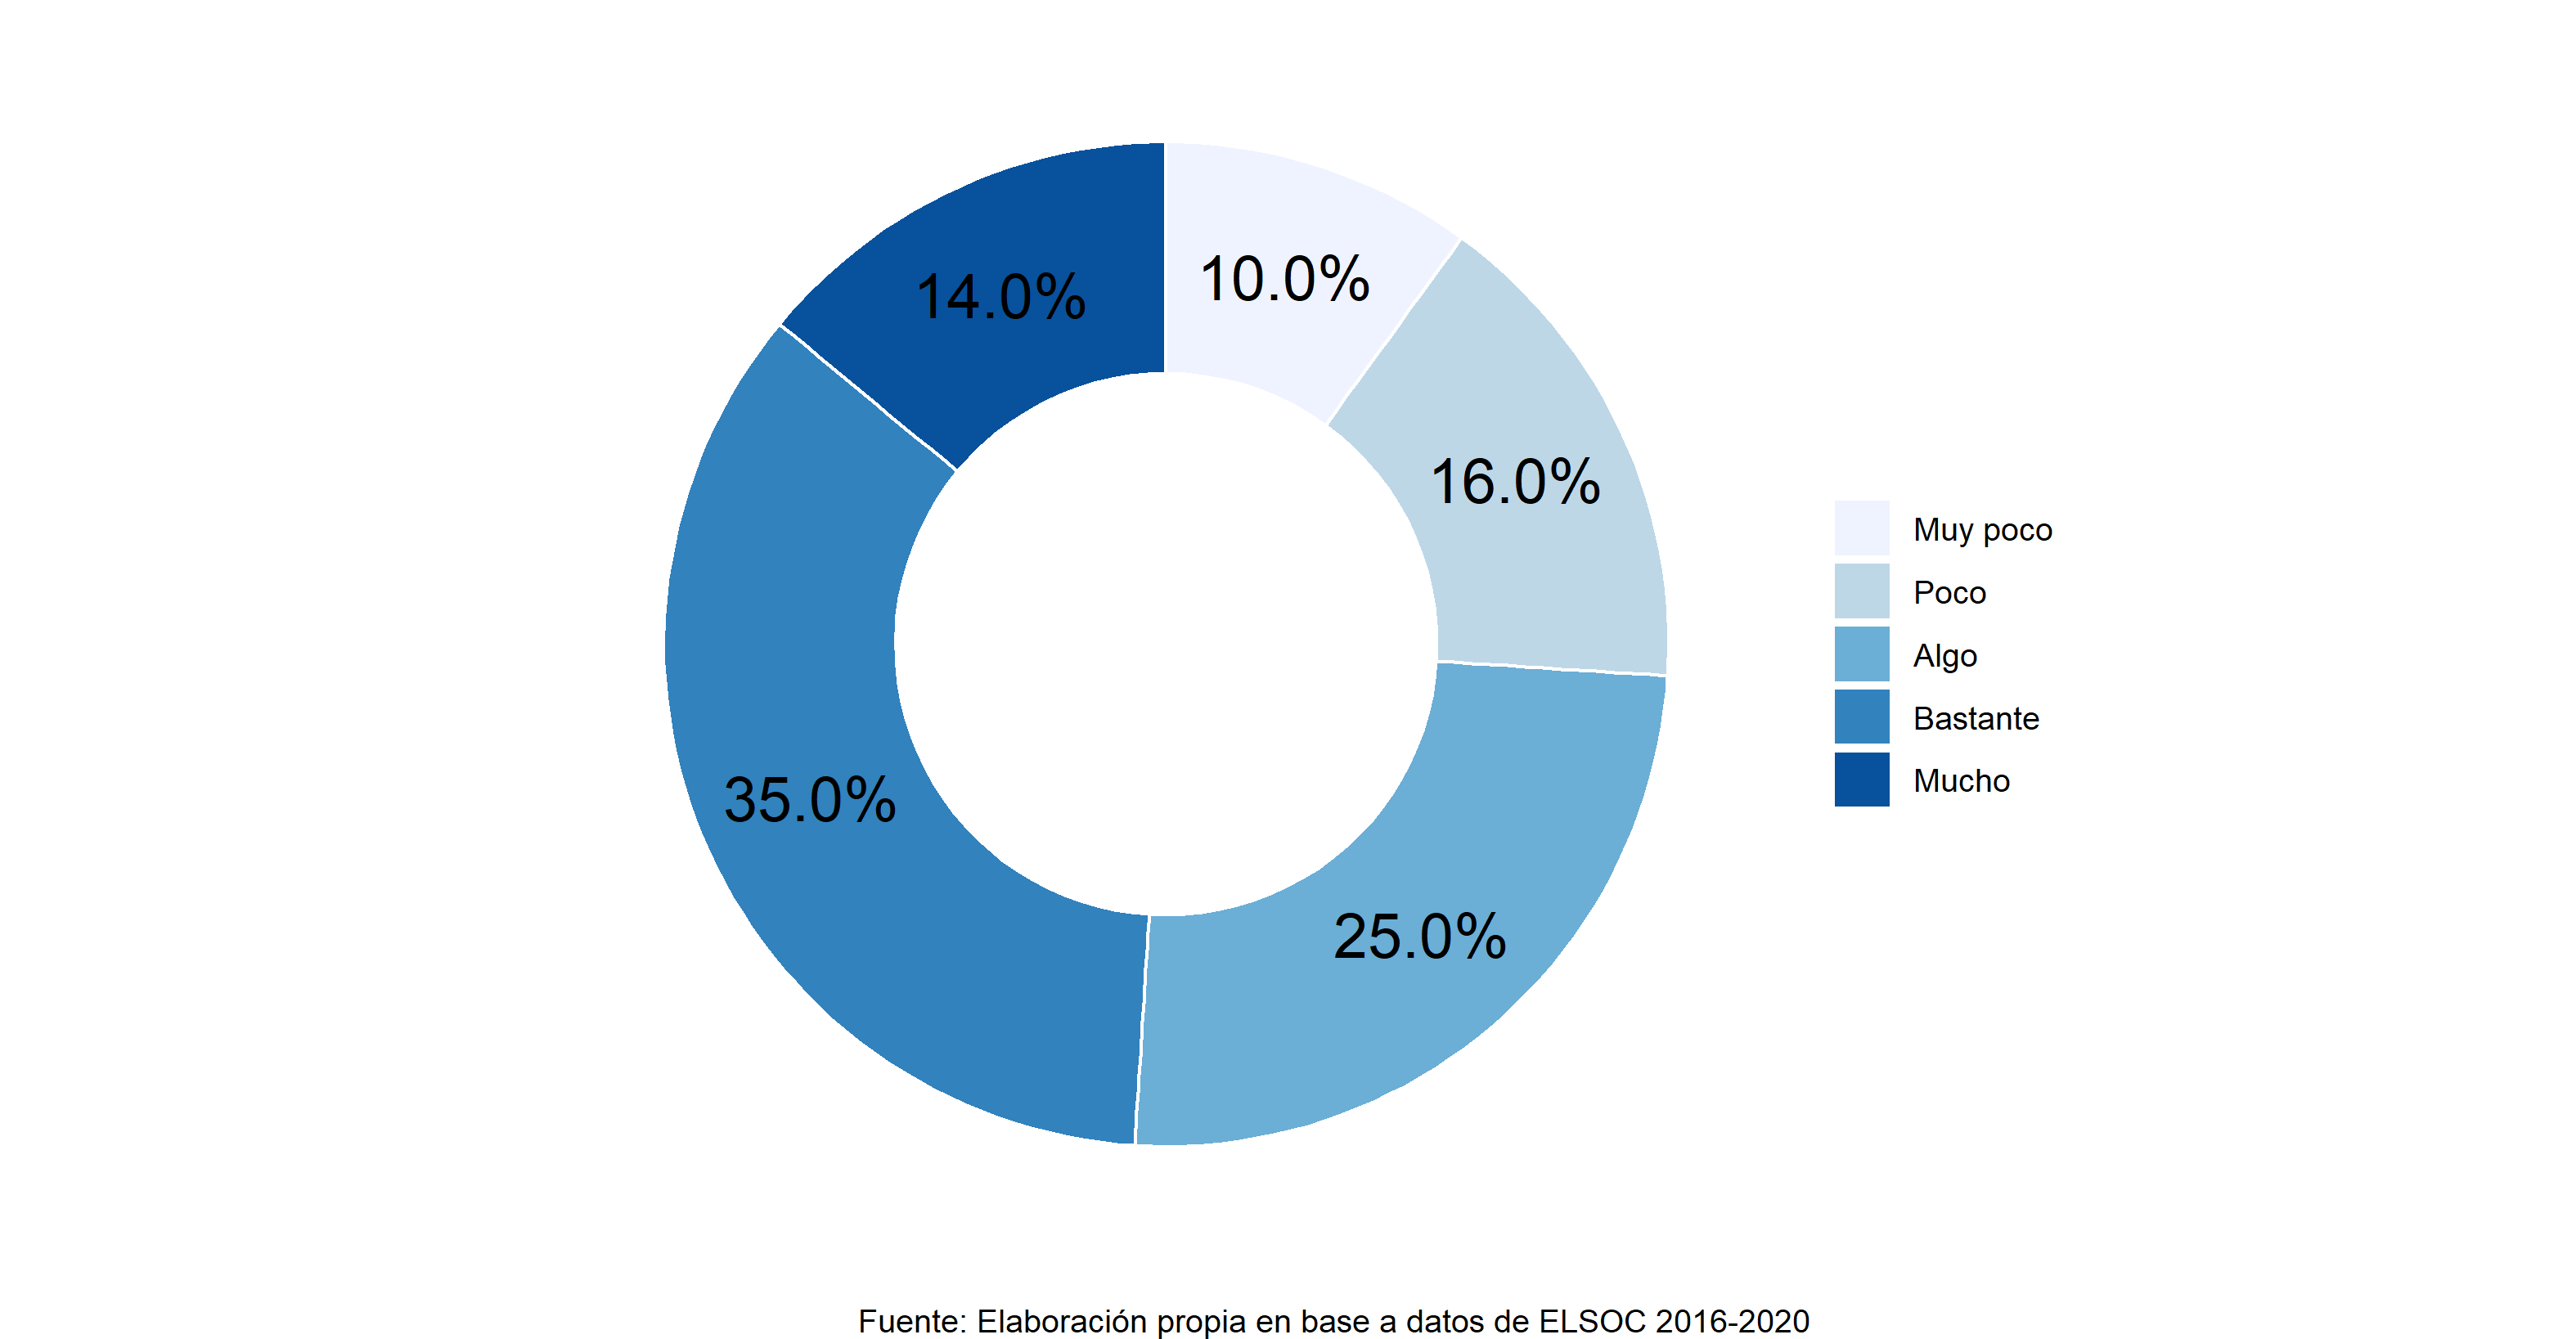
\includegraphics[width=1\linewidth,height=1\textheight]{output/graphs/confianza-vecinos} 

}

\caption{Confianza en vecinos.}\label{fig:confianza-vecinos}
\end{figure}

\textbf{Cohesión barrial}

Estos items abordan si las personas se sienten identificadas con la gente del barrio, si se sienten integrados, si se sienten parte del barrio y si creen que es su barrio ideal. Un gráfico descriptivo de estos cuatro items se presenta en la Figura \ref{fig:cohesion-barrial} y las correlaciones en la Figura \ref{fig:cohesion-barrial-cor}.

\begin{figure}[H]

{\centering 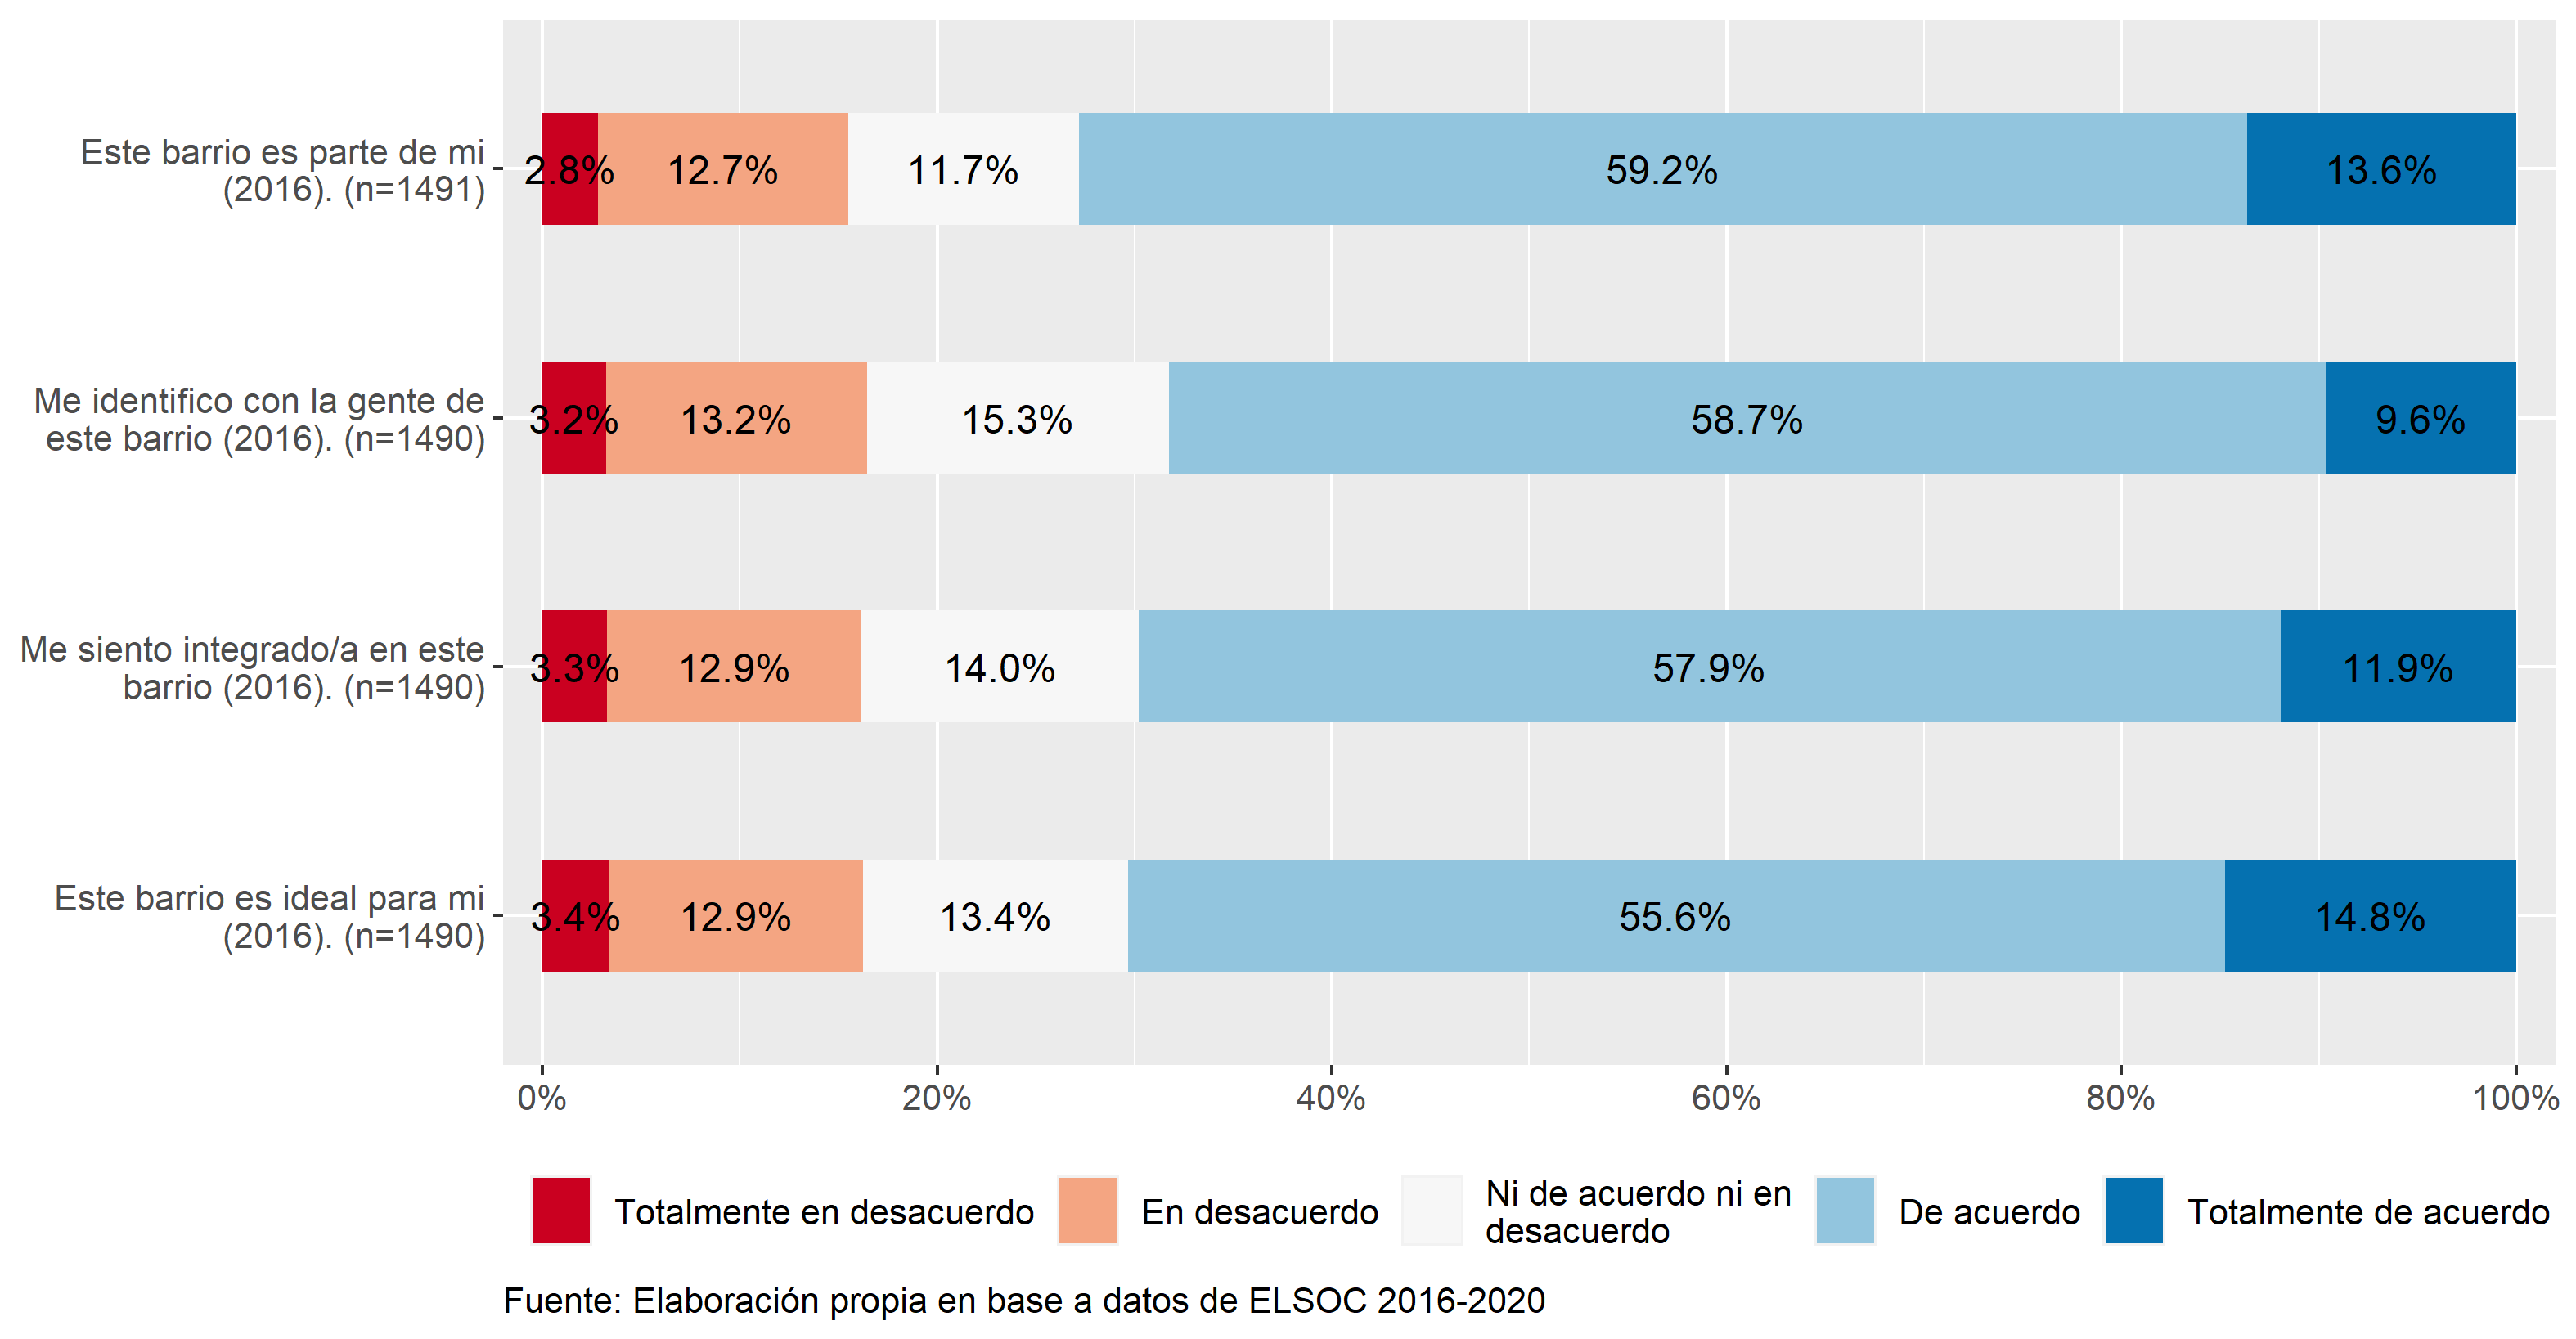
\includegraphics[width=1\linewidth,height=1\textheight]{output/graphs/cohesion-barrial} 

}

\caption{Cohesión en el barrio.}\label{fig:cohesion-barrial}
\end{figure}

\begin{figure}[H]

{\centering 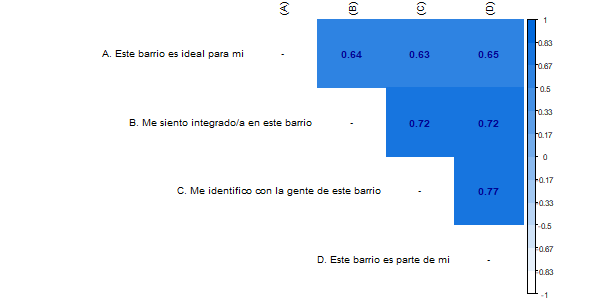
\includegraphics[width=1\linewidth,height=1\textheight]{output/graphs/cohesion-barrial_cor} 

}

\caption{Asociación indicadores cohesión barrial.}\label{fig:cohesion-barrial-cor}
\end{figure}

\textbf{Sociabilidad barrial}

Esta subdimensión de items territoriales presente en las cinco olas de ELSOC aborda la percepción sobre el barrio en relación con si las demás personas son sociables, si es fácil hacer amigos, si las personas son cordiales y si son colaboradoras. Un gráfico descriptivo de estos cuatro items se presenta en la Figura \ref{fig:sociabilidad-barrial} y un análisis bivariado en la Figura \ref{fig:sociabilidad-barrial-cor}.

\begin{figure}[H]

{\centering 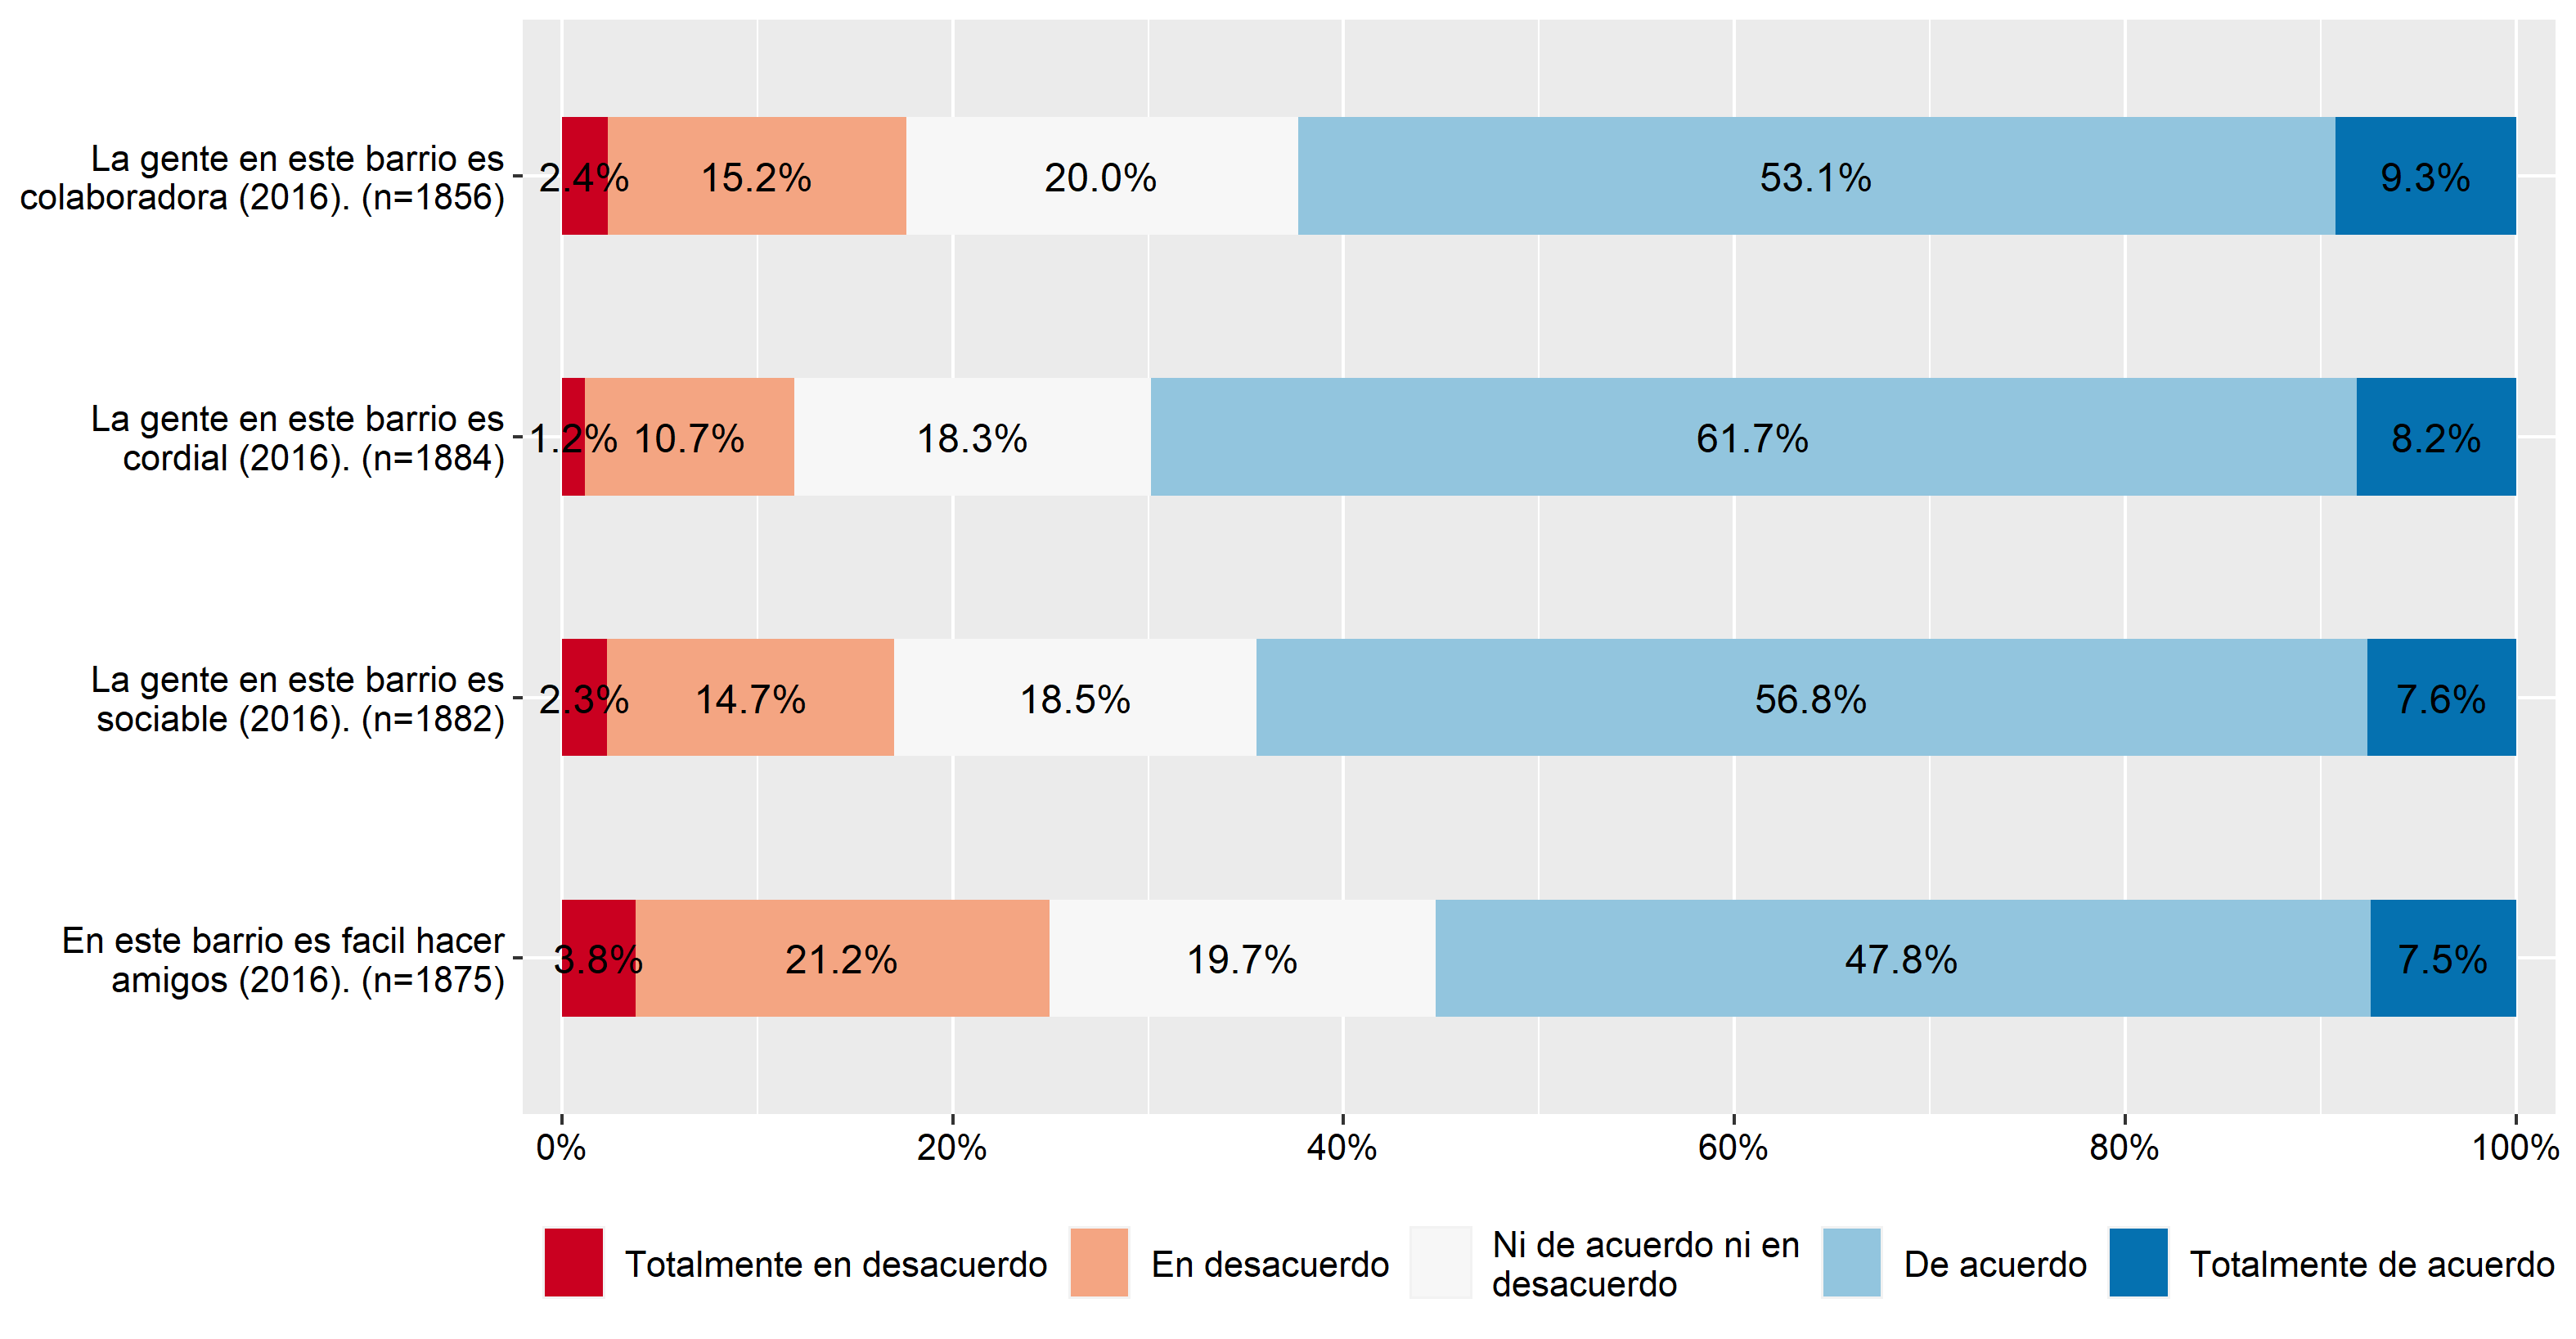
\includegraphics[width=1\linewidth,height=1\textheight]{output/graphs/sociabilidad-barrial} 

}

\caption{Sociabilidad barrial.}\label{fig:sociabilidad-barrial}
\end{figure}

\begin{figure}[H]

{\centering 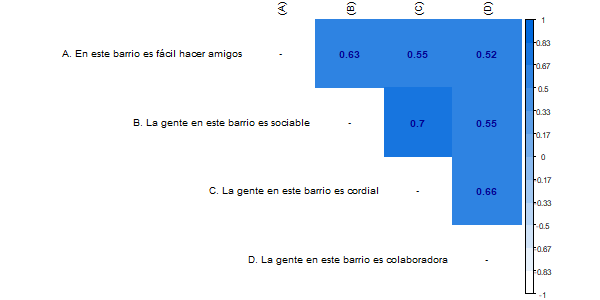
\includegraphics[width=1\linewidth,height=1\textheight]{output/graphs/sociabilidad-barrial_cor} 

}

\caption{Asociación indicadores sociabilidad barrial.}\label{fig:sociabilidad-barrial-cor}
\end{figure}

\textbf{Satisfacción residencial}

Finalmente, se incluye una subdimensión de Satisfacción Residencial, relacionada con items que miden la conectividad del barrio, la proximidad con el comercio, colegios, familiares y la principal actividad de trabajo, la limpieza del barrio, la cantidad de áreas verdes y la seguridad del barrio. Se incluye un gráfico descriptivo de estos ocho items en la Figura \ref{fig:satisfaccion-residencial} y un análisis bivariado en la Figura \ref{fig:satisfaccion-residencial-cor}.

\begin{figure}[H]

{\centering 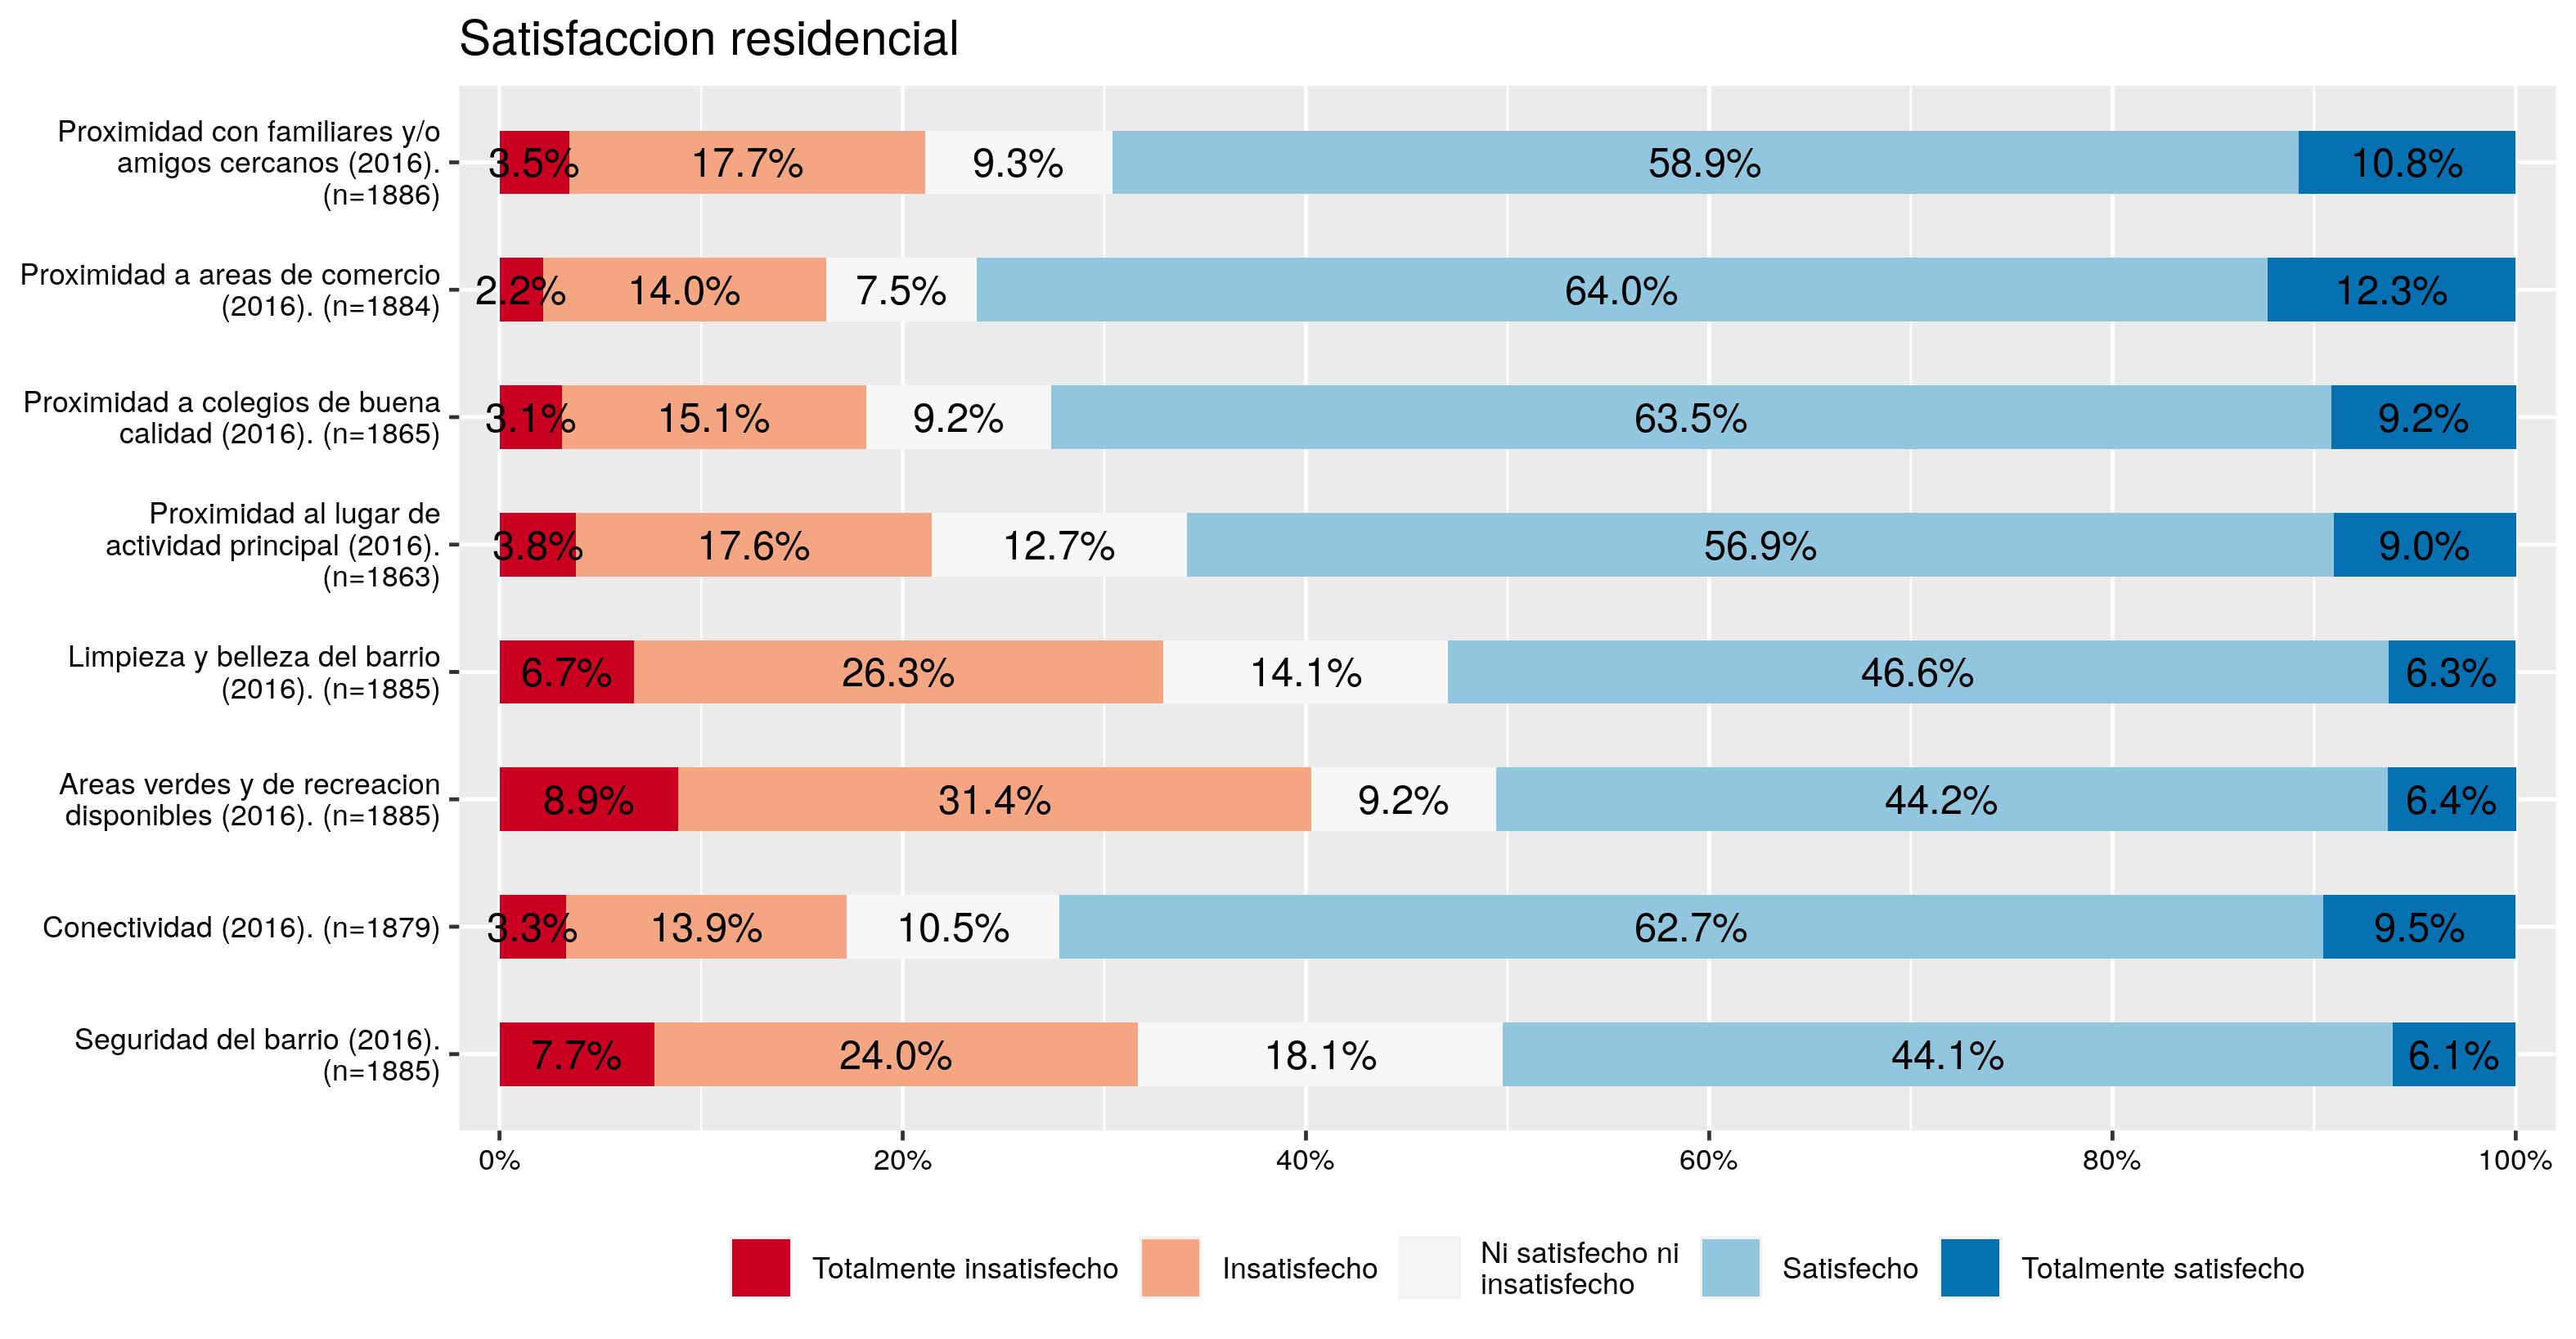
\includegraphics[width=1\linewidth,height=1\textheight]{output/graphs/satisfaccion-residencial} 

}

\caption{Satisfacción con el barrio.}\label{fig:satisfaccion-residencial}
\end{figure}

\begin{figure}[H]

{\centering 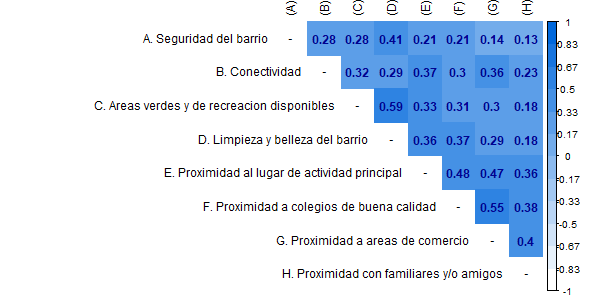
\includegraphics[width=1\linewidth,height=1\textheight]{output/graphs/satisfaccion-residencial_cor} 

}

\caption{Asociación indicadores satisfacción residencial.}\label{fig:satisfaccion-residencial-cor}
\end{figure}

Para la dimensión de cohesión territorial se realizó un único análisis factorial exploratorio. Como observamos en la Tabla \ref{tab:cohesion-territorial-fa}, en la segunda columna se presenta un factor que incluye los items referidos a la cohesión barrial, en la tercera columna se presenta un segundo factor asociado a la sociabilidad barrial y la confianza en vecinos y finalmente se presenta un tercer factor que incluye los items de satisfacción residencial. En cuanto a la varianza asociada a cada uno de estos factores, el primero de ellos representa el 15\% de la varianza, el segundo un 14\% de la varianza y el tercero un 13\% de la varianza. En base a estos resultados se propone utilizar un índice que incluya los cuatro items de cohesión barrial.

\begin{longtable}[]{@{}l@{}}
\caption{\label{tab:cohesion-territorial-fa}Dimensiones de cohesión territorial.}\tabularnewline
\toprule
\endhead

\includegraphics[width=8.33333in,height=\textheight]{output/tables/cohesion_territorial_fa.png} \\
\bottomrule
\end{longtable}

\hypertarget{relaciuxf3n-entre-las-subdimensiones-de-cohesiuxf3n-social}{%
\section{Relación entre las subdimensiones de cohesión social}\label{relaciuxf3n-entre-las-subdimensiones-de-cohesiuxf3n-social}}

Finalmente es relevante evaluar la consistencia del modelo teórico de cohesión social. En términos de medición esto se expresaría en que los indicadores que corresponden a una misma dimensión deberían correlacionar de manera moderada a alta entre sí, y de manera baja con las otras dimensiones. De ser así sería posible avanzar en la construcción de un indicador por dimensión, simplificando los análisis posteriores. De otra manera, en lo que sigue se debería analizar cada subdimensión por separado. Para poder evaluar este punto, la Figura \ref{fig:cohesion-social-cor} presenta información sobre la asociación entre las distintas subdimensiones de la cohesión social en base a los indicadores diseñados para cada una de ellas.

\begin{figure}[H]

{\centering 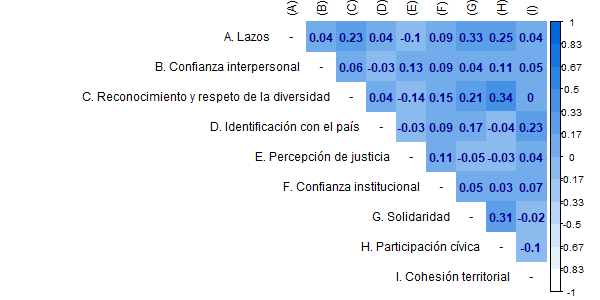
\includegraphics[width=1\linewidth,height=1\textheight]{output/graphs/cohesion_social_cor} 

}

\caption{Asociación de las subdimensiones de cohesión social.}\label{fig:cohesion-social-cor}
\end{figure}

Como se puede observar en la Figura \ref{fig:cohesion-social-cor}, las correlaciones entre las subdimensiones en general son bastante bajas, por lo tanto es difícil pensar en la construcción de indicadores de dimensiones a partir de sus respectivas subdimensiones. En este sentido, lo que se propone es el análisis de cada subdimensión por separado, manteniendo una coherencia conceptual desde dimensiones generales que provienen del modelo teórico de cohesión social de la CEPAL. De esta manera, en los capítulos que siguen se mantendrá la lógica de las dimensiones de cohesión social (relaciones sociales de igualdad, sentido de pertenencia, orientación hacia el bien común y la dimensión extra sobre territorio), pero analizando las subdimensiones por separado.

\hypertarget{cambios-en-la-cohesiuxf3n-social-en-chile-2016-2020}{%
\chapter{Cambios en la cohesión social en Chile 2016-2020}\label{cambios-en-la-cohesiuxf3n-social-en-chile-2016-2020}}

Este capítulo tiene como finalidad analizar la evolución de la opinión de las personas entre 2016 y 2020 respecto de las distintas dimensiones de la cohesión social presentadas en el capítulo 1. A través de este análisis longitudinal, se muestra no sólo la variación de la frecuencia de las respuestas en el tiempo, sino que además los cambios de opiniones de los respondentes entre olas. Estos cambios son representados con gráficos fluviales o aluviales. Recordamos que usamos las olas disponibles para cada dimensión de cohesión social construida en base a los indicadores detallados en el capítulo anterior.

El análisis presentado a continuación es de tipo descriptivo y de resumen, antes de pasar a la tercera parte del informe, que aborda los habilitadores e inhibidores de la cohesión social de manera más explicativa. Aquí no ahondamos en determinantes de la cohesión social, sino que presentamos información resumida en el tiempo para cerrar la primera parte del informe.

Adelantamos que en términos generales, existe poca varianza en los indicadores descritos a continuación en términos del tamaño de las categorías, pero pondremos el foco en quienes cambian de opinión de una ola a otra, que es uno de los aportes centrales del análisis longitudinal (que se representa en gráficos fluviales). La finalidad de esta sección es mostrar la evolución general en los últimos cinco años de las dimensiones constitutivas del sentido de pertenencia en Chile.

También señalamos que estos gráficos resumen una gran cantidad de información, la descrita en las secciones anteriores y la presenta gráficamente en una dimensión de tiempo, por lo que su meta es mostrar tendencias generales. Este tipo de gráfico es de uso reciente en Chile (ELSOC, 2020).

\hypertarget{relaciones-sociales-de-igualdad-1}{%
\section{Relaciones sociales de igualdad}\label{relaciones-sociales-de-igualdad-1}}

\hypertarget{confianza-interpersonal-grado-de-confianza-entre-personas}{%
\subsection{Confianza interpersonal (grado de confianza entre personas)}\label{confianza-interpersonal-grado-de-confianza-entre-personas}}

Los ítems que componen este indicador son dos:

\begin{itemize}
\item
  Se puede confiar en la mayoría de las personas
\item
  La mayoría de las personas tratan de ayudar a las demás
\end{itemize}

\begin{figure}[H]

{\centering 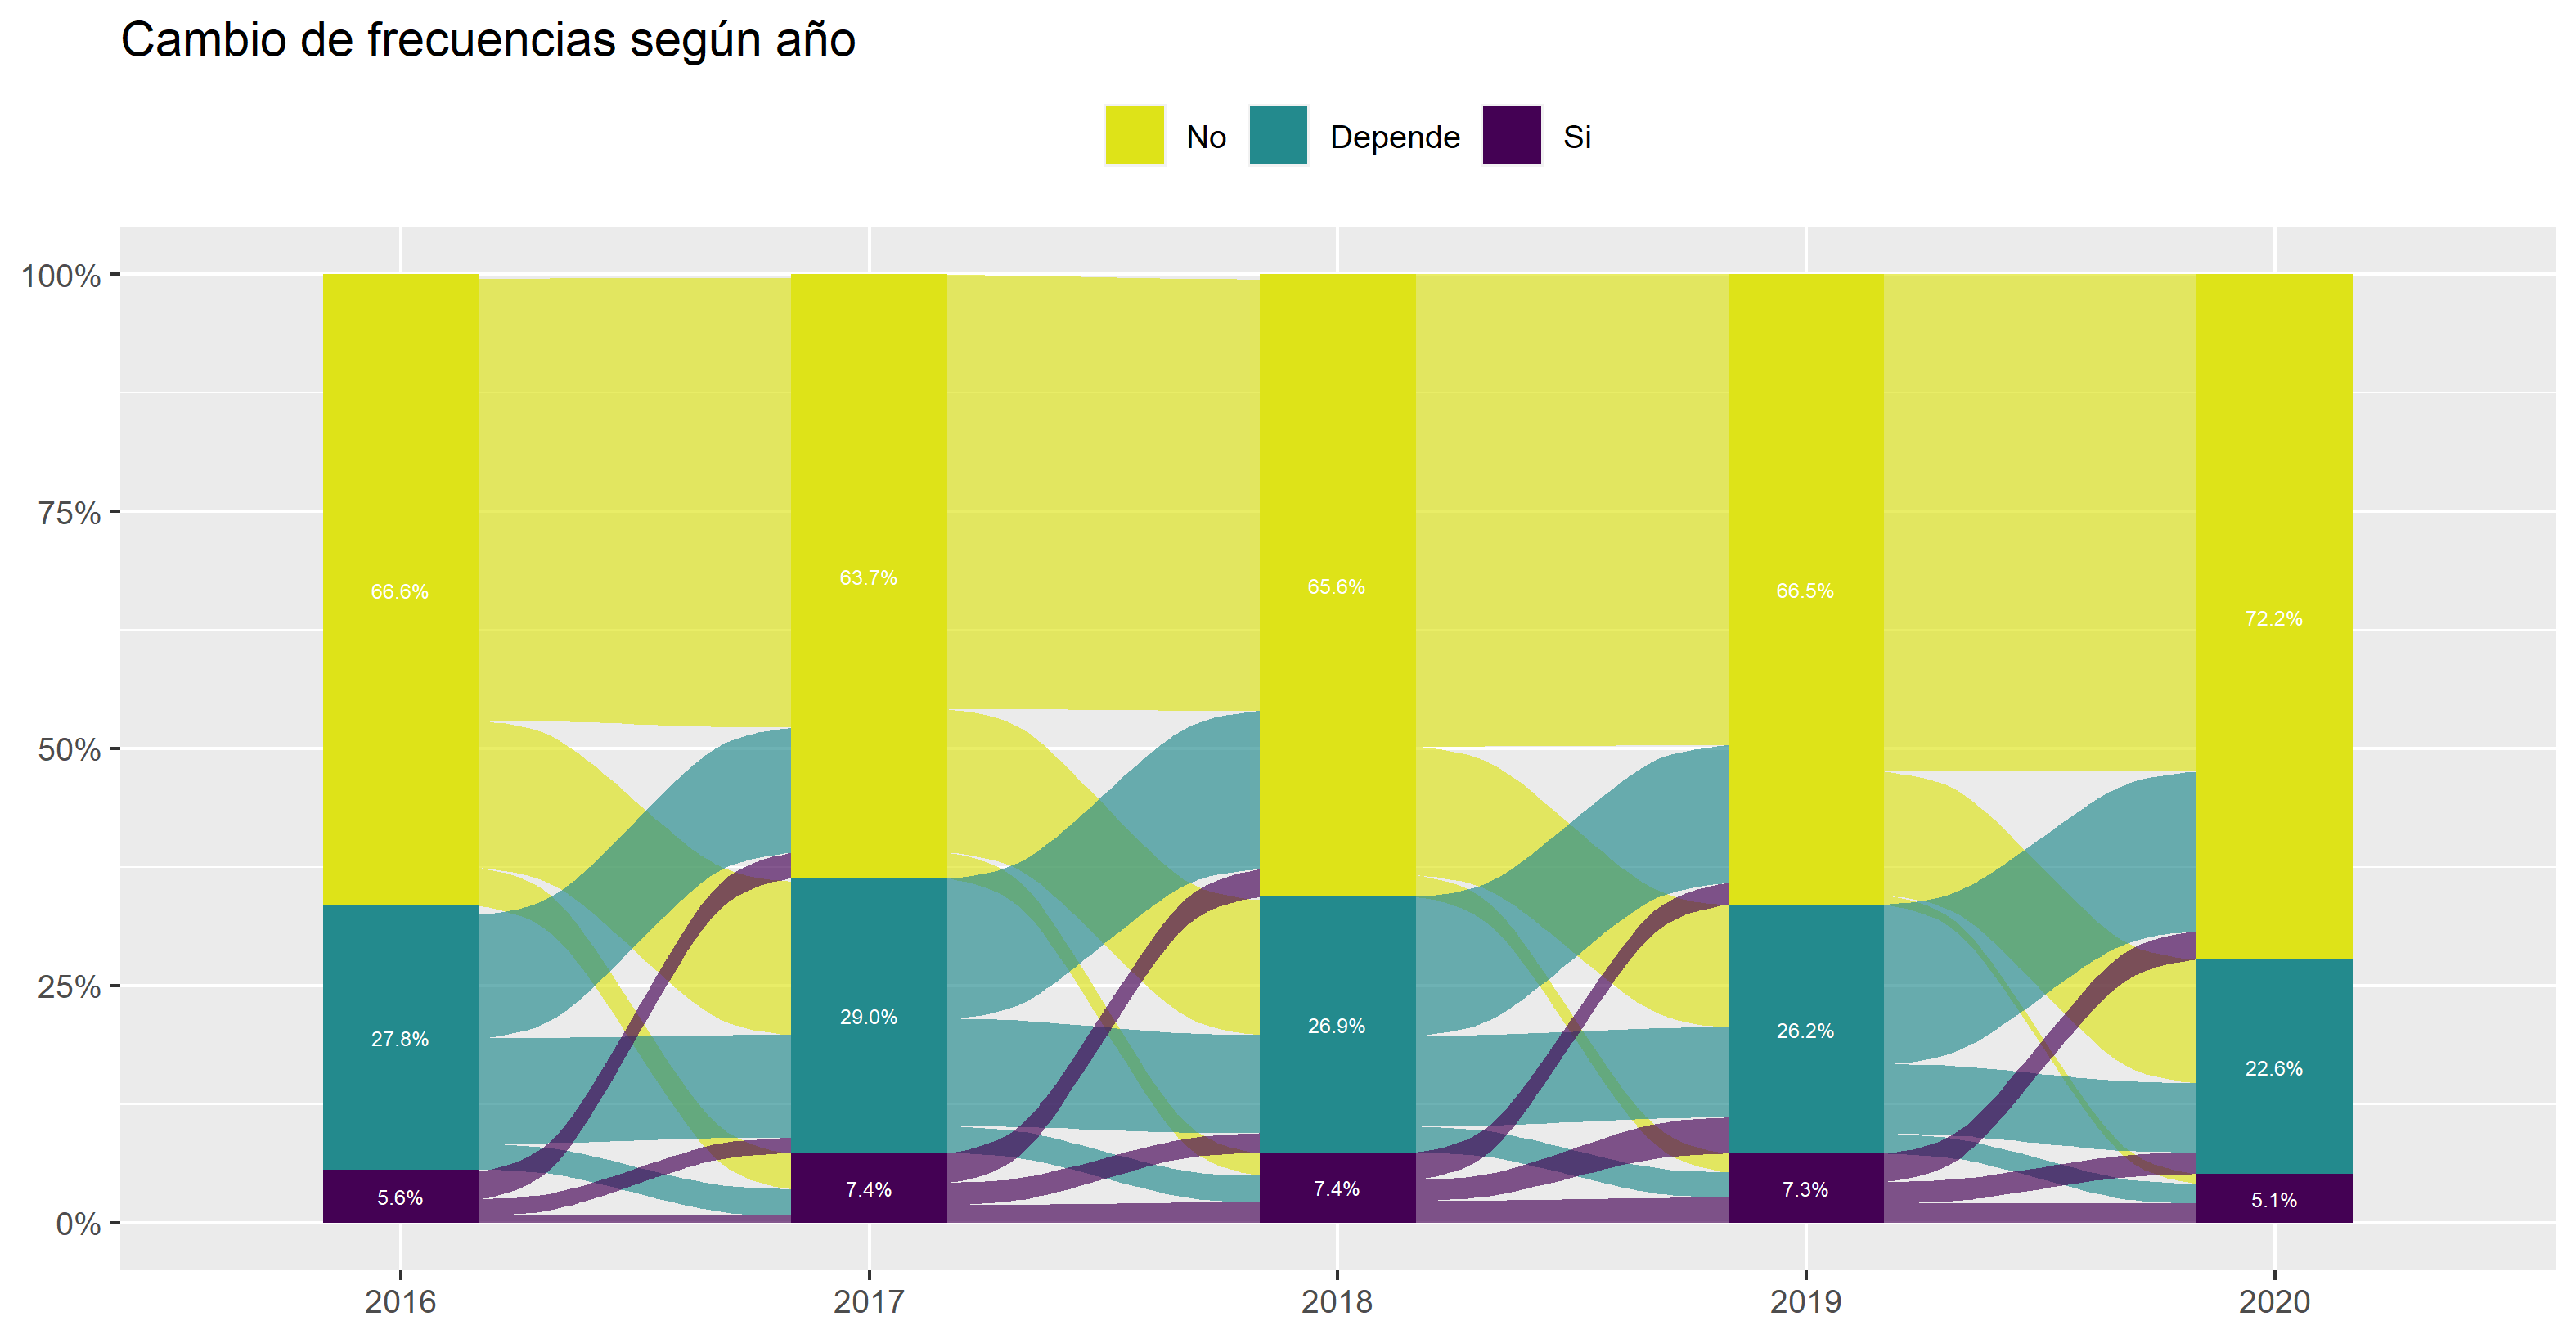
\includegraphics[width=1\linewidth,height=1\textheight]{output/graphs/alluvial_conf_interpersonal} 

}

\caption{Cambios en la subdimension confianza interpersonal.}\label{fig:alluvial-conf-interpersonal}
\end{figure}

En general, en la Figura \ref{fig:alluvial-conf-interpersonal} se observa una importante desconfianza hacia los demás en todas las olas, tal como era de esperarse en Chile, variando muy levemente entre un 66,6\% (2016) a un 72,2\% (2020). Las personas confiadas son absolutamente minoritarias, manteniéndose cerca de un 5\% en la primera y la última ola, con un leve aumento en las olas intermedias. Esta respuesta cambia poco en todo caso, manteniéndose alrededor de la cuarta parte de las respuestas para todas las olas, sin mayores variaciones.

En cuanto a las variaciones entre olas y entre respondentes, se observan algunos cambios de respuesta, aunque la mayor parte de quienes contestaron no mantiene su opinión a lo largo del período (alrededor del 50\% de los respondentes de la totalidad de la muestra). Los principales cambios son hacia la categoría ``depende''. Casi nadie cambia completamente de opinión en cuanto a confianza hacia las otras personas, salvo entre las olas 2016 y 2017, cuando el flujo es un poco más importante que en otros años. En cambio, respecto de las personas que señalan que ``depende'', en todos los años, se mantiene una mitad en la misma opción, mientras un grupo importante se cambia al grupo que expresa desconfianza hacia los demás en todos los años.

El estallido no alteró sustancialmente la percepción para el conjunto de la muestra en este elemento central de la cohesión social. La alta desconfianza interpersonal en Chile es una dimensión central de la cohesión social y no parece alterarse en el corto plazo, como se indica en este gráfico.

\begin{center}\rule{0.5\linewidth}{0.5pt}\end{center}

\emph{Recuadro metodológico: ¿Cómo leer un gráfico fluvial?}

Este tipo de diagrama muestra el cambio en el tiempo mediante flujos, usando una metáfora visual. Se trata de una representación esquemática y dinámica inspirada en el diagrama de Sankey, usado para dar cuenta de flujos energéticos. Su nombre proviene de los flujos - o clusters para fines de la lectura - que genera el agua y los diferentes arroyos contiguos que se forman de una misma fuente. Cada año funciona como un histograma apilado, donde la altura de cada barra indica el tamaño del cluster. Con la sucesión de los años, se observan los cambios en la composición de los clusters mediante los flujos. La amplitud de los flujos muestra el tamaño de los grupos de personas que cambian de opinión de un año a otro. Permiten a la vez ver la evolución de las categorías, así como los cambios y transiciones entre categorías y años. Los colores permiten visualizar las principales transiciones entre categorías (\protect\hyperlink{ref-rosvall_mapping_2010}{Rosvall \& Bergstrom, 2010}). Como no hay personas que salen de la muestra entre las cinco mediciones, no existen pérdidas en este gráfico.

\begin{center}\rule{0.5\linewidth}{0.5pt}\end{center}

\hypertarget{reconocimiento-y-respeto-de-la-diversidad}{%
\subsection{Reconocimiento y respeto de la diversidad}\label{reconocimiento-y-respeto-de-la-diversidad}}

Los ítems que componen este indicador son:

\begin{itemize}
\item
  Grado de confianza con personas homosexuales
\item
  Grado de confianza con personas mapuche
\item
  Grado de confianza con personas inmigrantes
\end{itemize}

\begin{figure}[H]

{\centering 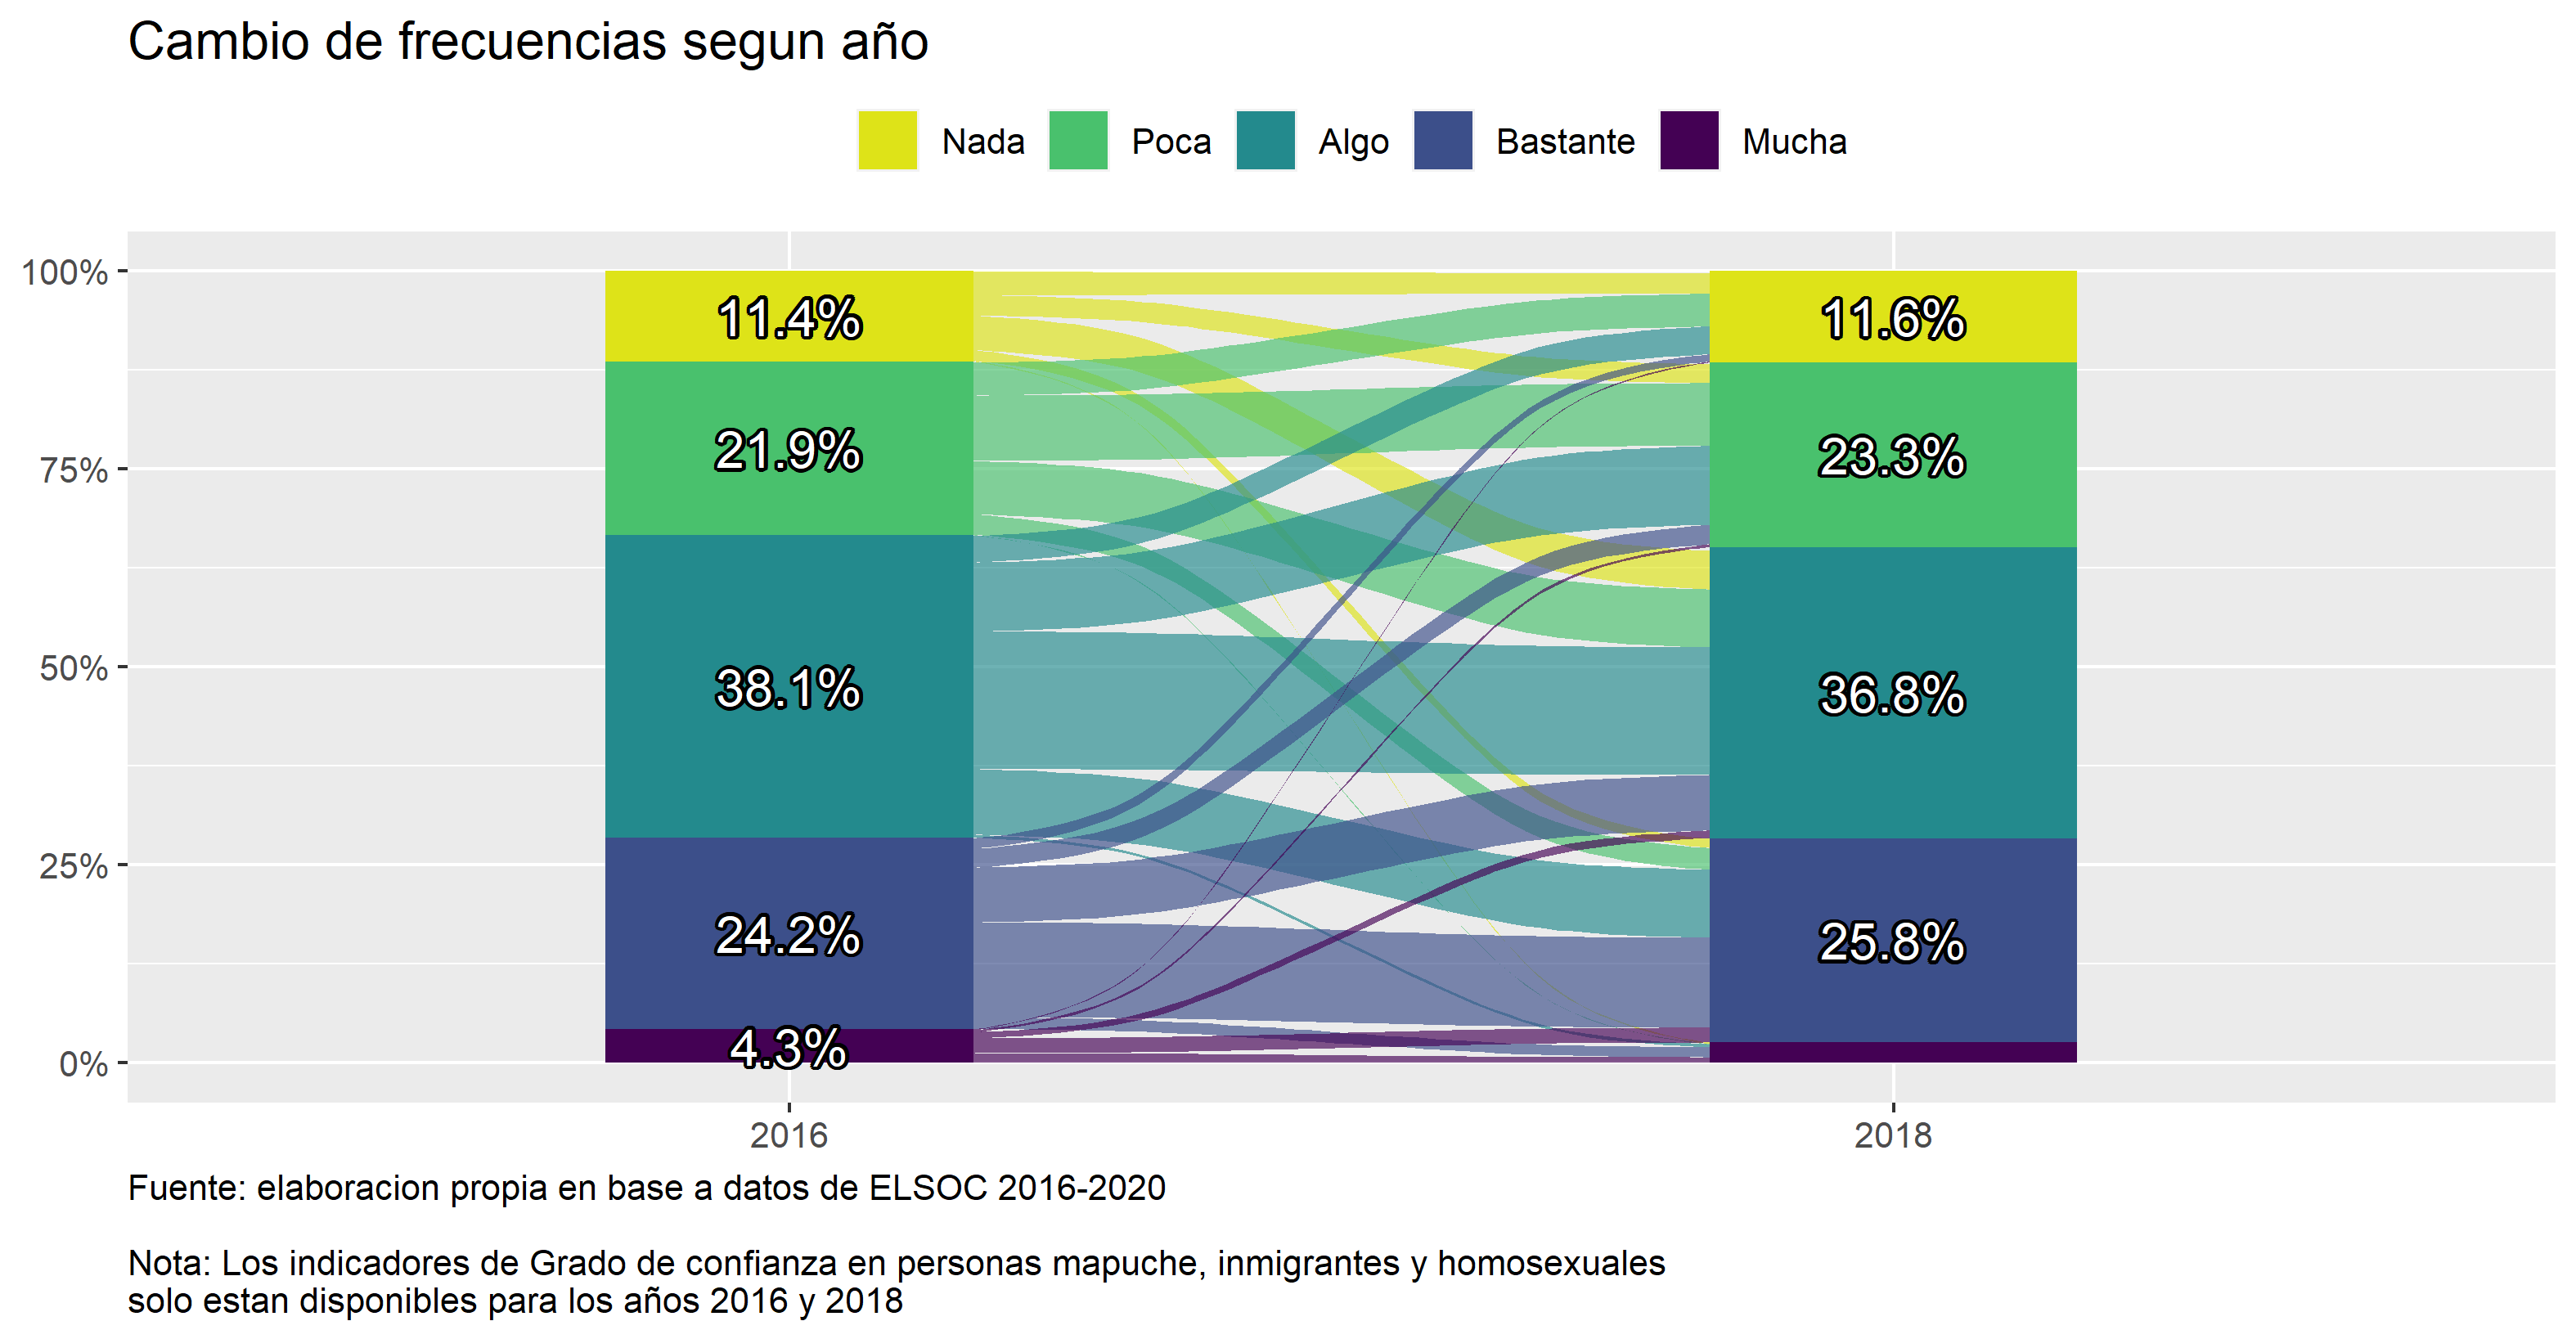
\includegraphics[width=1\linewidth,height=1\textheight]{output/graphs/alluvial_diversidad} 

}

\caption{Cambios en la subdimension reconocimiento y respeto de la diversidad.}\label{fig:alluvial-diversidad}
\end{figure}

Contamos solo con dos olas ya que estos ítems no se incluyen en la ola 2020 de ELSOC, por lo que es poco interpretable en términos longitudinales. De todas formas se realiza el ejercicio de análisis.

En general, en la Figura \ref{fig:alluvial-diversidad} las respuestas son muy estables en frecuencia entre las dos olas para el reconocimiento y el respeto de la diversidad. La categoría más numerosa es la intermedia, es decir ``algo'', del 38\% de las respuestas, es decir con un grado moderado de confianza hacia personas que la sociedad asume como diferentes. Si sumamos ``nada'' y ``poca'' confianza hacia personas diversas, por un lado, se suma alrededor del 33\% de las respuestas en ambas olas, mientras al añadir las respuestas ``bastante'' y ``mucha'', la frecuencia es un poco mayor a las respuestas desconfiadas hacia la diversidad, alrededor del 27\%. Observamos por lo tanto casi tres tercios equilibrados y constantes al agrupar las respuestas.

En cuanto a las variaciones entre olas y entre respondentes, en general las opiniones se mantienen de forma mayoritaria, salvo para la categoría ``nada'\,', que tiende a repartirse en todas las demás categorías, salvo la máxima (``mucha''). El grupo más estable entre las dos olas corresponde a las personas que expresan ``algo'' de confianza hacia las personas diversas. Las personas que expresan confianza y respeto hacia la diversidad en la ola 2016 (con las categorías ``bastante'' o ``mucha'') pueden cambiarse a la categoría inferior, pero no al otro extremo.

\hypertarget{lazos-cantidad-de-personas-que-se-conocen-con-diferentes-ocupaciones}{%
\subsection{Lazos (cantidad de personas que se conocen con diferentes ocupaciones)}\label{lazos-cantidad-de-personas-que-se-conocen-con-diferentes-ocupaciones}}

Este indicador se compone del item ``Cantidad de personas que se conocen con diferentes ocupaciones''

\begin{figure}[H]

{\centering 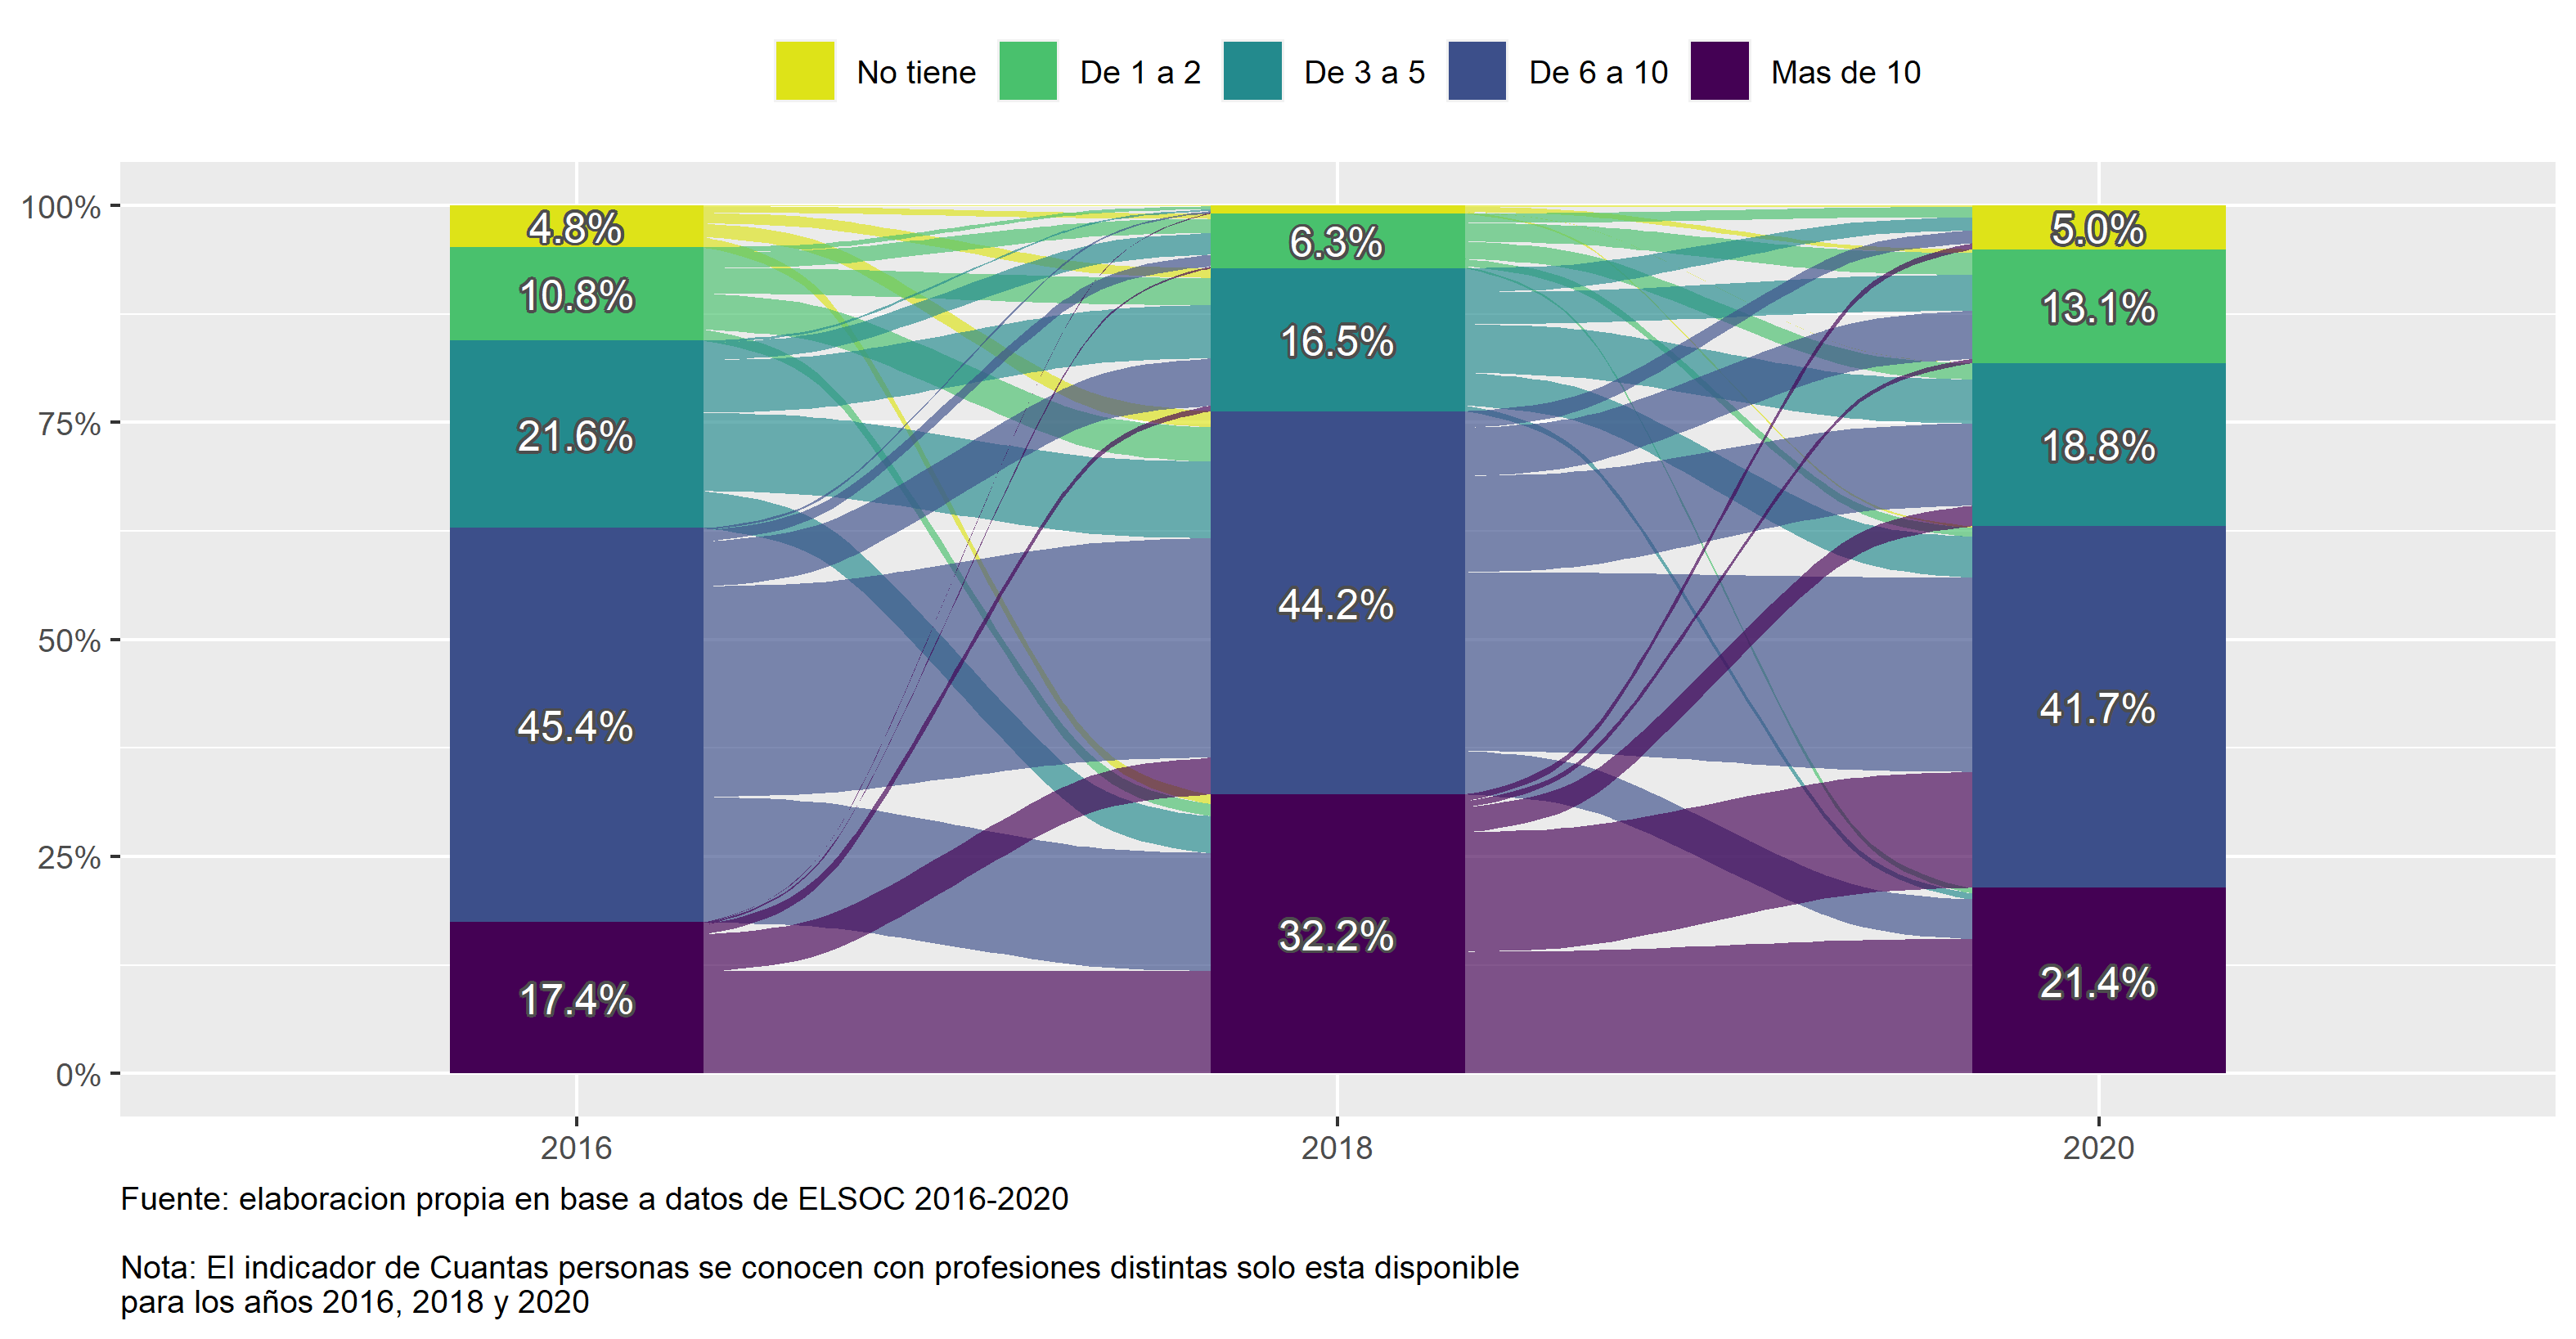
\includegraphics[width=1\linewidth,height=1\textheight]{output/graphs/alluvial_lazos} 

}

\caption{Cambios en la subdimensión Lazos.}\label{fig:alluvial-lazos}
\end{figure}

En general, en la Figura \ref{fig:alluvial-lazos} se observa una importante estabilidad entre los años 2016 y 2020 respecto al número de personas que los respondentes declaran conocer con diferentes ocupaciones, aunque existen variaciones no menores para el año 2018, que no son fáciles de interpretar. Las categorías de más contactos (de 6 a 10 y más de 10) concentran una mayoría de respuestas para los años 2016 y 2020 (alrededor del 62\%). Las categorías con menos contactos con diferentes ocupaciones (1 a 2 y 3 a 5) alcanzan un 31\% para los años 2016 y 2020, mientras la categoría con menos frecuencia corresponde a las personas que no declaran contactos en diferentes ocupaciones en ninguna de las tres olas (menos del 5\%).

En cuanto a las variaciones entre olas y entre respondentes, las frecuencias varían significativamente de una ola a otra, salvo para las categorías con mayores contactos en diferentes ocupaciones, que mayoritariamente se mantienen (de 6 a 10 y más de 10). Los cambios más importantes, dentro de la minoría que cambia de respuesta, se da hacia categorías colindantes, sin cambios entre categorías extremas.

En resumen, el número de personas que los respondentes declaran conocer con diferentes ocupaciones es un indicador relativamente estable de cohesión social para el período completo, pero con importantes cambios de respuesta entre las mismas personas de una ola a otra.

\hypertarget{sentido-de-pertenencia-1}{%
\section{Sentido de pertenencia}\label{sentido-de-pertenencia-1}}

\hypertarget{identificaciuxf3n-con-el-pauxeds}{%
\subsection{Identificación con el país}\label{identificaciuxf3n-con-el-pauxeds}}

Los ítems que componen este indicador son

\begin{itemize}
\item
  Me siento orgulloso de ser chileno
\item
  Me identifico con Chile
\end{itemize}

\begin{figure}[H]

{\centering 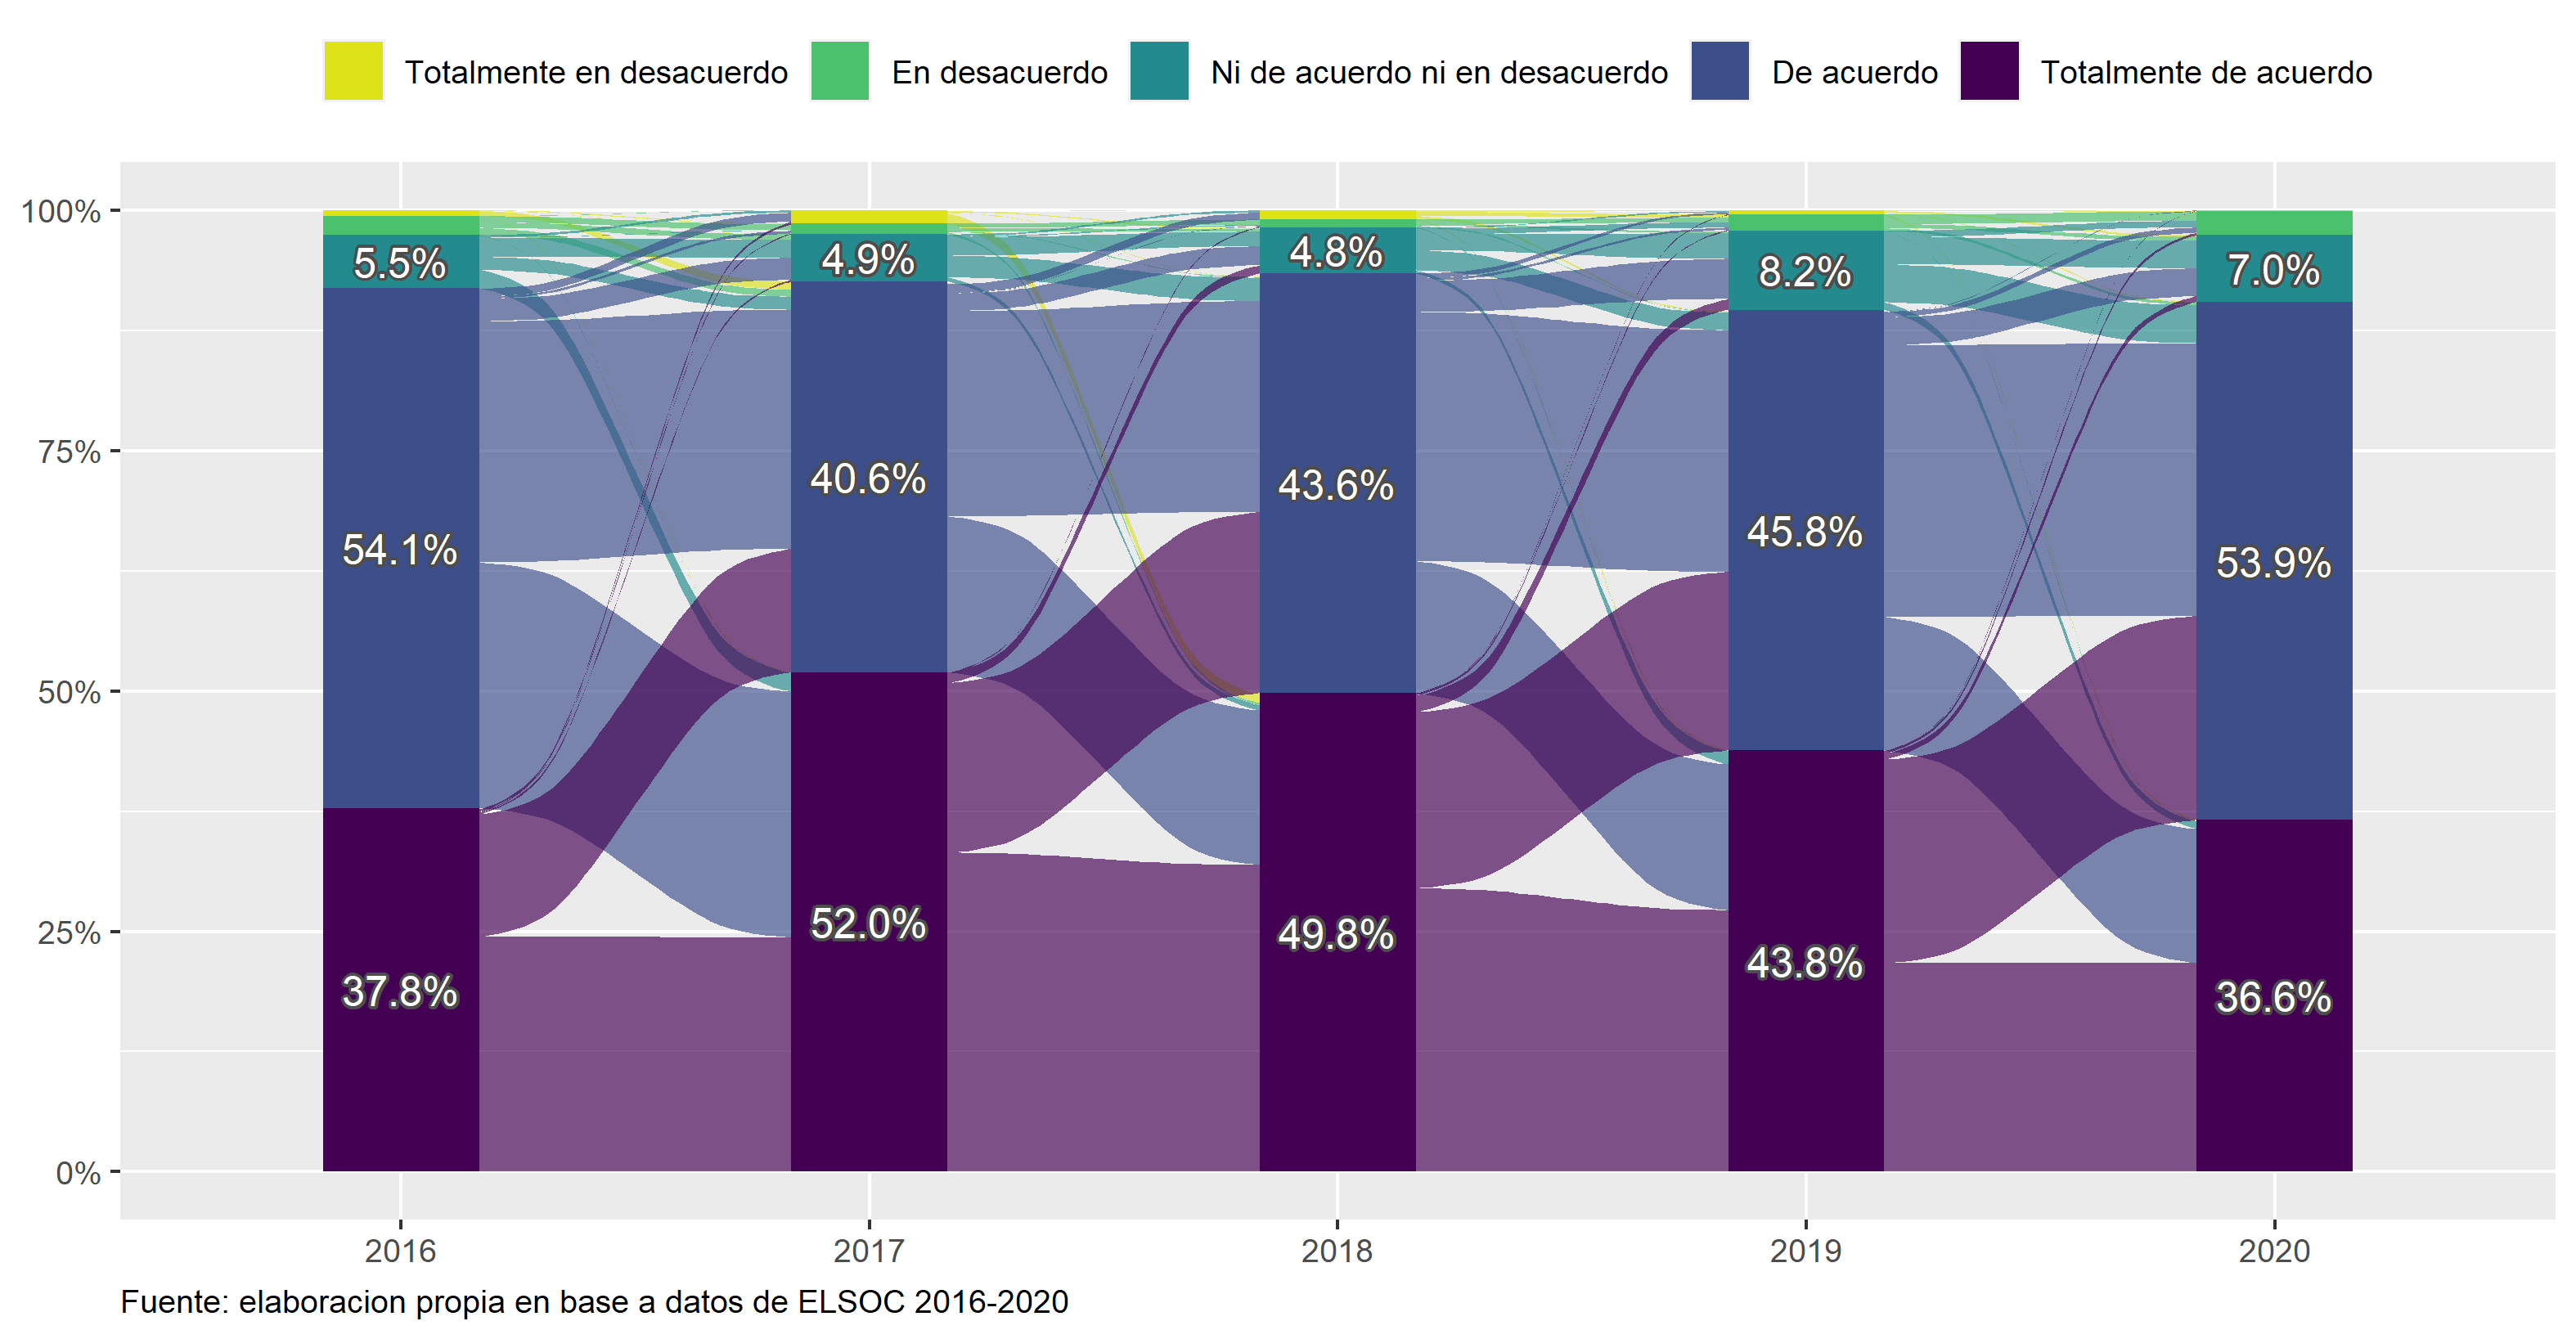
\includegraphics[width=1\linewidth,height=1\textheight]{output/graphs/alluvial_identificacion} 

}

\caption{Cambios en la subdimensión identificacion con el pais.}\label{fig:alluvial-identificacion}
\end{figure}

En general, en cuanto a la identificación con Chile o el orgullo de ser chileno de la Figura \ref{fig:alluvial-identificacion}, para las cinco olas, la cantidad de personas que no se identifican con Chile es mínima (correspondiente a las categorías ``totalmente en desacuerdo'' y ``en desacuerdo''). La categoría intermedia (``ni en desacuerdo ni de acuerdo'') no varía tampoco entre olas y es muy baja (entre el 5\% y el 8\%). Las respuestas ``de acuerdo'' y ``muy de acuerdo'', que indican una identificación fuerte o muy fuerte con Chile recogen una cantidad abrumadora de respuestas, sumando más del 90\% de las opciones en todas las olas. Esto indica una identificación elevada y constante, aunque existen variaciones entre la categoría ``muy de acuerdo'', que indica una identificación muy fuerte y la categoría ``de acuerdo'' entre las distintas olas. Llama la atención la baja de la categoría ``totalmente de acuerdo'' en las tres últimas olas, pasando de un 52\% a un 36.6\%, una de las variaciones más notables en los gráficos analizados en este capítulo, incluida una caída fuerte en 2019-2020.

En cuanto a las variaciones entre olas y entre respondentes, se da sobre todo entre las categorías de mayor identificación con Chile, en proporciones que varían del tercio a la mitad de los respondentes. La categoría más estable en el tiempo es ``ni de acuerdo ni en desacuerdo''. Existe un leve flujo entre la categoría ``ni en desacuerdo ni de acuerdo'' y ``en desacuerdo'', pero es bastante menor, aunque un poco más elevada entre el 2018 y el 2019, flujo que se revierte al año siguiente.

Nuevamente estamos frente a categorías con poca varianza y la identificación con Chile es estable en el tiempo si se miran solo 3 categorías, pero con una interesante baja de la identificación más fuerte en las tres últimas olas hasta un menos comprometido ``de acuerdo''.

En resumen, el estallido del 2019 no alteró sustancialmente la percepción para el conjunto de la muestra en términos binarios (respecto de si las personas se identifican o no con Chile) pero sí es notoria la pérdida de 15 puntos de la categoría de identificación más fuerte hacia una identificación menos intensa en los tres últimos años, particularmente entre las dos últimas olas.

\hypertarget{percepciuxf3n-de-justicia}{%
\subsection{Percepción de justicia}\label{percepciuxf3n-de-justicia}}

Los ítems que componen este indicador son

\begin{itemize}
\item
  En Chile las personas son recompensadas por sus esfuerzos
\item
  En Chile las personas son recompensadas por su inteligencia
\end{itemize}

\begin{figure}[H]

{\centering 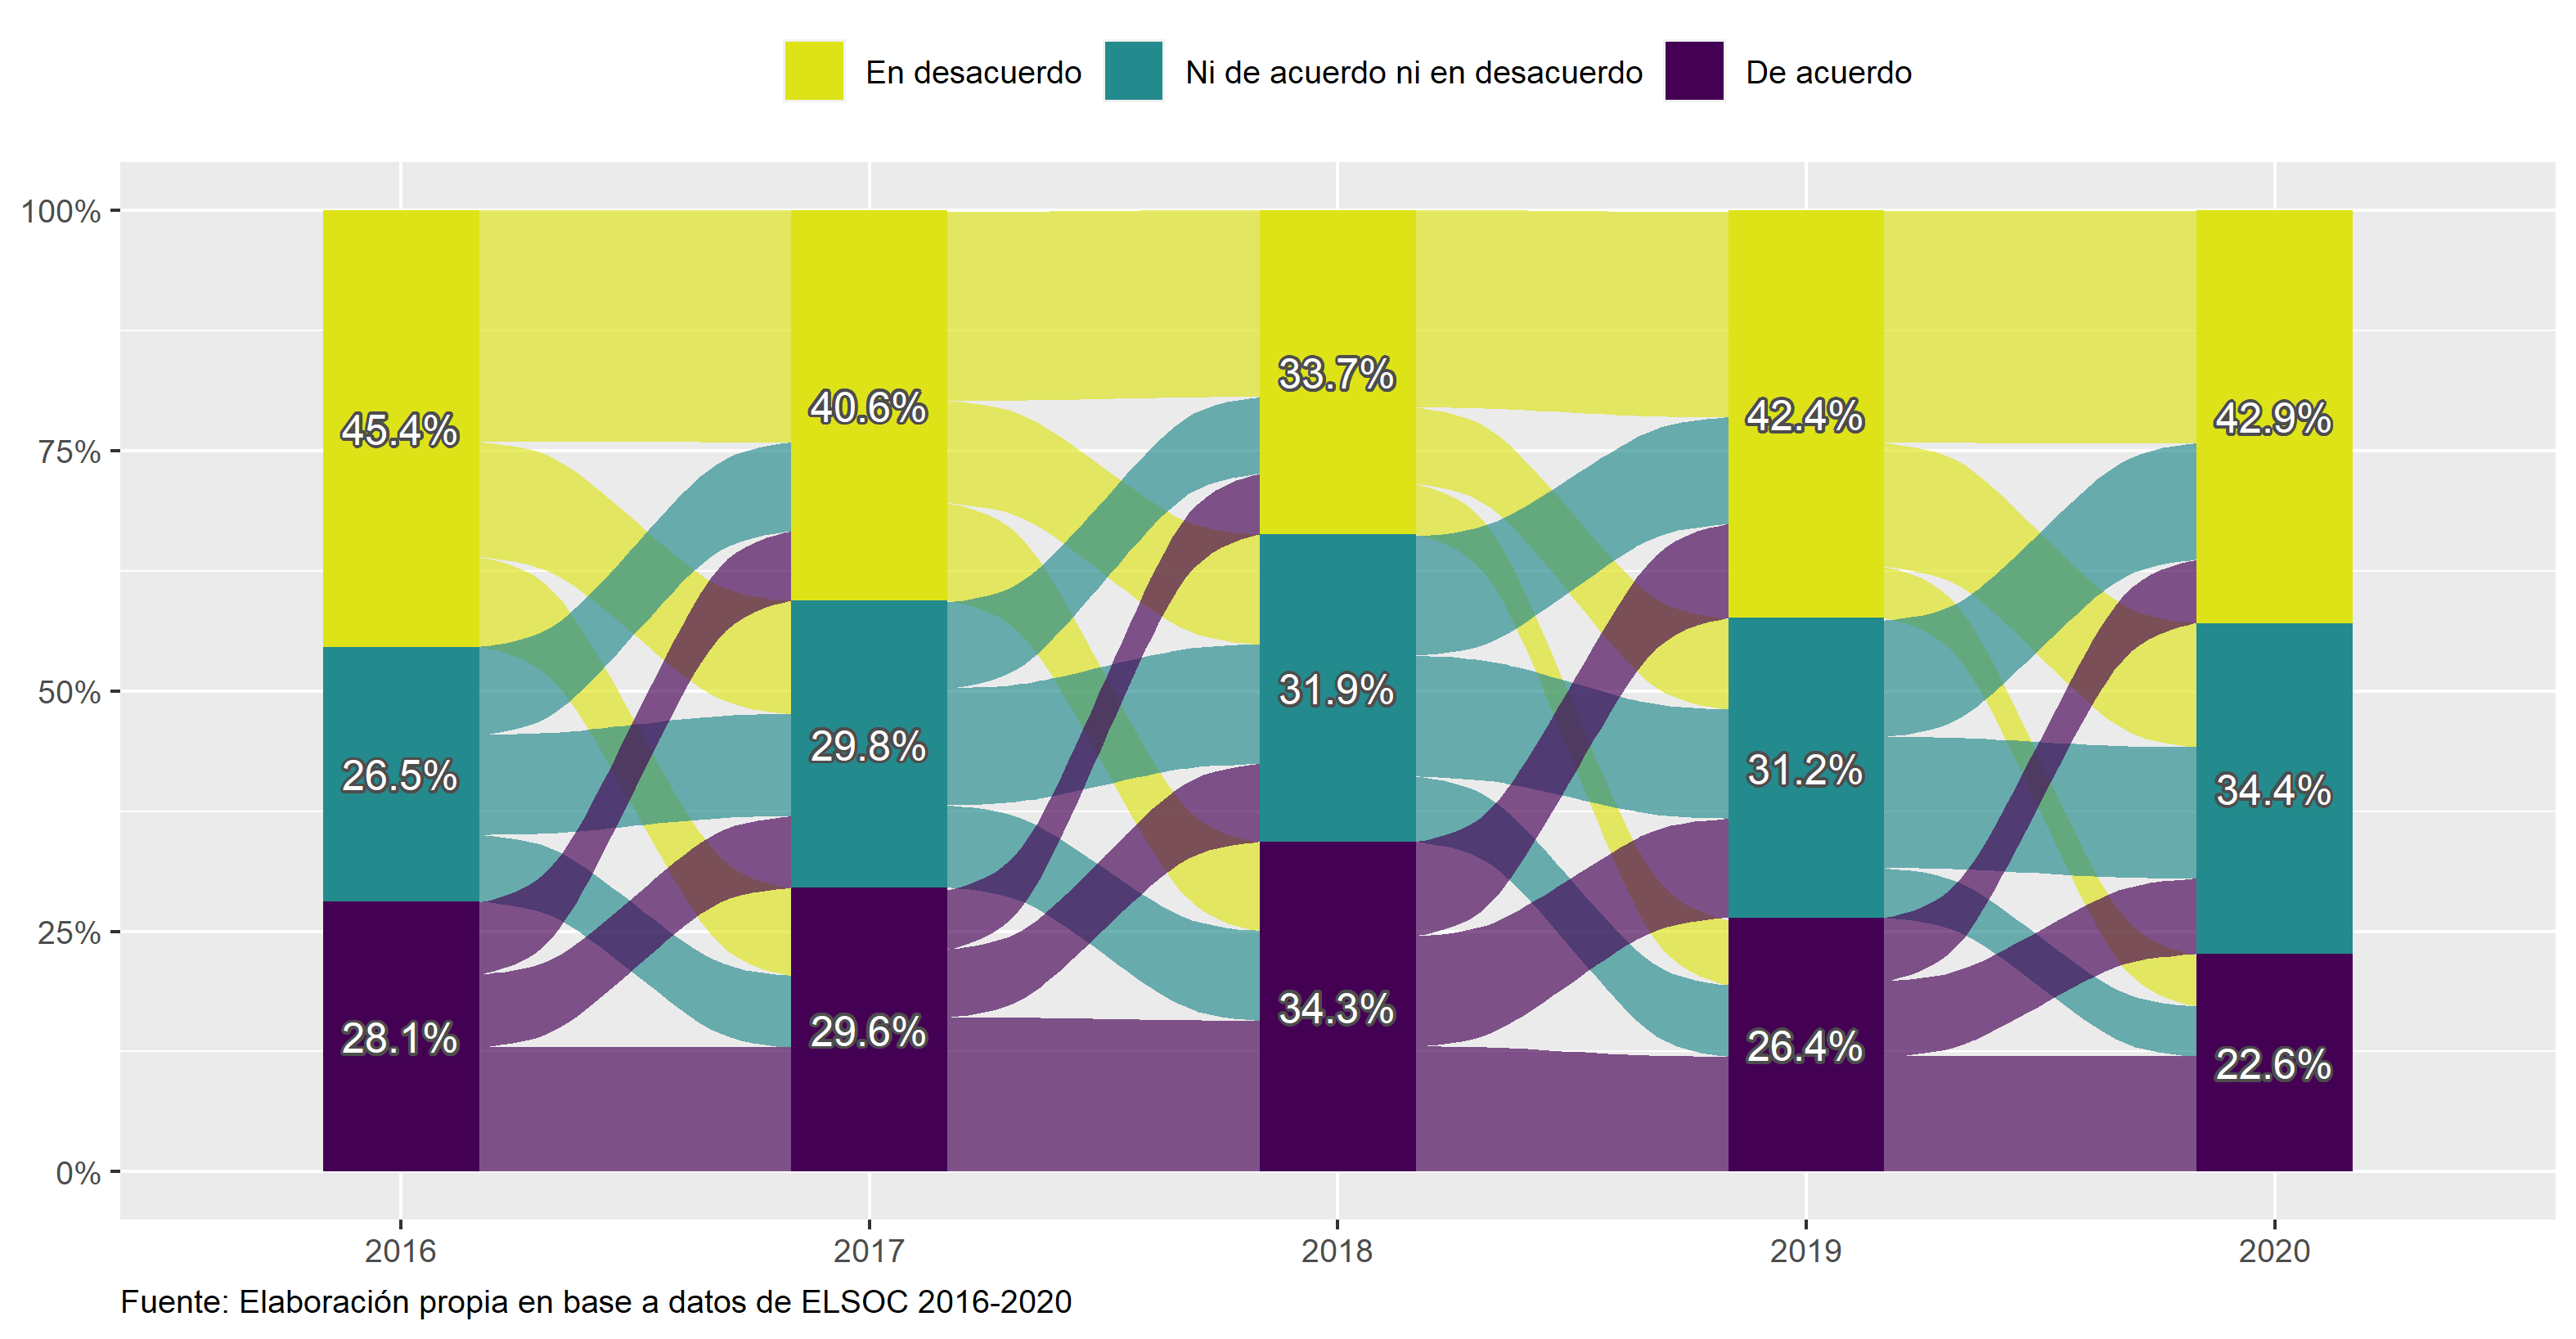
\includegraphics[width=1\linewidth,height=1\textheight]{output/graphs/alluvial_justicia} 

}

\caption{Cambios en la subdimensión percepcion de justicia.}\label{fig:alluvial-justicia}
\end{figure}

En general, respecto de si la inteligencia y el esfuerzo son recompensados en Chile, datos que se observa en la Figura \ref{fig:alluvial-justicia}, existen pocas variaciones entre olas. La más abultada es ``En desacuerdo'', con una frecuencia promedio del 41\%, seguida por ``Ni de acuerdo ni en desacuerdo (alrededor del 30\%) y finalmente viene la opción ``De acuerdo'' con alrededor del 28\% de las preferencias en promedio. Esto indica que en general los respondentes consideran más bien que no se recompensa la inteligencia ni el esfuerzo en Chile. Sin embargo, cabe notar que entre 2016 y 2018, la cantidad de personas que están en desacuerdo con la idea de que en Chile se recompensan los esfuerzos y la inteligencia baja de casi 12 puntos, lo que es una evolución notoria. Este juicio vuelve a tener más importancia en las olas 2019 y 2020, llegando a un nivel estable en ambos años del 42\%. Esta evolución se nota también en la categoría ``De acuerdo'', que fluctúa como espejo respecto de ``En desacuerdo''. Aunque recoge menos opciones que la categoría con el juicio negativo, aumenta en 6 puntos entre 2016 y 2019 antes de volver a bajar, con una pérdida importante de 12 puntos entre 2018 y 2020, lo que se podría corresponder con percepciones ampliamente vehiculizadas por el estallido social de 2019.

En cuanto a las variaciones entre olas y entre respondentes, la mitad de los respondentes mantiene su opción entre olas, salvo para la opción ``Ni de acuerdo ni en desacuerdo''. No son entonces categorías particularmente estables en el tiempo. Si bien las variaciones más importantes se dan entre categorías colindantes, existen flujos no menores entre categorías extremas que indican que alrededor del 5 a 8\% de los respondentes puede haber sufrido un cambio importante en su percepción.

En resumen, el estallido del 2019 no alteró sustancialmente la percepción para el conjunto de la muestra, lo que llama la atención, porque pudo ser una variable más determinada por el contexto y en especial por la mayor evidencia de la desigualdad y la injusticia en Chile que la anterior por ejemplo (identificación con el país). Sin embargo, se observa una importante volatilidad de un año a otros, por lo que este indicador es uno de los menos estables en el tiempo en relación con los demás indicadores presentados en este informe.

\hypertarget{confianza-institucional}{%
\subsection{Confianza institucional}\label{confianza-institucional}}

Los ítems que componen este indicador son

\begin{itemize}
\item
  Confianza en el gobierno
\item
  Confianza en el presidente/a de la república
\item
  Confianza en los partidos políticos
\end{itemize}

\begin{figure}[H]

{\centering 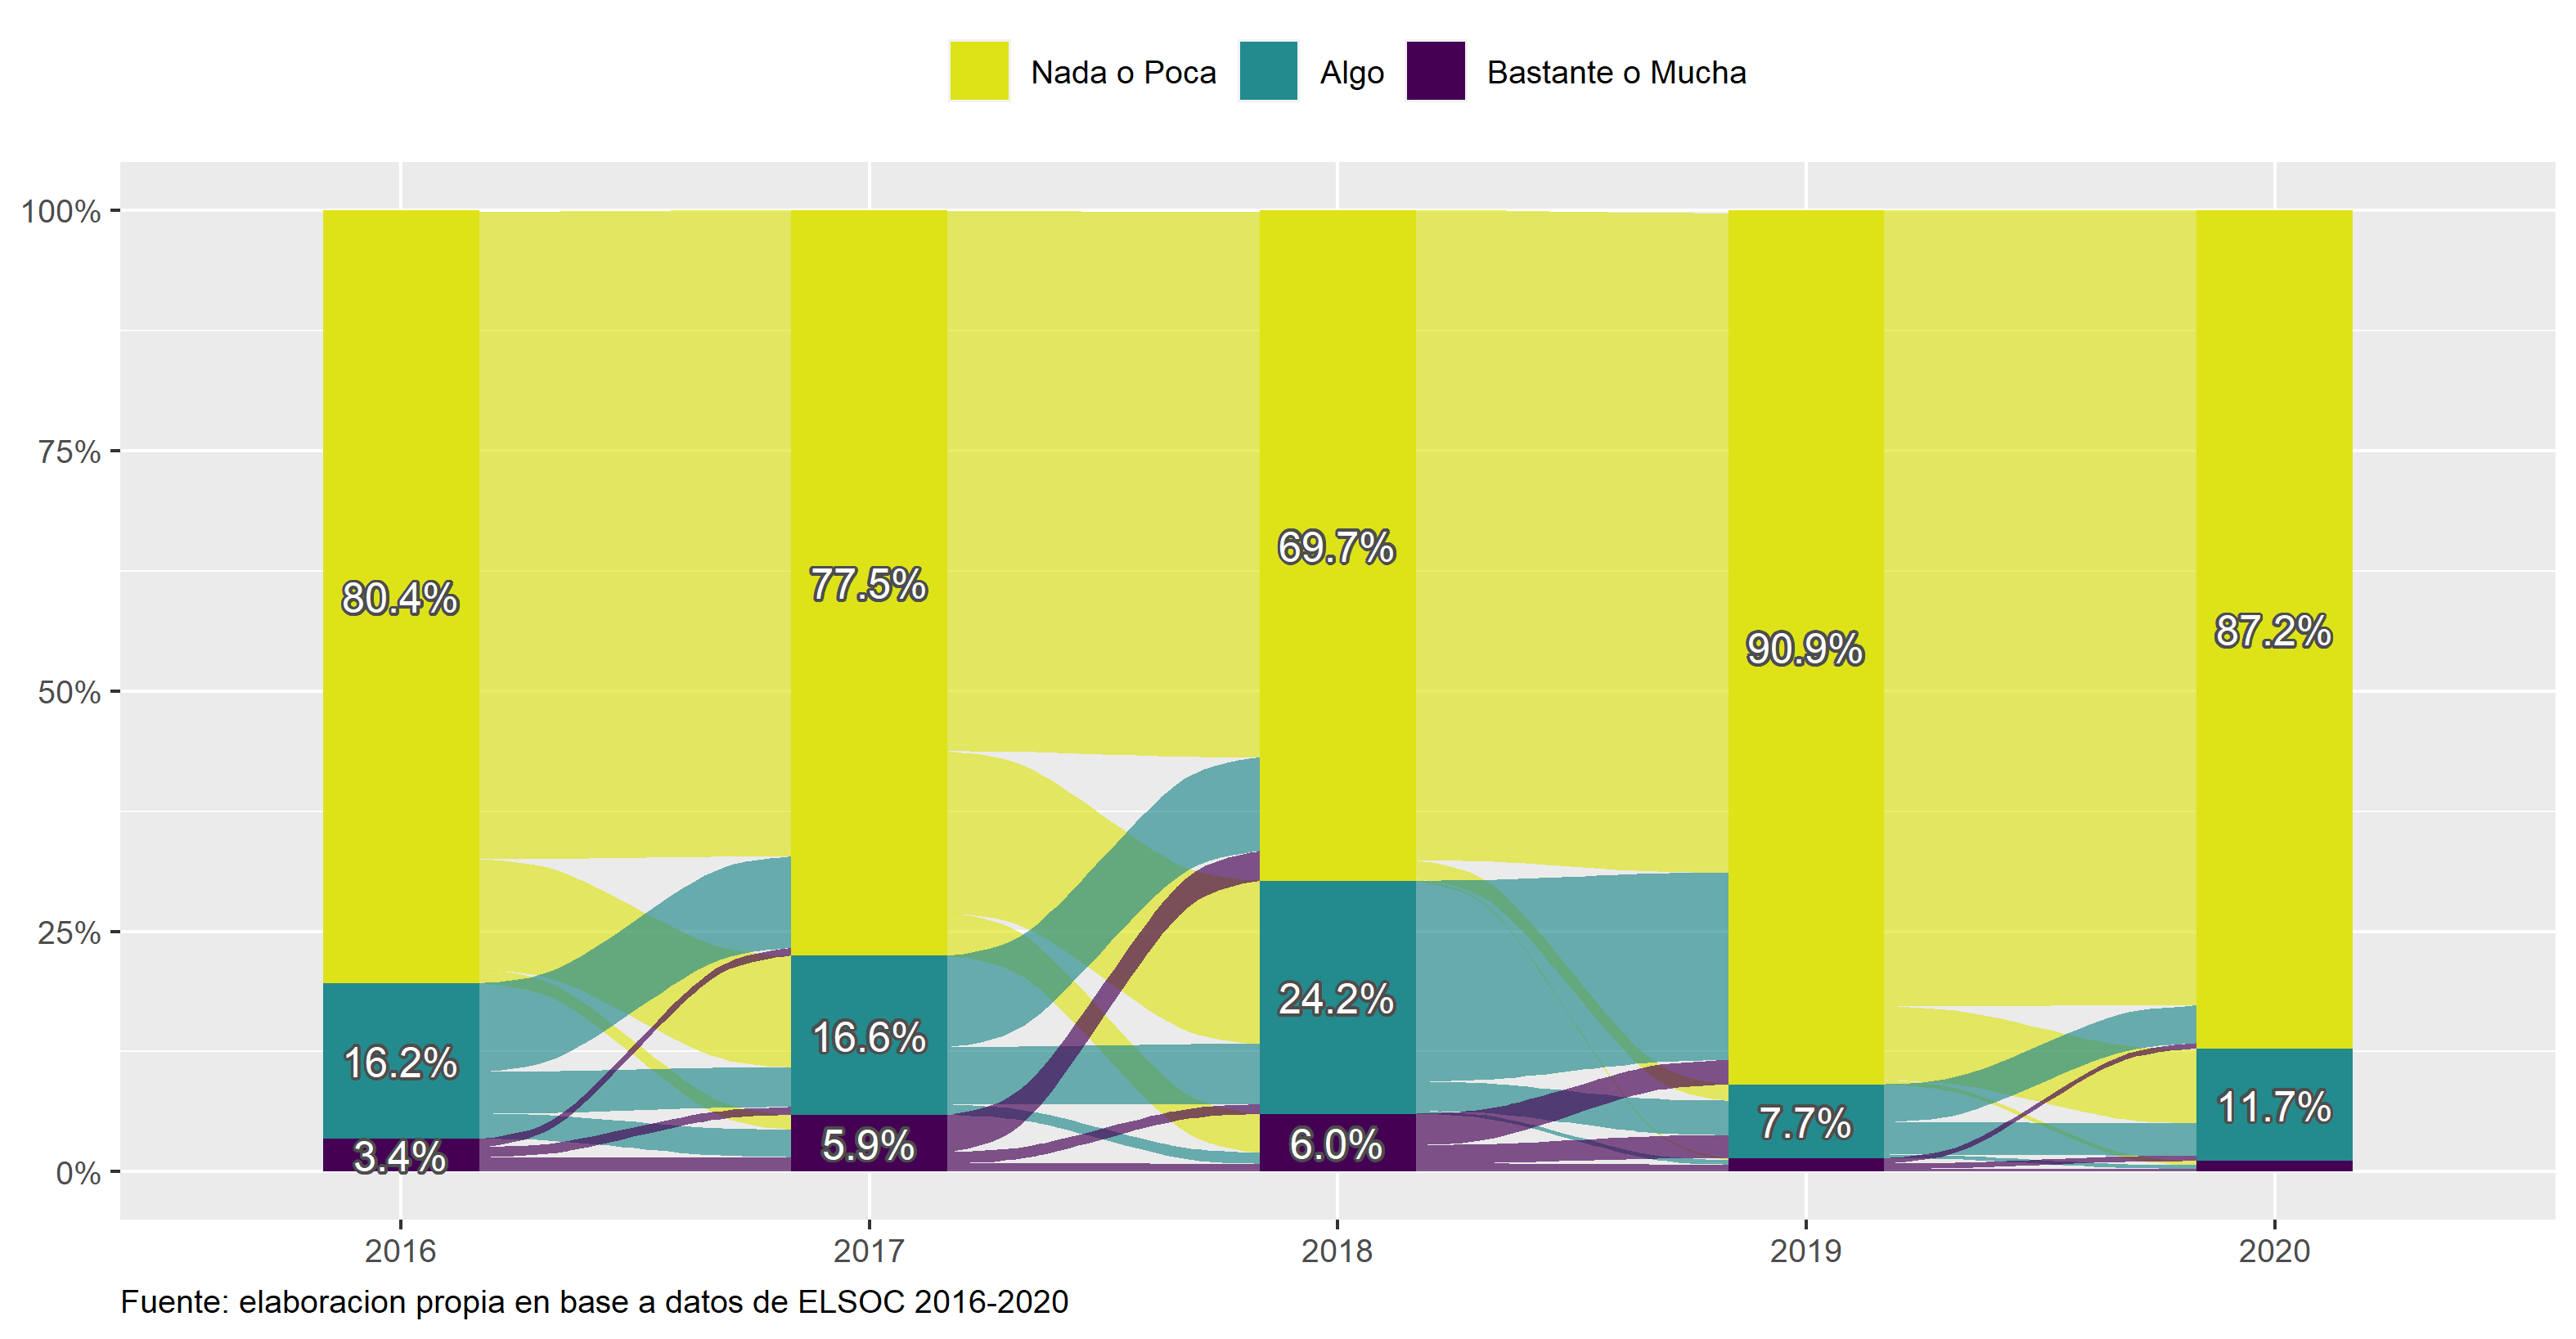
\includegraphics[width=1\linewidth,height=1\textheight]{output/graphs/alluvial_conf_institucional} 

}

\caption{Cambios en la subdimensión confianza institucional.}\label{fig:alluvial-conf-institucional}
\end{figure}

En general, al igual que para el ítem de confianza entre personas, en la Figura \ref{fig:alluvial-conf-institucional} se observa que el ítem de confianza institucional es muy reducido en Chile entre los respondentes, quienes mayoritariamente confían ``Nada o poco'' en las instituciones del país, en este caso el gobierno, el presidente o los partidos políticos. Era de esperarse, pero corresponde a una de las mayores brechas en la cohesión, con un aumento notorio en el 2019 (pasando de 70\% a un 91\%), antes de bajar nuevamente en 2020, pero de forma muy leve. El salto entre 2018 y 2019 es uno de los mayores observados en este capítulo, correspondiente al aumento del malestar de los ciudadanos frente a la ausencia de respuestas a sus demandas. Finalmente, la categoría ``Bastante o mucha'' confianza se mantiene muy baja en todas las olas, llegando a un máximo del 6\% en 2018, antes de bajar casi a cero en 2020.

En cuanto a las variaciones entre olas y entre respondentes, las personas desconfiadas mantienen masivamente su preferencia de un año a otro. Otro elemento de preocupación es que entre las personas que tenían ``Algo de confianza'' al inicio de la medición muestran en general una opinión poco estable de una ola a otra, con una fuga cada vez más importante hasta el 2018 hacia la categoría ``Nada o poca confianza''. Como era de esperarse, los cambios son nuevamente hacia categorías contiguas, con mínimos traspasos entre extremos.

En resumen, la confianza hacia las instituciones se ha degradado, lo que era esperable, pero a niveles críticos hasta la ola 2020.

\hypertarget{orientaciuxf3n-hacia-el-bien-comuxfan-1}{%
\section{Orientación hacia el bien común}\label{orientaciuxf3n-hacia-el-bien-comuxfan-1}}

\hypertarget{solidaridad}{%
\subsection{Solidaridad}\label{solidaridad}}

Los ítems que componen este indicador son

\begin{itemize}
\item
  Ha donado dinero a una obra social o de caridad
\item
  Ha prestado una suma de dinero de \$10.000.- o más
\item
  Ha conversado con una persona en problemas o deprimida
\item
  Ha ayudado a alguien a conseguir trabajo
\end{itemize}

\begin{figure}[H]

{\centering 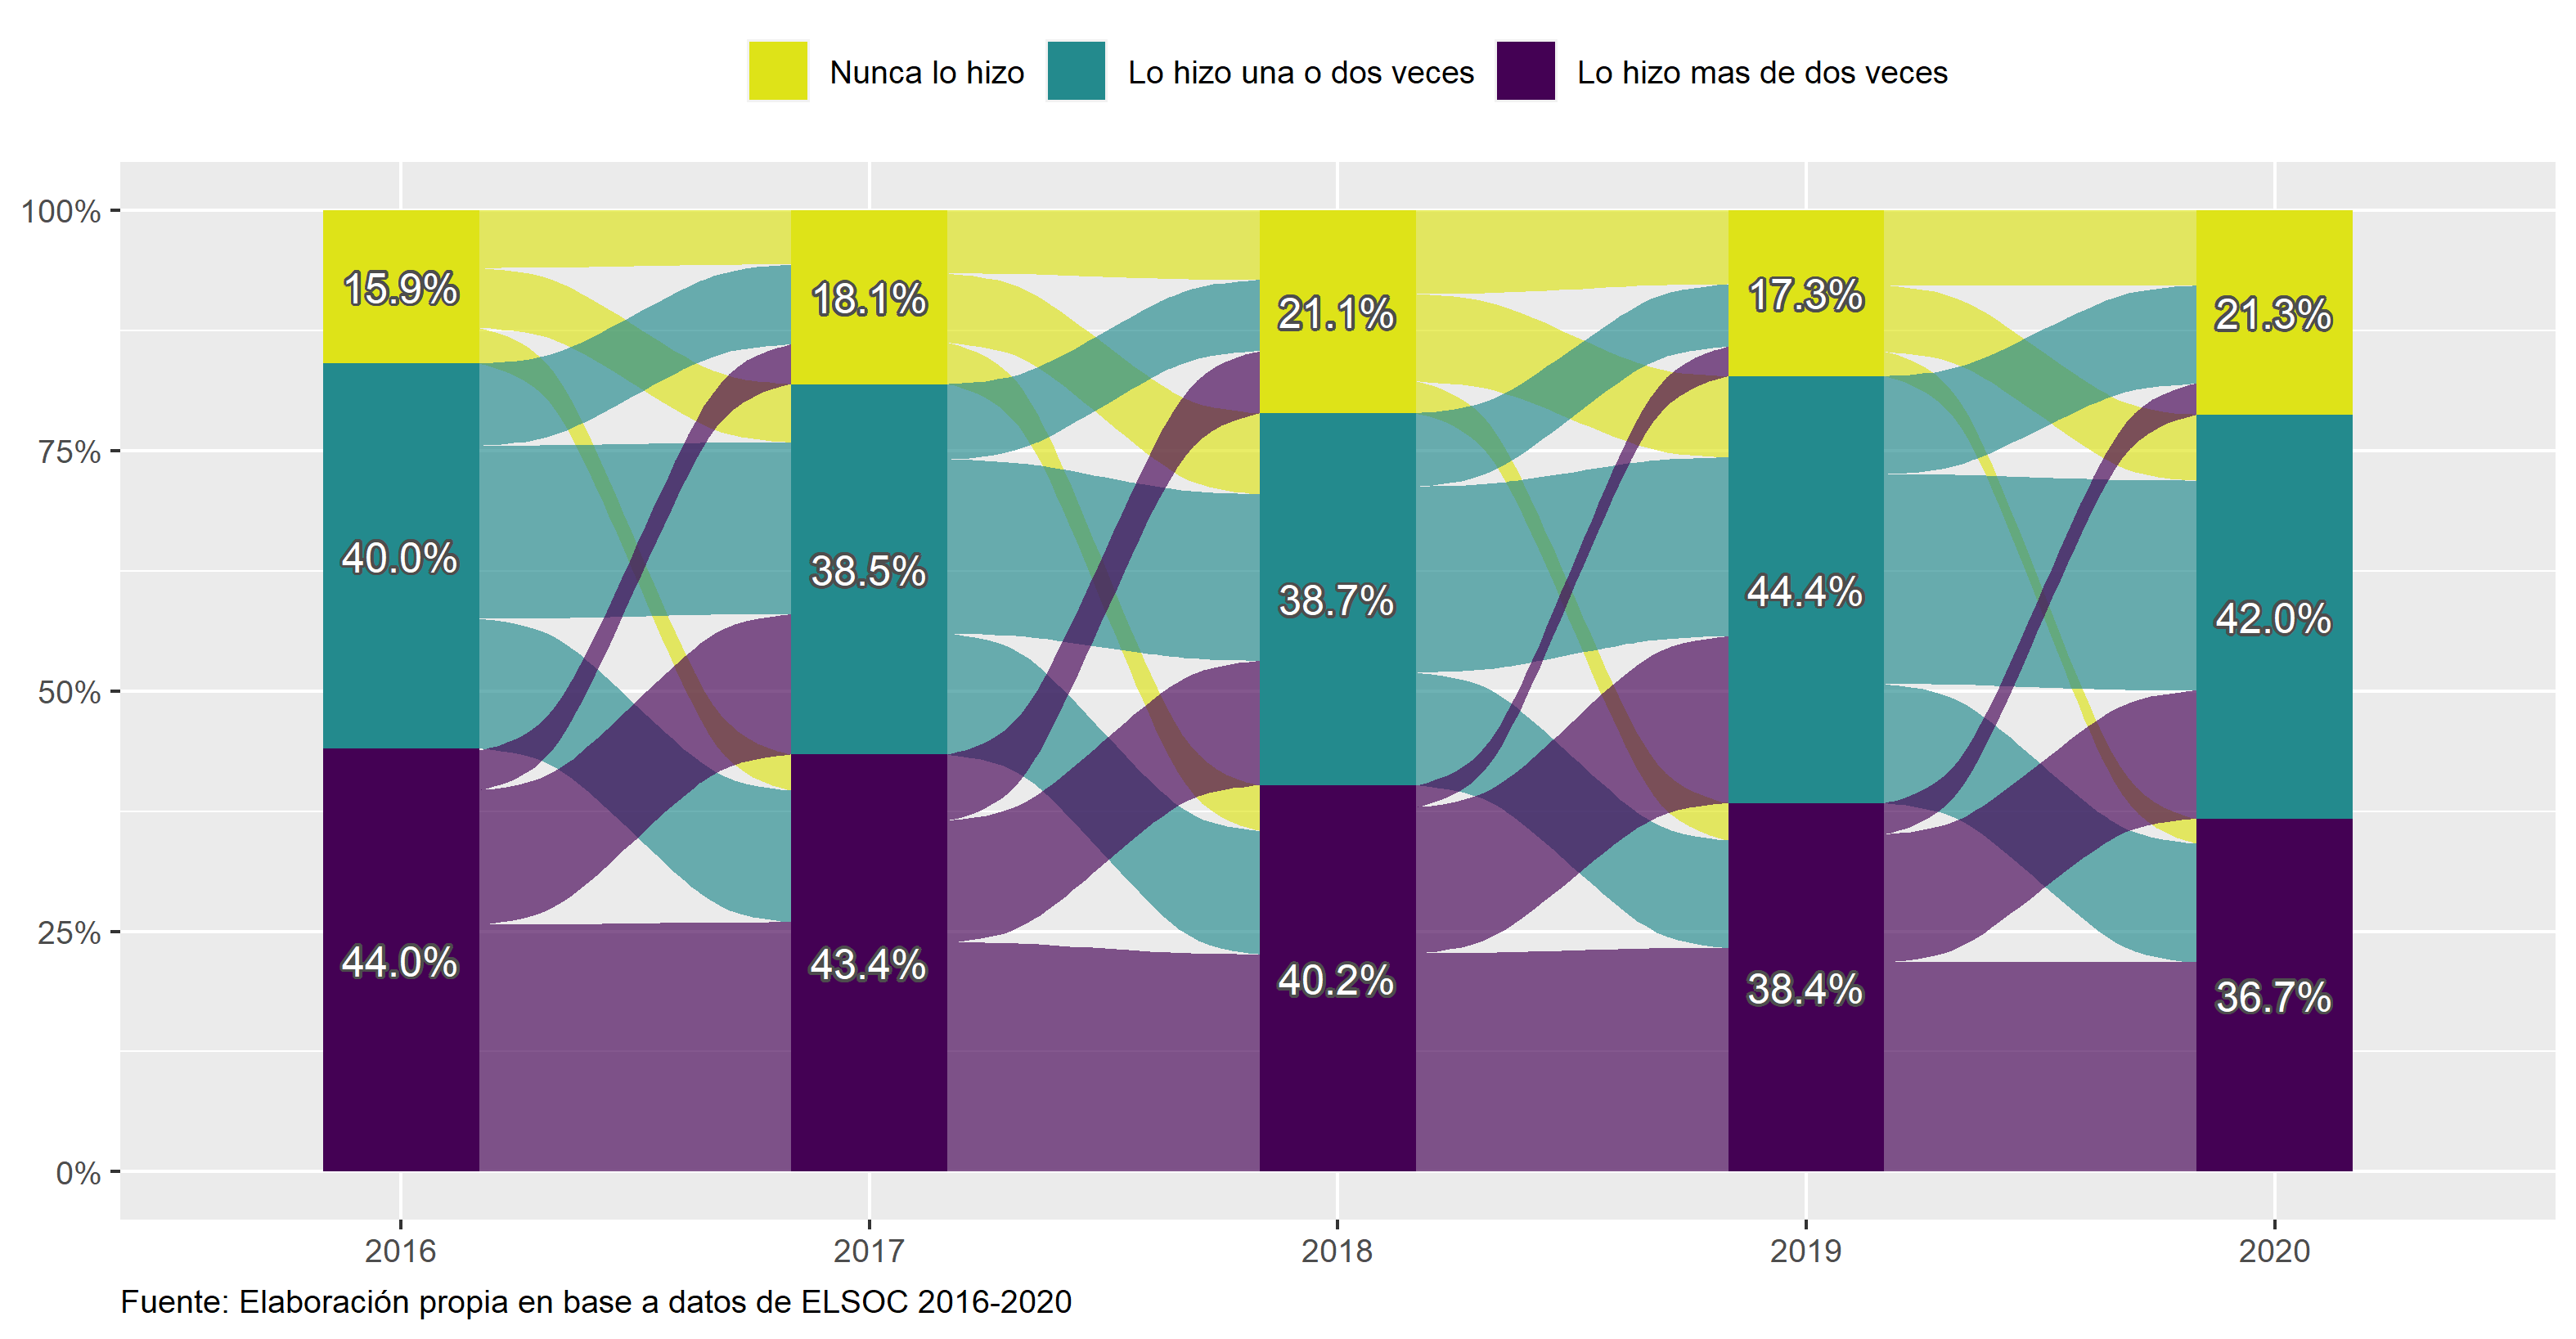
\includegraphics[width=1\linewidth,height=1\textheight]{output/graphs/alluvial_solidaridad} 

}

\caption{Cambios en la subdimensión solidaridad.}\label{fig:alluvial-solidaridad}
\end{figure}

En general, en el indicador que se observa en la Figura \ref{fig:alluvial-solidaridad} y que busca dar cuenta de la prosocialidad (visitas, donaciones, ayuda hacia otros) entre los respondentes, menos de un cuarto contesta que nunca ha tenido actividades prosociales, lo que se mantiene entre olas. Las categorías que indican una prosocialidad media (``lo hizo una o dos veces'') o alta (``lo hizo más de dos veces'') son casi equivalentes en las cinco olas. Solo presentan una pequeña variación hacia la baja en su tamaño general a lo largo del período. El estallido no significa un aumento para la ola 2020, aunque en mediano plazo, en 2016-2020, viene cayendo el porcentaje que fue solidario dos o más veces, lo que muestra una menor intensidad en los apoyos.

En cuanto a las variaciones entre olas y entre respondentes, la mayoría de los respondentes contesta lo mismo de una ola a otra, con flujos muy menores entre las dos categorías extremas. Los movimientos más importantes son hacia las categorías contiguas y estos flujos se mantienen muy estables a lo largo del período.

\hypertarget{participaciuxf3n-cuxedvica}{%
\subsection{Participación cívica}\label{participaciuxf3n-cuxedvica}}

Los ítems que componen este indicador son

\begin{itemize}
\item
  Firmado una carta o petición apoyando una causa
\item
  Asistido a una marcha o manifestación pacífica
\item
  Participado en una huelga
\item
  Usado las redes sociales para expresar su opinión en temas públicos
\end{itemize}

\begin{figure}[H]

{\centering 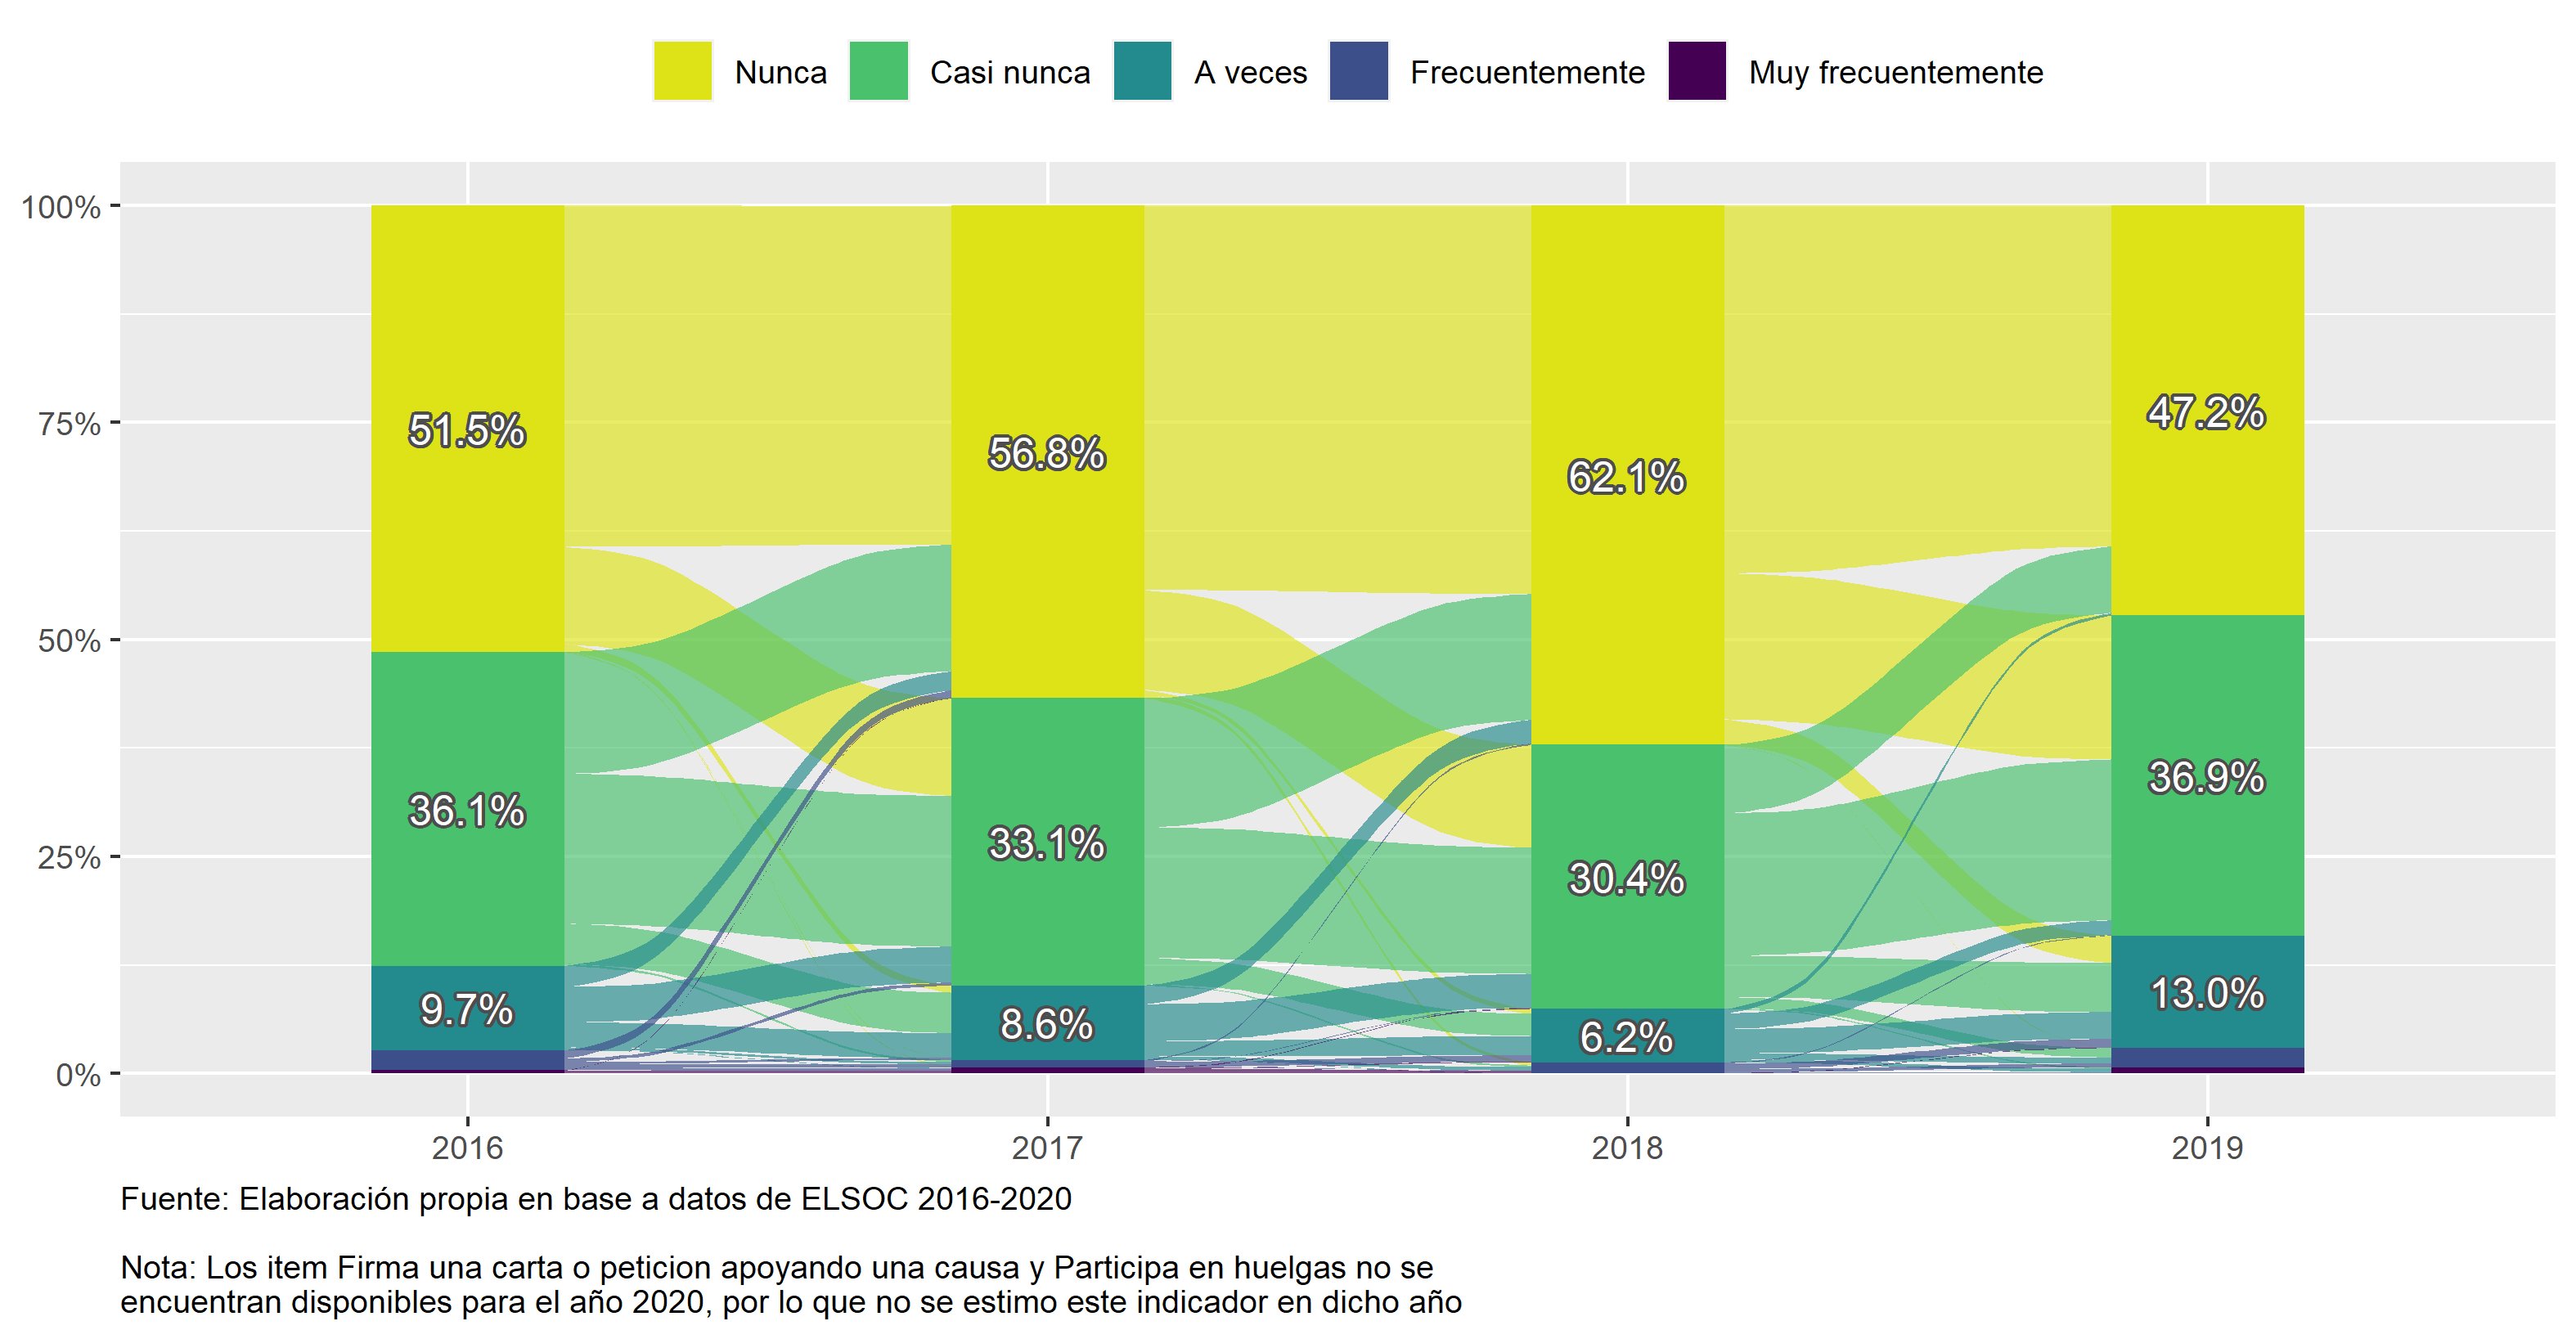
\includegraphics[width=1\linewidth,height=1\textheight]{output/graphs/alluvial_participacion} 

}

\caption{Cambios en la subdimensión participacion civica.}\label{fig:alluvial-participacion}
\end{figure}

En general, en la Figura \ref{fig:alluvial-participacion} se observa que en cuanto a la participación cívica (asistir a marchas, participar en huelgas, expresar opiniones por redes sociales y firmar una carta o petición), la mayoría de los respondentes nunca lo ha hecho, con un aumento constante de alrededor de un 55\% a un 60\% entre el 2017 y el 2018, antes de bajar nuevamente a su nivel inicial en 2019. Al no contar con los datos 2020, no podemos indicar si el estallido significó un cambio en esta nula participación cívica, como se podría esperar. La categoría ``casi nunca'' es la segunda de mayor importancia a lo largo del período con entre una cuarta y una tercera parte de las respuestas. Las opciones de participación cívica ``frecuente'' o ``muy frecuente'' son muy bajas, particularmente la última.

En cuanto a las variaciones entre olas y entre respondentes, la respuesta ``nunca'' es muy estable y presenta pocos cambios, siendo estos hacia la categoría contigua de ``caso nunca''. Este flujo aumenta levemente entre 2018 y 2019. Respecto de la categoría ``casi nunca'', los principales flujos son para la misma categoría al año siguiente, es decir que las personas mantienen su opinión o hacia la categoría contigua ``casi nunca''.

En resumen, fuera del aumento al doble en el período 2018-2019 de las categorías ``A veces'' y ``Frecuentemente'', que siguen siendo minoritarias, la participación cívica es muy baja y no varía particularmente entre olas.

\hypertarget{vuxednculos-territoriales}{%
\section{Vínculos territoriales}\label{vuxednculos-territoriales}}

Los items que componen este indicador son:

\begin{itemize}
\item
  Este barrio es ideal para mi
\item
  Me siento integrado/a en este barrio
\item
  Me identifico con la gente de este barrio
\item
  Este barrio es parte de mi
\end{itemize}

\begin{figure}[H]

{\centering 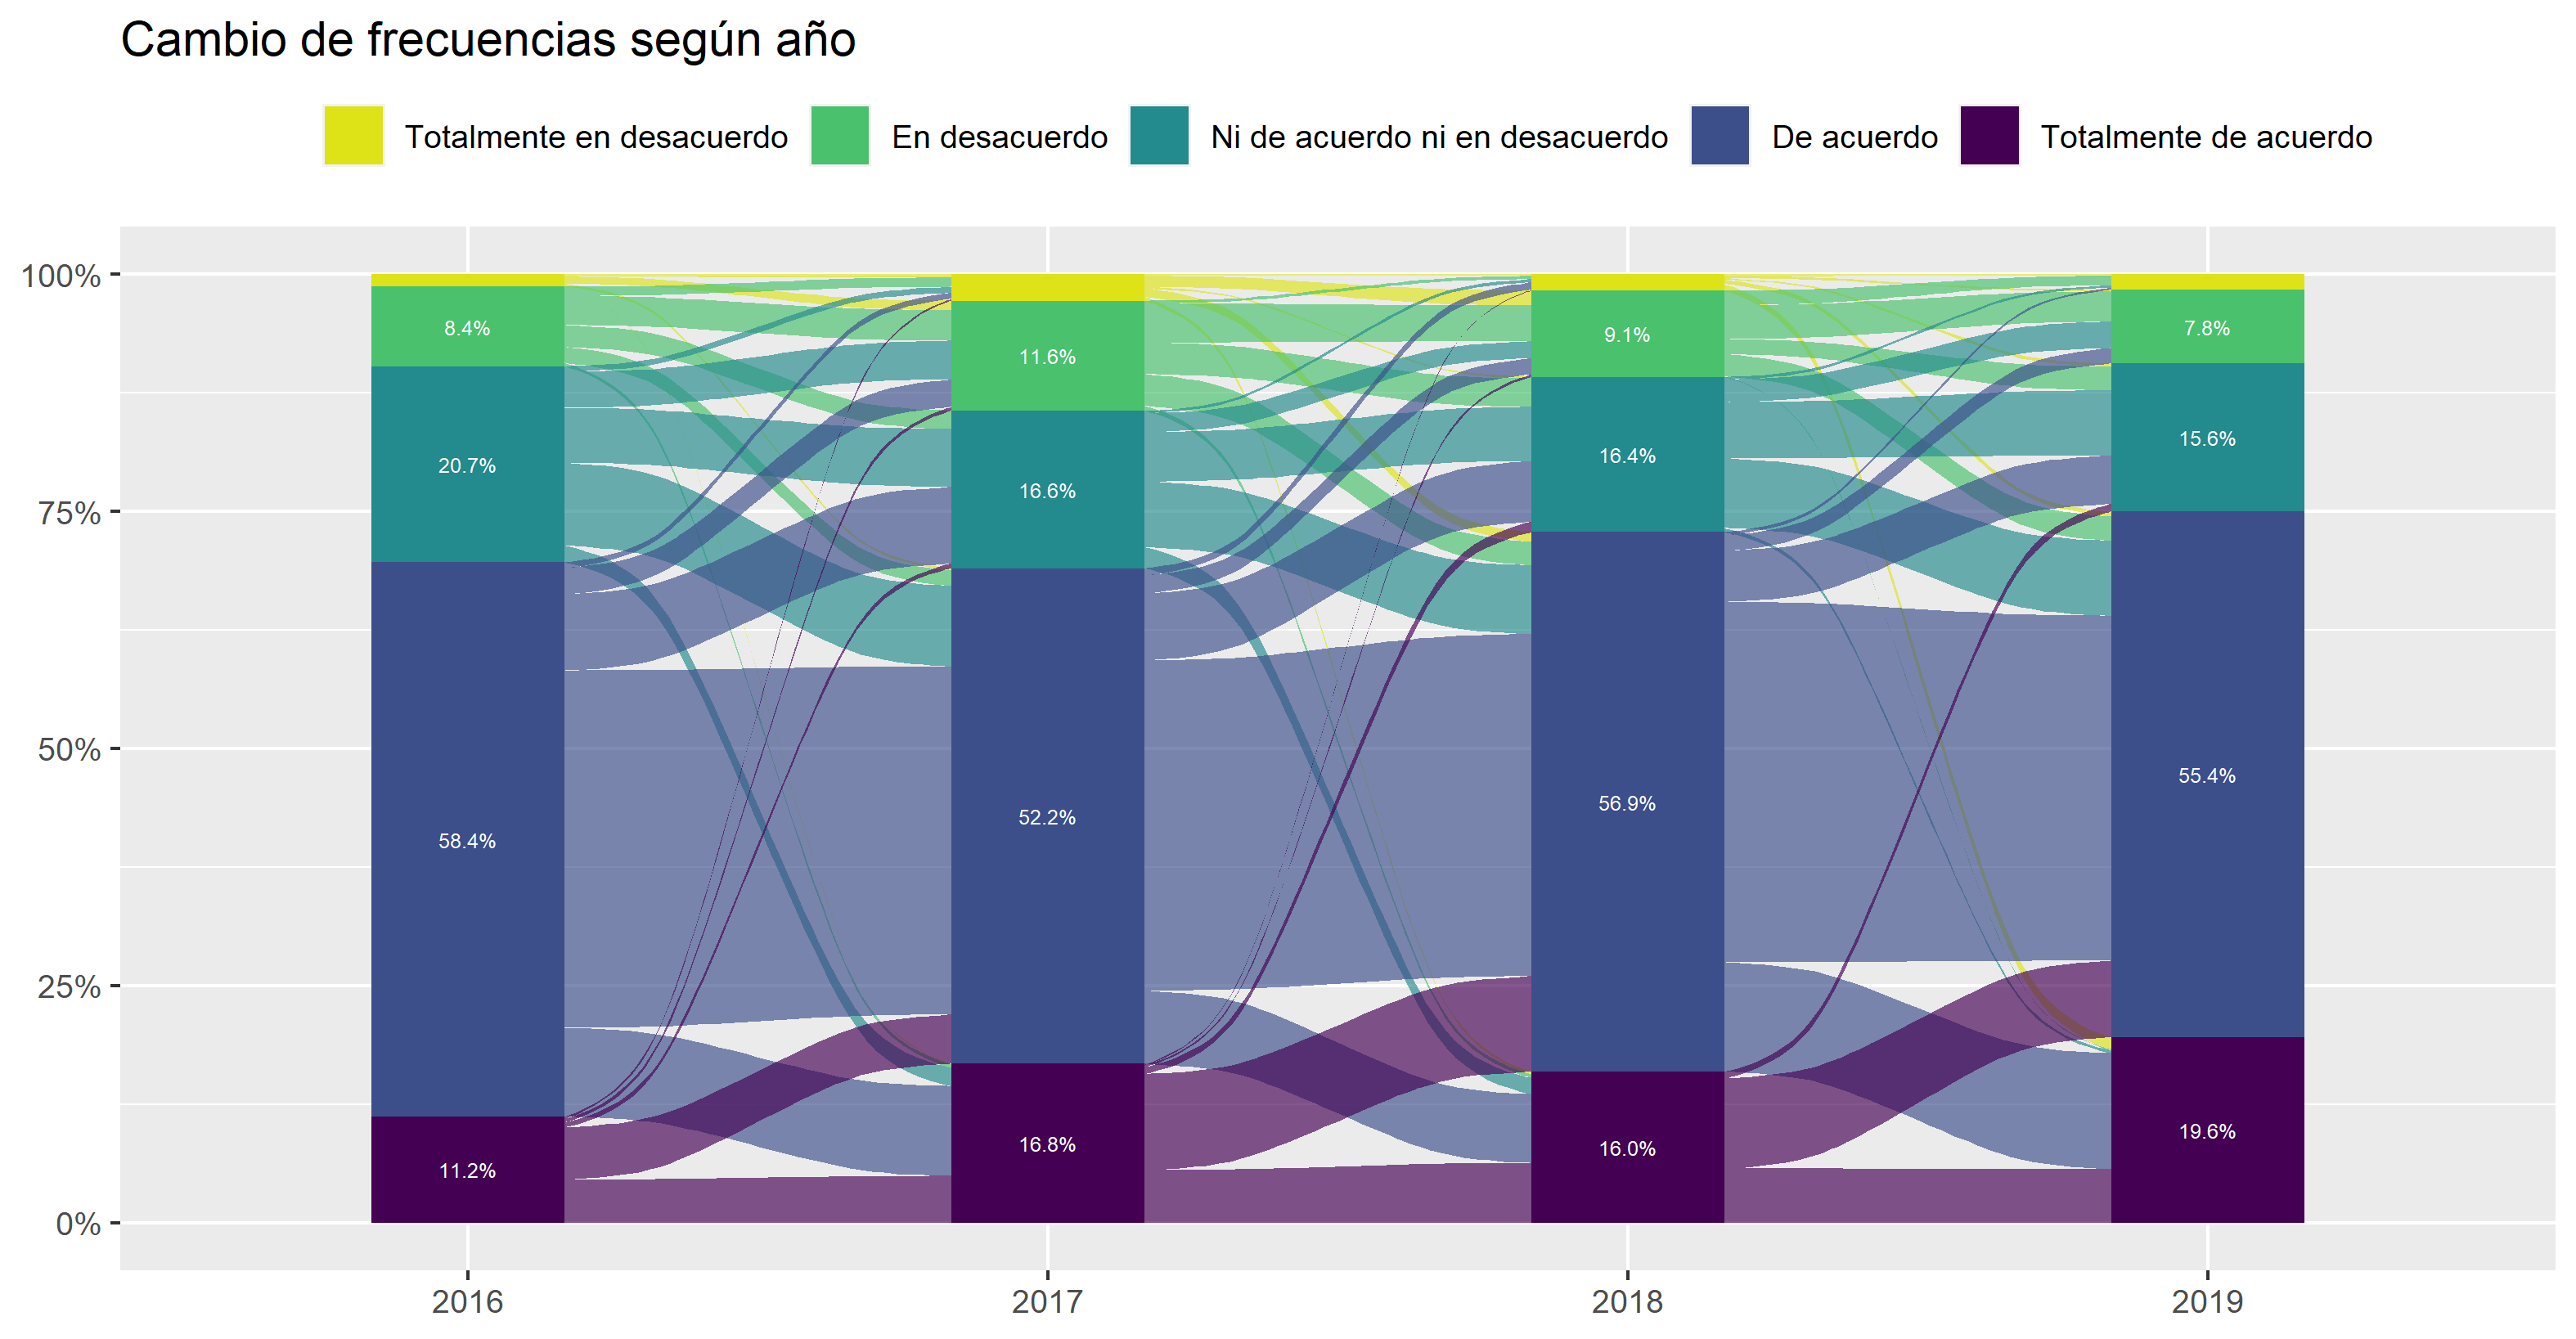
\includegraphics[width=1\linewidth,height=1\textheight]{output/graphs/alluvial_cohesion_territorial} 

}

\caption{Cambios en la subdimensión cohesion territorial.}\label{fig:alluvial-cohesion-territorial}
\end{figure}

En general, en la Figura \ref{fig:alluvial-cohesion-territorial} los respondentes suman una abrumadora mayoría entre ``de acuerdo'' respecto de su identificación con el barrio en que vive, opción que recoge casi el 60\% de las preferencias en todas las olas y ``totalmente de acuerdo'', con alrededor del 18\% en todas las olas, salvo en el 2016, cuando puntúa sólo un 11,2\%. Se trata de uno de los indicadores más positivos de cohesión social que analizamos en este capítulo. Una cantidad mínima de personas no se identifica con su barrio a lo largo de las cuatro olas. No contamos con los datos 2020, por lo que no se puede ver si el estallido tuvo un impacto sobre la identificación con el barrio aunque es esperable que no varíe particularmente.

En cuanto a las variaciones entre olas y entre respondentes, la categoría principal (``de acuerdo''), es decir de mayor identificación con el barrio, no conoce mayores flujos de un año a otro y es muy estable. Las demás categorías son más inestables e indican un mayor cambio de percepción entre olas, nuevamente hacia las categorías contiguas.

En resumen, también se trata de un indicador muy positivo de cohesión social, además de muy estable en el tiempo, aunque no se cuente con datos del 2020.

\hypertarget{conclusiuxf3n}{%
\section{Conclusión}\label{conclusiuxf3n}}

En primer lugar, respecto de las frecuencias, se observa una varianza más bien baja en las expresiones constitutivas de la cohesión social, desglosadas aquí en cuatro dimensiones principales (relaciones sociales de igualdad, sentido de pertenencia, orientación hacia el bien común, vínculos territoriales).

En cuanto a las frecuencias de los indicadores particularmente bajos, como era de esperarse, la desconfianza entre personas y hacia las instituciones es muy alta en Chile y varía muy poco en el período descrito, al igual que el número de contactos con diferentes ocupaciones y la percepción de justicia. Lo mismo ocurre con la prosocialidad. En especial, las personas confiadas o que piensan que en Chile se recompensa el esfuerzo representan un grupo muy limitado y esto constituye un inhibidor potente, aunque estable de la cohesión social y que no ha sido afectado por el estallido. Un factor alarmante es que, siendo baja la confianza hacia instituciones en Chile, logra aumentar la cantidad de personas que desconfían de ellas. Se entiende retrospectivamente por el contexto pre estallido, pero se trata de uno de los elementos de mayor preocupación para el caso de Chile, pues la degradación de este indicador ha llegado a niveles críticos.

Respecto de los indicadores medios, destaca el reconocimiento y respeto por la diversidad.

En cuanto a los indicadores altos, es notoria la alta identificación con Chile o el orgullo de ser chileno, pero se observa en esta dimensión una de las variaciones más notables en los gráficos analizados en este capítulo, en especial con una caída fuerte en 2019-2020 de la categoría de mayor identificación en las tres últimas olas, con una pérdida de 15 puntos. También destaca la alta identificación de los respondentes con el barrio en que viven, siendo uno de los indicadores más positivos de cohesión social, además de muy estable en el tiempo.

En segundo lugar, respecto de las varianzas, algunas casi no presentan alteraciones, como por ejemplo la confianza entre personas, hacia las instituciones o el reconocimiento y respeto por la diversidad. Lo mismo ocurre con la prosocialidad y los vínculos barriales.

En un punto intermedio, se encuentra la identificación con Chile, con variaciones entre respondentes sobre todo entre las categorías de mayor identificación con el país.

En cambio, el número de contactos con diferentes ocupaciones, las frecuencias varían significativamente de una ola a otra, lo que muestra una mayor volatilidad en el tipo de contactos de las personas. Ocurre lo mismo con la percepción de justicia, donde existen importantes cambios en las respuestas entre olas, siendo este indicador uno de los menos estables en el tiempo.

Se puede hipotetizar que la cohesión social cambia poco, pues de lo contrario no sostendría la sociedad, ni en tiempos de estallido social, pero algunos indicadores muestran la fragilidad de algunos de sus pilares, particularmente en la dimensión institucional. Ahora, luego de este análisis longitudinal de las principales dimensiones de la cohesión social, en la parte siguiente, se ofrecerá una visión sintética de la cohesión social a partir de las similitudes entre individuos y territorios. Nos centramos para ello en los diversos niveles de inclusión e integración de agrupaciones sociales en la sociedad chilena.

\hypertarget{habilitadores-e-inhibidores-de-la-cohesiuxf3n-social}{%
\chapter{Habilitadores e inhibidores de la cohesión social}\label{habilitadores-e-inhibidores-de-la-cohesiuxf3n-social}}

Los capítulos anteriores entregaron una medición de la cohesión social y mostraron su evolución en el tiempo. Basado en lo anterior, este capítulo ofrece un análisis de la cohesión social en Chile en relación a una serie de factores que en el marco del modelo conceptual de la CEPAL denominamos elementos habilitadores y/o ihnibidores de la cohesión social. La pregunta a abordar en este espacio es ¿Qué factores afectan los niveles de cohesión social? Antes de hablar sobre los factores, es necesario establecer una forma de analizar los indicadores de cohesión social para las nueve subdimensiones en consideración. Una posibilidad sin duda es analizar los factores en relación a cada una de las subdimensiones, pero esta estrategia tiene la desventaja de enfocarse en las subdimensiones por separado y perder de vista el tema central de este informe, que es la cohesión social como concepto macro. Por ello es que inicialmente generaremos una tipología de cohesión social, lo que nos permitirá identificar distintas clases o perfiles de personas en relación a sus puntajes en los distintos indicadores descritos en los capítulos anteriores. En base a esta tipología posteriormente analizaremos cómo los distintos perfiles se asocian a factores que habilitan o inhiben la cohesión, tales como educación, ingreso, situación laboral, entre otros.

\hypertarget{perfiles-de-cohesiuxf3n-social}{%
\section{Perfiles de cohesión social}\label{perfiles-de-cohesiuxf3n-social}}

La construcción de perfiles o tipos en el análisis de datos posee distintas aproximaciones, que en términos simplificados podemos resumir en dos: diferenciación de niveles y diferenciación de perfiles o tipos. En el caso de los niveles, una estrategia posible sería promediar el puntaje de todos los indicadores y categorizar a las personas en niveles estableciendo ciertos puntajes de corte, por ejemplo ``alto'' quienes poseen puntaje superior al promedio, y ``bajo'' a aquellos que puntuan igual o bajo el promedio. Esta aproximación tiene la ventaja de ser muy simple, pero desconoce las posibles diferencias sistemáticas en las respuestas de las personas. Por ejemplo, en el caso de tener dos indicadores, una persona que posee alto puntaje en uno y bajo en otro obtendrá el mismo puntaje que otra persona que tiene puntajes inversos en los mismos indicadores. Con el objetivo de poder dar mejor cuenta de los puntajes de los respondentes a una serie de variables o indicadores es que se utiliza la segunda alternativa: diferenciación de perfiles de respuesta. Para ello, se estiman modelos que intentan representar a la mayoría de los patrones de respuesta existentes, siendo cada uno de estos patrones genéricos un perfil o clase. El resultado del análisis consiste en la agrupación de individuos semejantes entre sí, pero diferentes de otros, por lo que reflejan niveles o formas de cohesión diversas.

Los procedimientos de clasificación automática en pefiles de respuestas comparan sistemáticamente los niveles de respuesta entre individuos utilizando una medida de distancia que establece su similitud. Para generar los tipos en el presente capítulos utilizaremos el análisis de clases latentes (ACL) (\protect\hyperlink{ref-collins_latent_2010}{Collins \& Lanza, 2010}). En términos simples, este procedimiento de estimación supone que los niveles observados en los patrones de respuesta son generados por una variable subyacente con dos o más clases. El ACL ubica la clasificación en el marco de los modelos de ecuaciones estructurales, por lo que la estimación maximiza la probabilidad de que un individuo pertenezca a una clase. Con este análisis se obtienen dos estimaciones principales: la probabilidad de pertenencia a la clase dado el puntaje en el indicador, y el tamaño de cada una de las clases.

El procedimiento incorpora una dimensión longitudinal pues considera todas las mediciones disponibles en las distintas olas del panel. Aunque lo anterior reduce la cantidad de casos a quienes respondieron en todas las olas, ofrece mayor estabilidad en la estimación.

La estimación con ACL para los indicadores de cohesión social utiliza las variables observadas dentro de cada una de las dimensiones en todas las olas del panel. Se procedió a calcular las medias de los ítemes que componen cada una de las 9 subdimensiones en cada año; posteriormente se calculó la media de las subdimensiones en todos los años, obteniendo un puntaje para cada respondente en cada subdimensión. Las medias de las subdimensiones fueron dicotomizadas usando la mediana como punto de corte. El análisis de clases latentes considera entonces nueve variables dicotómicas que describen los individuos en términos de alto o bajo puntaje en cada subdimensión de la cohesión social.

El procedimiento sugerido de estimación de ACL es generar modelos con distinto número de clases y comparar sus estadísticos de ajuste. Lueog de realizar estas estimaciones, el modelo que resultó con mejor ajuste fue el de tres clases. En base a este número es posible representar gráficamente la estructura de cada clase según sus niveles (o probabilidad de pertenencia a la clase) en cada una de las subdimensiones, tal como se presenta en la Figura \ref{fig:clases-latentes}:

\begin{figure}[H]

{\centering 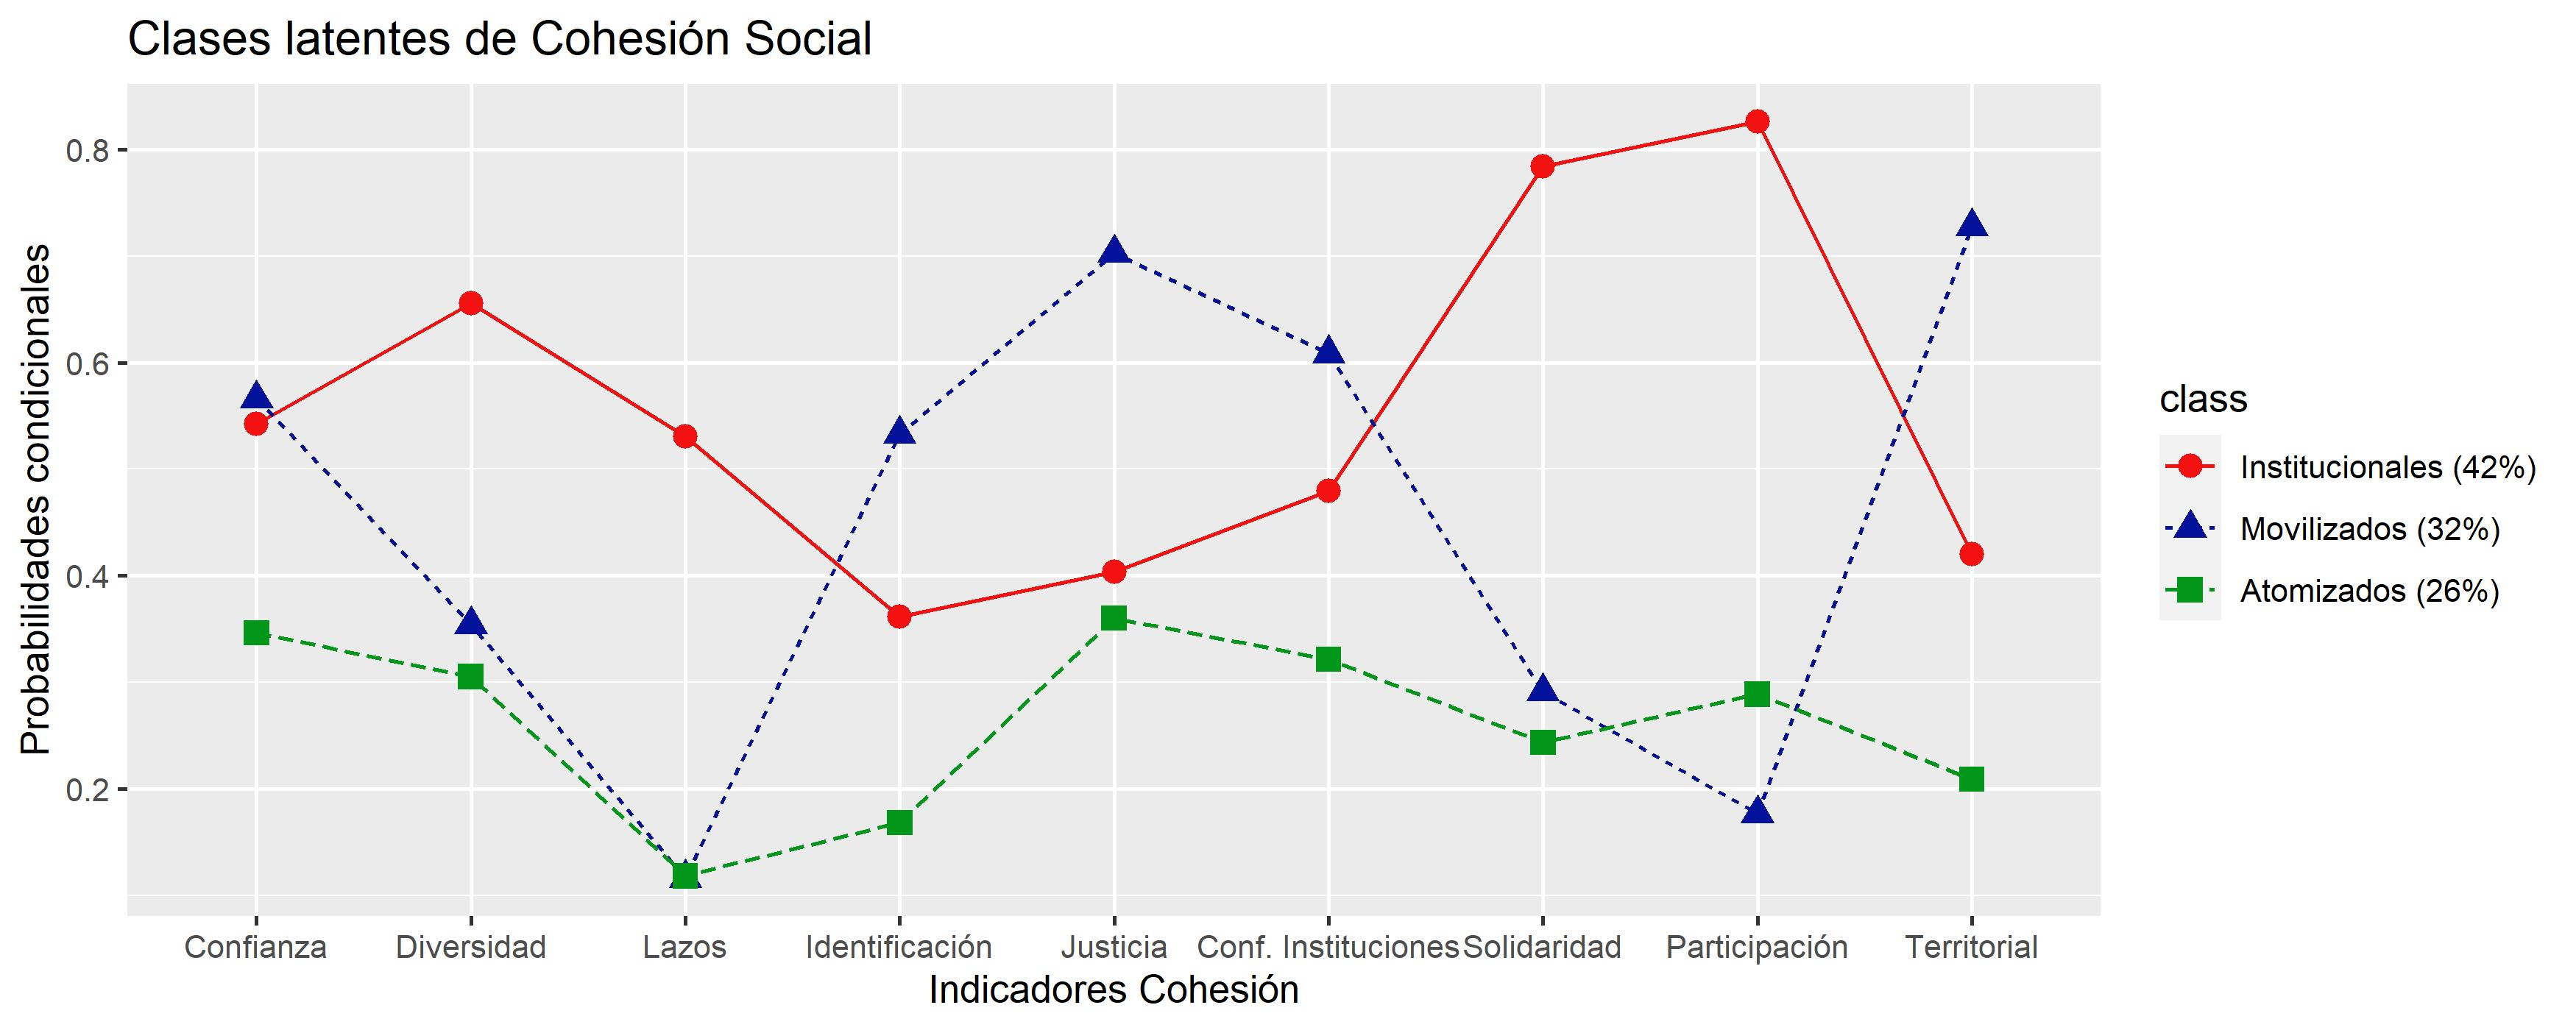
\includegraphics[width=1\linewidth,height=1\textheight]{output/graphs/lca3} 

}

\caption{Tipologia de las clases latentes de cohesion social.}\label{fig:clases-latentes}
\end{figure}

En el gráfico de la Figura \ref{fig:clases-latentes} observamos en el eje X a las distintas subdimensiones de cohesión social del modelo de la CEPAL más la dimensión territorial añadida para este trabajo. Por temas de mayor claridad en el gráfico incluimos a la dimensión territorial junto a las otras subdimiensiones que corresponden a la dimensión de pertenencia. Las tres líneas identifican a cada una de las clases y su nivel (probabilidad) de respuesta en cada indicador. Las clases fueron luego etiquetadas para dar un sentido sustantivo a cada perfil, donde tenemos Movilizados, Institucionales y Atomizados, que se describen a continuación

\begin{itemize}
\tightlist
\item
  Movilizados:
\end{itemize}

Comprenden 42\% de la muestra, siendo la clase identificada de mayor tamaño. Los elementos que les destacan remiten a una dimensión horizontal de la cohesión social en la cual los principios de cooperación y respeto entre iguales operan como organizadores de la vida social. Se caracterizan por sus conductas prosociales, orientadas al altruismo y la solidaridad, así como su activa participación cívica y mayor respeto a la diversidad de minorías visibles. Se diferencia de los institucionales porque, sin llegar a los niveles del grupo atomizado, se identifica menos con el país, cree que no hay justicia en la distribución de recompensas sociales y posee menor confianza en instituciones.

\begin{itemize}
\item
  conductas prosociales orientadas al altruismo y la solidaridad
\item
  activos en participación cívica
\item
  Altos en respeto a la diversidad cultural
\item
  bajos en los indicadores que caracterizan a los institucionales
\item
  Institucionales.
\end{itemize}

Comprenden 32\% de la muestra. Sus características refieren a una forma de cohesión vertical o jerarquizada, en la cual las instituciones y la identificación nacional organizan el comportamiento individual. Se identifican fuertemente con el país, donde perciben que operan principios de justicia fundados en el mérito, confían en las instituciones y son apegados al barrio. Son menos tolerantes a la diversidad social, aislados socialmente, muestran menor solidaridad y baja probabilidad de participación cívica.

\begin{itemize}
\item
  Identificación con el país
\item
  Creen que en Chile las personas son recompensadas por su inteligencia y su esfuerzo
\item
  Exhiben un nivel comparativamente alto de confianza en las instituciones
\item
  más altos en confianza vecinal
\item
  bajos en lazos y participación
\item
  Atomizados:

  Presentan los niveles más bajos en todas las subdimensiones y comprenden 26\% de esta muestra. Destacan la carencia de lazos sociales, así como sus bajos niveles de identificación y solidaridad.
\end{itemize}

\hypertarget{perfiles-de-cohesiuxf3n-social-en-el-territorio-nacional}{%
\section{Perfiles de cohesión social en el territorio nacional}\label{perfiles-de-cohesiuxf3n-social-en-el-territorio-nacional}}

Antes de comenzar con el análisis de factores habilitadores de la cohesión social resulta interesante explorar la distribución territorial de los perfiles de cohesión social. Esto permite apreciar la pauta predominante en cada región del país, como se muestra en la Tabla \ref{tab:clases-region}. Debido a que la muestra ELSOC es de carácter nacional, y no busca representación regional, la Tabla \ref{tab:clases-region} presenta 13 regiones, pero el análisis se concentra en seis que poseen casos suficientes.

\label{tab:clases-region}Distribucion de las clases de cohesion social por region

Region

Clases de cohesión social

Movilizados

Institucionales

Atomizado

N=100\%

Tarapaca

54.5

27.3

18.2

22

Antofagasta

60.0

25.7

14.3

35

Atacama

51.9

22.2

25.9

54

Coquimbo

28.2

42.4

29.4

85

Valparaiso

46.4

28.1

25.4

224

Metropolitana

47.8

26.6

25.6

425

Lib. Gral. B. Ohiggins

56.6

20.8

22.6

53

Maule

38.8

38.8

22.3

121

Bio Bio

37.8

38.2

24.0

275

Araucania

36.4

39.7

24.0

121

Los Rios

12.9

74.2

12.9

31

Los Lagos

48.5

30.3

21.2

33

Aysen

63.6

18.2

18.2

11

La distribución de los perfiles en cada región es marcadamente diferente, pero no es posible identificar pautas claras que asocien las características de los territorios con los perfiles de cohesión social. De todas formas, siete de las 13 regiones poseen un número de casos que no asegura representación, por lo que los resultados no se elaboran en su totalidad.

En el perfil de cohesión horizontal que denominamos ``movilizados'', ocho regiones se encuentran por sobre la media nacional de este perfil. Destacando la Región Metropolitana (47.8\%) y de Valparaíso (46.4). La región de Coquimbo (28.2\%) presenta el valor más bajo en esta dimensión.

En el perfil de cohesión vertical que denominamos ``institucional'', cinco regiones se encuentran por sobre la media nacional de este perfil, cuatro de ellas con suficientes casos, destacando Coquimbo (42.4\%). El nivel más bajo en este perfil se encuentra en la región Metropolitana (26.6\%), no demasiado alejado de la media nacional.

El perfil atomizado presenta valores próximos a la media en las regiones con mayor número de casos, encontrándose su nivel más alto en Coquimbo (29.4\%) y el más bajo en Maule (22.3\%).

\begin{figure}[H]

{\centering 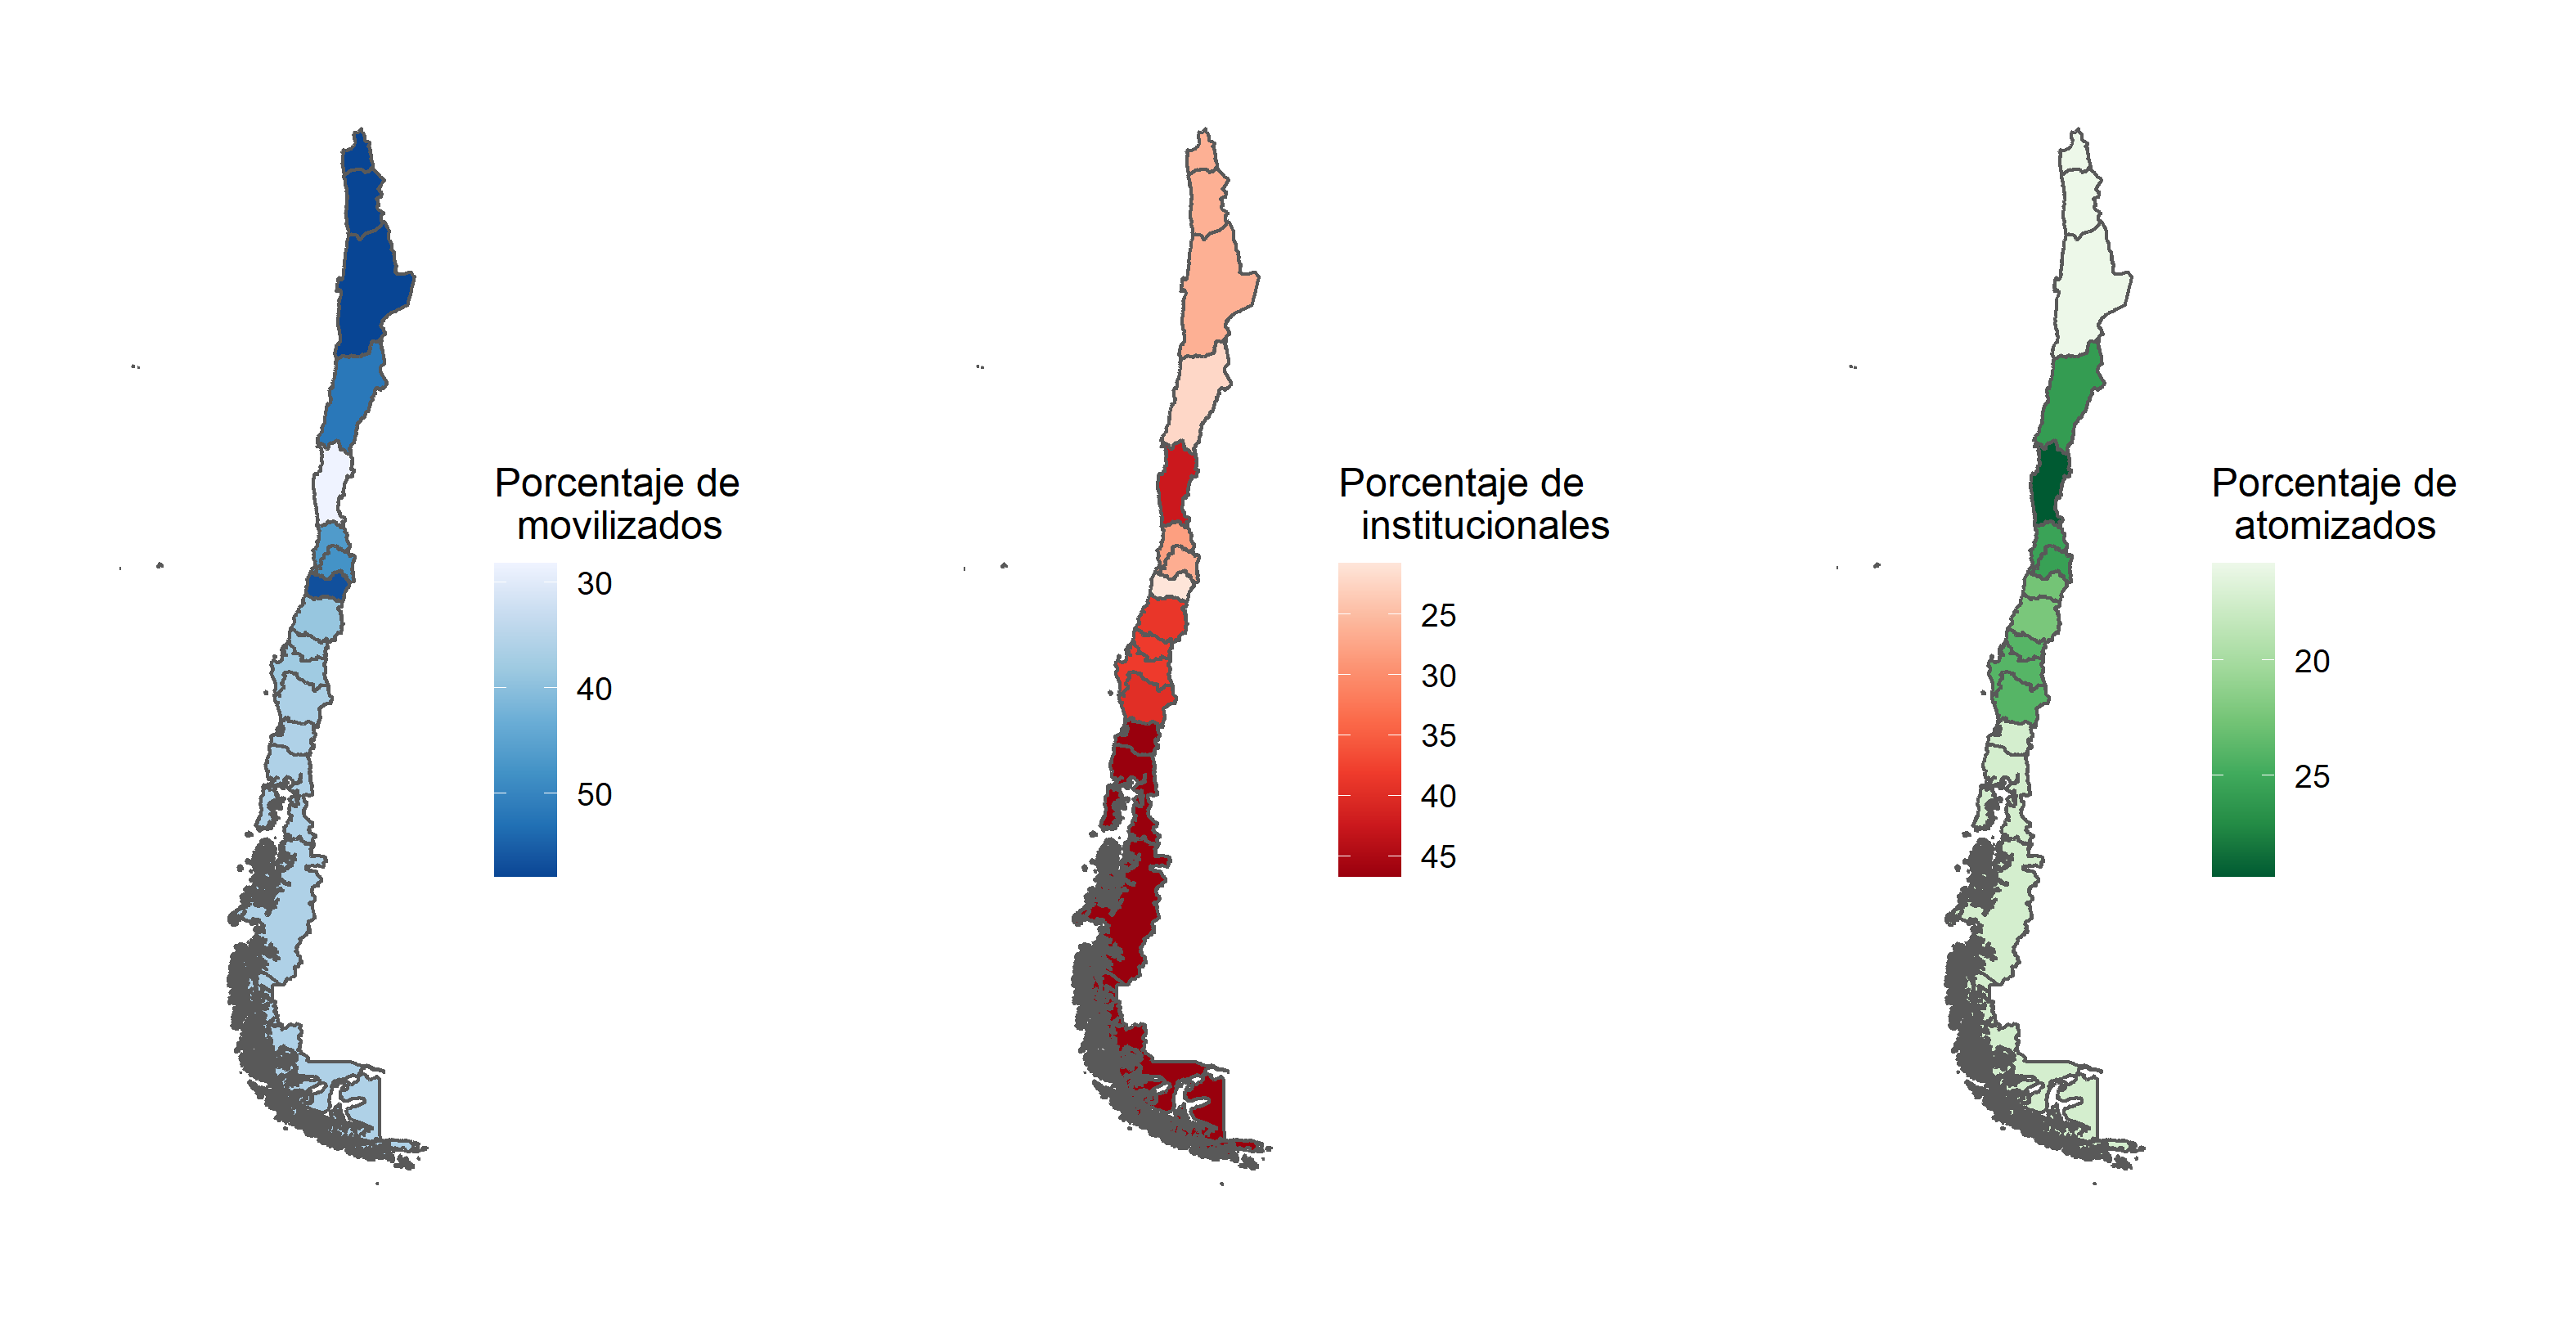
\includegraphics[width=1\linewidth,height=1\textheight]{output/graphs/mapas_region} 

}

\caption{Mapa de la istribución de las clases latentes de cohesion social por region.}\label{fig:mapas-region}
\end{figure}

La Figura \ref{fig:mapas-region} muestra gráficamente la distribución de la intensidad de las tipologías de clases latentes en las distintas regiones del país. Debido a que la muestra utilizada en este informe no incluye casos para todas las regiones y en algunas se posee una muestra pequeña, estos casos fueron agrupados. Específicamente, se agruparon a) las regiones de Tarapacá, Antofagasta y Arica y Parinacota; b) Bio Bio y Ñuble; y c) Los Ríos, Los Lagos, Aysén y Magallanes.

\hypertarget{perfiles-de-cohesiuxf3n-seguxfan-elementos-habilitadores}{%
\section{Perfiles de cohesión según elementos habilitadores}\label{perfiles-de-cohesiuxf3n-seguxfan-elementos-habilitadores}}

Las tres clases de cohesión social estimadas previamente permiten agrupar individuos con perfiles de cohesión similares, para describirles en términos de las características de su inclusión social. Los elementos de inclusión son el área preferente de implementación de las políticas públicas y pueden concebirse como habilitadores o disruptores de la cohesión social. Cepal (fc:42) comprende la cohesión social volcada a la igualdad como ``la capacidad de una sociedad y sus instituciones democráticas de promover relaciones sociales de igualdad y generar un sentido de pertenencia y una orientación hacia el bien común de una forma percibida como legítima por sus miembros.'\,' Esta definición multidimensional resalta la igualdad en las relaciones sociales, el sentido de pertenencia, la orientación hacia el bien común y la legitimidad democrática. La definición describe un proceso e incorpora un elemento normativo destinado a orientar las políticas públicas, consistente con el marco establecido por la Agenda 2030. La habilitación se refiere a elementos de la estructura social (inclusión) que favorecen la orientación de un modelo de cohesión volcado a la igualdad. El proceso de la cohesión social puede también enfrentar disrupciones ya sea estructurales, como exclusión persistente, o coyunturales como los ciclos económicos o recientemente la pandemia asociada al covid-19.

Los factores habilitadores están clasificados en siete grupos: inclusión laboral, edad, educación, nivel de ingreso, etnia, nacionalidad, aislamiento territorial.

\hypertarget{inclusiuxf3n-laboral}{%
\subsection{Inclusión laboral}\label{inclusiuxf3n-laboral}}

El acceso al mercado de trabajo se encuentra estrechamente asociado con el bienestar de las personas. En efecto, la superación de la pobreza depende en gran medida de la inserción laboral. En América Latina, Chile no es una excepción, las condiciones de trabajo informal, asociadas con pobreza y precariedad comprenden una parte significativa de la fuerza de trabajo. Las inserciones más débiles en el mercado de trabajo podrían afectar negativamente los niveles de cohesión social. El empleo formal comprende a los ocupados que cumplen con cualquiera de las siguientes condiciones: no poseen contrato laboral, no emiten boletas o facturas, no poseen cobertura de salud, no se encuentran cotizando para su pensión de retiro.

\label{tab:tabla-empleo}Efecto del tipo de empleo sobre las clases de cohesion social

Tipo de empleo

Clases de cohesión social

Formal

Informal

Movilizados

55.7

43.6

Institucionales

23.5

34.1

Atomizado

20.8

22.3

N=100\%

592.0

314.0

En la Tabla \ref{tab:tabla-empleo} se muestra que en el empleo formal la clase con mayor proporción es la movilizada. Si bien los informales también son mayoritariamente movilizados (43,6\%), en ellos aumenta considerablemente la proporción de la clase institucional (34.1\% vs 23.5\%).

\hypertarget{inclusiuxf3n-social}{%
\subsection{Inclusión social}\label{inclusiuxf3n-social}}

Hay diversas dimensiones en las brechas de participación en las condiciones de vida que una sociedad ofrece a sus integrantes.

\begin{itemize}
\tightlist
\item
  La etapa de \textbf{transición demográfica} en que se encuentra Chile muestra un peso creciente de los adultos mayores, quienes enfrentan condiciones de vida difíciles, por lo que se podría esperar pautas distintivas de cohesión social entre ellos. La Tabla \ref{tab:clases-edad} presenta los perfiles de cohesión según grupos de edad
\end{itemize}

\label{tab:clases-edad}Efecto de la edad sobre las clases de cohesion social

Grupos de edad

Clases de cohesión social

Entre 18 y 29

Entre 30 y 39

Entre 40 y 49

Entre 50 y 59

Mas de 60

Movilizados

66.3

57.0

49.6

39.7

21.8

Institucionales

9.1

14.3

27.7

35.2

57.2

Atomizado

24.6

28.7

22.7

25.1

21.0

N=100\%

175.0

286.0

264.0

375.0

390.0

El perfil de cohesión movilizada es más probable de encontrar en edades más jóvenes, disminuyendo de manera sostenida a medida que se incrementa la edad. Lo contrario ocurre con la cohesión institucional, que es más probable de aparecer a medida que aumenta la edad. Aunque los datos corresponden a un panel, por el breve periodo que cubre, no es posible establecer si este efecto se debe al paso del tiempo o corresponde a efectos de tipo generacional.

\begin{itemize}
\tightlist
\item
  El \textbf{sexo} de las personas afecta sus posibilidades de inclusión atendiendo a las pautas de roles asociadas con una sociedad patriarcal.
\end{itemize}

\label{tab:clases-sexo}Efecto del sexo sobre las clases de cohesion social

Sexo

Clases de cohesión social

Hombre

Mujer

Movilizados

47.7

40.8

Institucionales

31.7

33.0

Atomizado

20.6

26.2

N=100\%

520.0

970.0

La Tabla \ref{tab:clases-sexo} indica que los hombres muestran mayor probabilidad de asociación con la cohesión movilizada, mientras que entre las mujeres destaca su mayor propensión a la atomización en comparación con los hombres. No hay diferencias notorias entre hombres y mujeres en el perfil de cohesión institucional.

\begin{itemize}
\tightlist
\item
  El \textbf{acceso a la educación} constituye un fuerte principio estructurador en la sociedad chilena, generalmente asociado con el status socioeconómico y, en sus niveles más altos, con la reproducción en los círculos sociales más deseables. En la medida que la fase de expansión en el acceso a la educación universitaria es relativamente reciente, puede esperarse mayor cohesión social entre las personas que hay tenido mayor exposición al sistema forma de educación. La educación está clasificada en cuatro grupos: Menos que enseñanza media, Enseñanza media Completa, técnica y universitaria.
\end{itemize}

\label{tab:clases-educacion}Efecto de la educacion sobre las clases de cohesion social

Nivel educacional

Clases de cohesión social

Menos que media completa

Media completa

Educacion tecnica superior

Educacion universitaria o Postgrado

Movilizados

21.2

44.4

57.1

72.7

Institucionales

50.0

27.9

21.4

15.9

Atomizado

28.8

27.7

21.4

11.4

N=100\%

528.0

459.0

238.0

264.0

La Tabla \ref{tab:clases-educacion} muestra que hay una estrecha asociación entre el acceso a la educación y los perfiles de cohesión social. El perfil movilizado se incrementa junto con el nivel educacional, alcanzando 72.7\% entre quienes cuentan con educación universitaria. Por contraste, el perfil institucional es más característico de quienes cuentan con menor nivel educacional, alcanzando 50\% de quienes cuentan con menos que enseñanza media completa. En cuanto a la atomización, este perfil sólo disminuye significativamente entre quienes cuentan con algún tipo de educación superior. El acceso al sistema educativo favorece la cohesión movilizada y reduce las tendencias a la atomización.

\begin{itemize}
\tightlist
\item
  Los \textbf{ingresos} de las personas se encuentran estrechamente asociados con los niveles de educación, si bien en niveles menores a la enseñanza superior pueden encontrarse grandes variaciones. Por lo anterior es posible que el nivel de ingresos tenga un efecto independiente de la educación. Los niveles de ingreso están medidos en quintiles, que corresponden gruesamente al ingreso autónomo \href{https://drive.google.com/file/d/12PsOPviSGwowOsxzvZn_vhwEoMbyMkl3/view}{ver informe Clases medias en tiempos de crisis}.
\end{itemize}

\label{tab:clases-ingresos}Efecto de los quintiles de ingreso sobre las clases de cohesion social

Quintiles de ingresos

Clases de cohesión social

Quintil 1

Quintil 2

Quintil 3

Quintil 4

Quintil 5

Movilizados

20.6

38.1

39.1

48.4

69.5

Institucionales

49.7

33.6

33.5

27.7

18.6

Atomizado

29.7

28.3

27.5

23.9

11.9

N=100\%

286.0

286.0

284.0

285.0

285.0

La Tabla \ref{tab:clases-ingresos} muestra que la asociación con la cohesión movilizada se incrementa junto con el ingreso, mientras que la cohesión institucional se encuentra con más probabilidad en los ingresos más bajos. La atomización sólo disminuye significativamente en el quintil de mayor ingreso. Dada la alta asociación entre ingresos y educación no es posible establecer el efecto neto del ingreso y la educación.

\hypertarget{factores-territoriales}{%
\subsection{Factores territoriales}\label{factores-territoriales}}

La \textbf{segregación territorial}, especialmente la que se encuentra asociada con el nivel socioeconómico constituye un rasgo distintivo de los países latinoamericanos, del cual Chile no escapa. Por la naturaleza de los datos, no es posible hacer distinciones entre rural y urbano. Un primer nivel de la segregación se refiere a la dominancia urbana que posee la capital del país, asociada también con acceso a mejores servicios, por lo que se pueden esperar diferentes niveles de cohesión social al comparar Santiago y el resto de las regiones.

El concepto de \textbf{aislamiento social de los territorios} fue acuñado por William Julius Wilson para explicar la condición de áreas urbanas de Chicago caracterizadas por concentración de la pobreza, desempleo, bajos niveles de escolaridad y reducida integración en la fuerza de trabajo. Su explicación apunta a que la vida en un vecindario donde la mayor parte de la población se encuentra en una situación de desventaja social constriñe las oportunidades de inclusión social. Los elementos de desventaja social pueden especificarse con el acceso a recursos públicos tales como servicios públicos, conectividad, fuentes de trabajo y centros de consumo. En los territorios limitados en estos aspectos sería más improbable que florezca la cohesión social.

La literatura sobre el efecto de los barrios en los comportamientos individuales muestra resultados matizados en cuanto a los efectos de exposición a la diversidad. Idealmente, el contacto entre personas diversas debiera favorecer la tolerancia y el respeto, si bien algunos destacan que también ello puede desatar conflictos y competencia. En Chile se ha mostrado que las diferencias socioeconómicas en el entorno poseen efectos negativos sobre la sociabilidad, mientras que las diferencias étnicas y culturales favorecen la sociabilidad (\protect\hyperlink{ref-garreton_social_2021}{Garreton et al., 2021})

En las siguientes tablas revisamos los efectos de los recursos disponibles en barrios sobre los niveles de cohesión. Operativamente se entiende por barrio el área establecida por el radio de un kilómetro desde el centro de la manzana en que se ubica el respondente. Los datos ELSOC se encuentran georeferenciados, por lo que se pueden asociar con características de los territorios obtenidas de censos nacionales o datos administrativos.

la Tabla \ref{tab:clases-escolaridad} presenta la dispersión de niveles educacionales de los sostenedores del hogar en el barrio del respondente. Este indicador está calculado a partir de la zona censal del CENSO 2017. La dispersión fue segmentada en cuartiles de forma que los niveles de mayor concentración de alta escolaridad están representados por el cuartil 4 (25\% superior), mientras quienes se encuentran en lugares con menor concentración de alta escolaridad (o mayor dispersión de niveles educacionales en el entorno) comprenden los cuartiles 1 al 3 (75\% inferior).

\label{tab:clases-escolaridad}Efecto del promedio de escolaridad del barrio sobre las clases de cohesion social

Promedio de años de escolaridad sostenedor del hogar (sd)

Clases de cohesión social

Menor escolaridad

Alta escolaridad

Movilizados

44.3

39.9

Institucionales

28.6

44.2

Atomizado

27.0

15.9

N=100\%

1117.0

371.0

Quienes viven en barrios con una mayor concentración de alta educación se caracterizan por un perfil institucional, mientras aquellos que viven en barrios con menor nivel educacional son mayoritariamente movilizados y también comparativamente más atomizados.

La Tabla \ref{tab:clases-ocupados} presenta la dispersión del porcentaje de ocupados en el barrio utilizando nuevamente una segmentación por cuartiles para los niveles de ocupación. Este indicador también está calculado a partir de la zona censal del CENSO 2017. A nivel individual, la inserción en el mercado de trabajo, especialmente en ocupaciones formales favorece la cohesión movilizada. El barrio debiera reforzar este efecto.

\label{tab:clases-ocupados}Efecto de la cantidad de trabajadores ocupados sobre las clases de cohesion social

Cantidad de trabajadores ocupados

Clases de cohesión social

Menor cantidad de ocupados

Alta cantidad de ocupados

Movilizados

41.9

47.2

Institucionales

35.5

23.7

Atomizado

22.6

29.1

N=100\%

1117.0

371.0

En barrios con mayor porcentaje de ocupados también se aprecia esta asociación. La cohesión institucional se encuentra con mayor probabilidad en barrios con menor porcentaje de ocupados. Los efectos de la inserción laboral en el mercado de trabajo deben interpretarse con mayores antecedentes, porque es probable que se encuentren asociados con empleos de menor calidad.

Los trabajadores sin ocupación están generalmente asociados con empleos de menor estabilidad, lo cual redunda en condiciones desmejoradas de vida. La Tabla \ref{tab:clases-cesantes} presenta la dispersión de los trabajadores que buscan empleo en el barrio del respondente, segmentada por cuartiles y que está calculado a partir de la zona censal del CENSO 2017.

\label{tab:clases-cesantes}Efecto de la cantidad de trabajadores cesantes sobre las clases de cohesion social

Cantidad de trabajadores buscando empleo

Clases de cohesión social

Menor cantidad de cesantes

Alta cantidad de cesantes

Movilizados

43.7

41.8

Institucionales

34.2

27.5

Atomizado

22.1

30.7

N=100\%

1117.0

371.0

Los respondentes con perfil de atomización se ubican en barrios con mayores niveles de desempleo, probablemente caracterizados por condiciones de vida desmejoradas. El perfil de cohesión institucional se encuentra con más probabildad en barrios con pocos desempleados.

\begin{itemize}
\tightlist
\item
  Acceso a colegios en radio de 15 min a pie
\end{itemize}

\label{tab:clases-acced}Efecto del acceso a colegios sobre las clases de cohesion social

Acceso a colegios

Clases de cohesión social

Menor acceso a colegios

Alto acceso a colegios

Movilizados

45.1

37.6

Institucionales

29.8

40.9

Atomizado

25.1

21.5

N=100\%

1118.0

372.0

La Tabla \ref{tab:clases-acced} muestra que los respondentes que corresponden al perfil de cohesión institucional se encuentran con más probabilidad en barrios que cuentan con alta proximidad a establecimientos educacionales. En cambio, quienes corresponden al perfil movilizado se encuentran comparativamente en barrios más distantes de los establecimientos educacionales.

La siguente tabla muestra la relación entre perfiles de cohesión social y la accesibilidad de colegios considerando el ajuste entre oferta (matriculas) y demanda (población en edad escolar) en un radio de 15 minutos a pie, a nivel de manzana (CIT).

\label{tab:clases-accser}Efecto del acceso a servicios y equipamientos publicos sobre las clases de cohesion social

Acceso a servicios publicos

Clases de cohesión social

Menor acceso a servicios

Alto acceso a servicios

Movilizados

43.2

53.3

Institucionales

28.8

28.9

Atomizado

28.0

17.8

N=100\%

729.0

242.0

La Tabla \ref{tab:clases-accser} muestra que los respondentes que corresponden a un perfil de cohesión movilizada se ubican en barrios con alto acceso a servicios públicos, mientras que los respondentes de perfil atomizado se ubican en barrios con escaso acceso a servicios públicos. No hay diferencia notoria en el perfil de cohesión institucional.

La \textbf{pertenencia a pueblos indígenas} ha estado asociado con bajos niveles de inclusión social. Por mucho tiempo invisibilizada, en las últimas dos décadas el estado chileno ha reconocido la existencia de pueblos indígenas acordando diversos beneficios sociales asociados con esta condición. Como contrapartida, el reconocimiento de la condición de indígena ha conllevado a un fortalecimiento de la identidad étnica.

\label{tab:clases-etnia}Efecto de la pertenencia a una etnia sobre las clases de cohesion social

Etnia

Clases de cohesión social

Ninguna

Pertenece a una etnia

Movilizados

42.3

50.0

Institucionales

33.5

26.7

Atomizado

24.2

23.3

N=100\%

1300.0

172.0

La Tabla \ref{tab:clases-etnia} muestra que los respondentes que declaran pertenecer a una etnia se asocian con más probabilidad a un perfil de cohesión movilizada, mientras que quienes no se identifican con alguna etnia se asocian con más probabilidad a un perfil de tipo institucional. El reconocimiento de la condición étnica, específicamente la pertenencia a un pueblo indígena se encuentra asociado con mayor participación cívica y respeto a la diversidad.

Vinculado con lo anterior, en la última década la condición étnica ha sido progresivamente asociada con la \textbf{condición de migrante}.

\label{tab:clases-nacion}Efecto de la condicion de migracion sobre las clases de cohesion social

Nacionalidad

Clases de cohesión social

Nacionalidad chilena

Otra nacionalidad

Movilizados

43.4

33.3

Institucionales

32.6

29.6

Atomizado

24.0

37.0

N=100\%

1463.0

27.0

La Tabla \ref{tab:clases-nacion} indica que los chilenos muestran una asociación más probable con un perfil de cohesión movilizada. Si bien los migrantes se encuentran más asociados con un perfil de atomización, el pequeño número de migrantes en la muestra no permite afirmar que la pauta sea representativa de esta población.

\hypertarget{conclusiones}{%
\chapter*{Conclusiones}\label{conclusiones}}
\addcontentsline{toc}{chapter}{Conclusiones}

La realización de este trabajo sobre la medición y análisis de cambios en la cohesión social en Chile implicó avanzar en una serie de ámbitos. En primer lugar, partir de un concepto multidimensional de cohesión social de CEPAL que establece tres dimensiones y nueve subdimensiones, lo que establece una serie de desafíos para su operacionalización y medición. Para ello utilizamos los datos de la encuesta longitudinal ELSOC de COES que, si bien ofrecen ventajas únicas para el análisis de cambio en el tiempo en indicadores de cohesión social, no fue diseñada específicamente para medir el concepto de cohesión de la CEPAL y por tanto requirió un trabajo importante de ajuste entre marco conceptual e indicadores, desarrollado en el capítulo uno. Dedicar tiempo a temas de medición no es lo habitual en reportes con datos sociales, ya que en general el foco está en realizar cruces entre indicadores y otras variables de interés. Sin embargo, el trabajo de medición reportado en este informe nos pareció necesario ya que - en línea con lo desarrollado anteriormente por Ecosocial, COES, y el Consejo Asesor para la Cohesión Social - sienta las bases para futuros estudios sobre cohesión social en el país y esperamos puedan ser perfeccionados en el futuro para así otorgar mayor validez a las mediciones. Esto es relevante sobre todo al momento de realizar análisis del cambio social, ya que como dice el refrán ``si quieres medir el cambio, no cambies las medidas''.

Junto al desafío de la generación y medición de indicadores para la cohesión social con datos de encuesta, un segundo aspecto central de este informe es el análisis del cambio en la cohesión social. Si bien hay proyectos internacionales que abordan el cambio en indicadores de cohesion como el índice de Scanlon-Monash en Australia, en nuestro caso analizamos el cambio intraindividual mediante una encuesta panel longitudinal como ELSOC (que encuesta a las mismas personas año a año). Hasta nuestro conocimiento no hay antecedentes en la literatura nacional ni internacional en este ámbito, siendo lo más cercano el piloto de panel de cohesión social que se está desarrollando en Alemania actualmente por parte del \href{https://www.fgz-risc.de/}{Research Institute for Social Cohesion (RISC)}, cuyos resultados preliminares fueron presentados recientemente (Septiembre 2021) en la conferencia ``Cohesive Societies'' de la Akademie für Soziologie. Por lo tanto, con los análisis presentados en el capítulo dos por primera vez podemos tener una perspectiva de cómo cambian las personas en las distintas dimensiones de cohesión social. Si bien existen una serie de aspectos relevantes que se discuten en el capítulo dos, en general sabemos que los niveles de cohesión son relativamente estables en términos de frecuencias comparativas año a año, aún cuando existe una importante variabildad y movimiento de personas año a año entre los distintos niveles de los indicadores. Es de esperar que estudios posteriores puedan entregar mayores luces sobre las dinámicas de la cohesión social a las que nos aproximamos preliminarmente y que ofrecen un gran potencial de agendas de investigación a futuro.

Junto a la generación de indicadores y al análisis longitudinal, en la última parte de este reporte se presenta un análisis de los factores que podrían estar afectando la cohesión social en Chile. Dado que la existencia de nueve dimensiones distintas de cohesión hacen muy difícil mantener el foco en el concepto de cohesión y sus factores habilitadores, en el capítulo tres comenzamos estimando perfiles de cohesión social en la población mediante análisis de clases latentes, una propuesta conceptual y metodológica que hasta nuestro conocimiento no ha sido utilizada en estudios de cohesión social. La estimación de tres clases o tipos de cohesión social (movilizados, institcionales y atomizados) permite no solo resumir la información de las nueve dimensiones de cohesión en un esquema conciso y con contenido sustantivo, sino también poder identificar de mejor manera qué elementos habilitadores e ihnibidores de la cohesión social se relacionan más estrechamente con cada una de estas clases de cohesión.

Finalmente, nos parece relevante decir que la innovación metodológica y conceptual de un trabajo no es necesariamente un sinónimo de relevancia y de calidad. Dado que la actividad científica se puede describir como el escepticismo organizado (\protect\hyperlink{ref-merton_sociology_1973}{Merton, 1973}), nuestra aspiración es que lo presentado en este trabajo quede permanentemente abierto a la crítica, comentarios y propuestas. Por esta razón es que este estudio ha sido realizado en un marco de ciencia abierta, donde los datos, códigos de análisis y texto se encuentran en un repositorio público \href{https://github.com/ocscoes/cohesion-cepal}{(https://github.com/ocscoes/cohesion-cepal)} de modo que quien se interese por revisar, replicar o corregir lo acá expuesto pueda hacerlo con la mayor facilidad y transparencia posible.

\hypertarget{bibliografuxeda}{%
\chapter*{Bibliografía}\label{bibliografuxeda}}
\addcontentsline{toc}{chapter}{Bibliografía}

\hypertarget{refs}{}
\begin{CSLReferences}{1}{0}
\leavevmode\vadjust pre{\hypertarget{ref-barozet_clases_2021}{}}%
Barozet, E., Contreras, D., Espinoza, V., Gayo, M., \& Méndez, M. L. (2021). \emph{{Clases medias en tiempos de crisis: vulnerabilidad persistente, desafíos para la cohesión y un nuevo pacto social en Chile}}. {CEPAL}.

\leavevmode\vadjust pre{\hypertarget{ref-cepal_america_2010}{}}%
CEPAL. (2010a). \emph{América {Latina} en clave de cohesión social. {Indicadores} seleccionados}. {CEPAL}.

\leavevmode\vadjust pre{\hypertarget{ref-cepal_cohesion_2010}{}}%
CEPAL. (2010b). \emph{Cohesión social en {América Latina}. {Una} revisión de conceptos, marcos de referencia e indicadores}. {CEPAL}.

\leavevmode\vadjust pre{\hypertarget{ref-cepal_cohesion_2021}{}}%
CEPAL. (2021). \emph{Cohesión social y desarrollo social inclusivo en {América Latina}. {Una} propuesta normativa para una era de incertidumbres}.

\leavevmode\vadjust pre{\hypertarget{ref-coes_radiografia_2019}{}}%
COES. (2019). \emph{Radiografía del cambio social. {Análisis} de {Resultados Longitudinales} 2016-2018}.

\leavevmode\vadjust pre{\hypertarget{ref-collins_latent_2010}{}}%
Collins, L., \& Lanza, S. (2010). \emph{Latent class and latent transition analysis : With applications in the social behavioral, and health sciences}. {Wiley}.

\leavevmode\vadjust pre{\hypertarget{ref-dragolov_social_2013}{}}%
Dragolov, G., Ignácz, Z., Lorenz, J., Delhey, J., \& Boehnke, K. (2013). \emph{Social cohesion radar measuring common ground: An international comparison of social cohesion methods report}.

\leavevmode\vadjust pre{\hypertarget{ref-garreton_social_2021}{}}%
Garreton, M., Espinoza, V., \& Cantillan, R. (2021). Social capital in the urban context: Diversity and social contacts in {Chilean} cities. \emph{Journal of Urban Affairs}. \url{https://doi.org/10.1080/07352166.2021.1974302}

\leavevmode\vadjust pre{\hypertarget{ref-jenson_mapping_1998}{}}%
Jenson, J. (1998). \emph{Mapping social cohesion: The state of {Canadian} research}.

\leavevmode\vadjust pre{\hypertarget{ref-maldonado_inclusion_2020}{}}%
Maldonado, C., Marinho, M. L., Robles, C., \& Desarrollo, A. E. de C. I. para el. (2020). \emph{{Inclusión y cohesión social en el marco de la Agenda 2030 para el Desarrollo Sostenible: claves para un desarrollo social inclusivo en América Latina}}. {CEPAL}.

\leavevmode\vadjust pre{\hypertarget{ref-markus_mapping_2014}{}}%
Markus, A. (2014). \emph{Mapping social cohesion}.

\leavevmode\vadjust pre{\hypertarget{ref-merton_sociology_1973}{}}%
Merton, R. K. (1973). \emph{The sociology of science: Theoretical and empirical investigations}. {University of Chicago Press}.

\leavevmode\vadjust pre{\hypertarget{ref-rosvall_mapping_2010}{}}%
Rosvall, M., \& Bergstrom, C. T. (2010). Mapping {Change} in {Large Networks}. \emph{PLoS ONE}, \emph{5}(1), e8694. \url{https://doi.org/10.1371/journal.pone.0008694}

\leavevmode\vadjust pre{\hypertarget{ref-schiefer_essentials_2016}{}}%
Schiefer, D., \& Noll, J. van der. (2016). The {Essentials} of {Social Cohesion}: A {Literature Review}. \emph{Social Indicators Research}, 1--25. \url{https://doi.org/10.1007/s11205-016-1314-5}

\leavevmode\vadjust pre{\hypertarget{ref-sojo_cohesion_2007}{}}%
Sojo, A., Uthoff, A., \& CEPAL, N. (2007). {Cohesión social en América Latina y el Caribe: una revisión perentoria de algunas de sus dimensiones}. \emph{CEPAL}.

\leavevmode\vadjust pre{\hypertarget{ref-tironibarrios_redes_2008}{}}%
Tironi Barrios, E., \& Foxley Ríoseco, A. (Eds.). (2008). \emph{{Redes, Estado y mercados: soportes de la cohesión social latinoamericana}}. {Uqbar Editores}.

\leavevmode\vadjust pre{\hypertarget{ref-valenzuela_vinculos_2008}{}}%
Valenzuela, E., Schwartzman, S., Valenzuela, S., Scully, T., Somma, N., \& Biehl, A. (2008). \emph{{Vínculos, creencias e ilusiones. La cohesión social de los latinoamericanos \textendash{} Cieplan}} (Uqbar).

\leavevmode\vadjust pre{\hypertarget{ref-villatoros._sistema_2008}{}}%
Villatoro S., P. (2008). {Un sistema de indicadores para el seguimiento de la cohesión social en América Latina. Síntesis}. \emph{CEPAL}.

\end{CSLReferences}

\end{document}
